\documentclass{article}
\usepackage[utf8]{inputenc}

\title{AMPTS FTA Avionics Design}
\author{Matt Ruffner}
\date{\today\\v1.3}


\usepackage{url}
\usepackage{array}
\usepackage{float}
\usepackage{natbib}
\usepackage{titlesec}
\usepackage{capt-of}
\usepackage{graphicx}
\usepackage{listings}
\usepackage{fullpage}
\usepackage{hyperref}
\usepackage{geometry}
\usepackage{pdflscape}
\hypersetup{
    colorlinks=true,
    linkcolor=blue,
    filecolor=magenta,      
    urlcolor=cyan,
}

\newcolumntype{L}{>{\centering\arraybackslash}m{2cm}}

\newcommand{\ddrev}{E}

\begin{document}


\maketitle
\begin{center}
	%
\includegraphics[width=4cm]{images/ukcoe.png}
	%
\includegraphics[width=4cm]{images/upaero-logo.png}
	%
\includegraphics[width=2cm]{images/nasa-logo.png}
	%
\includegraphics[width=4cm]{images/ornl.pdf}	
\end{center}
\tableofcontents \newpage
\listoffigures 
\listoftables \newpage



%%%%%%%%%%%%%%%%%%%%%%%%%%%%%%%%%%%%%%%%%%%%%%%%%%%%%%%%%%%%%%%%%%%%%%%%%%%%%%%%%%%%%%%%%
%%%%%%%%%%%%%%%%%%%%%%%%%%%%%%%%%%%%%%%%%%%%%%%%%%%%%%%%%%%%%%%%%%%%%%%%%%%%%%%%%%%%%%%%%
%%%%%%%%%%%%%%%%%%%%%%%%%%%%%%%%%%%%%%%%%%%%%%%%%%%%%%%%%%%%%%%%%%%%%%%%%%%%%%%%%%%%%%%%%
%%%%%%%%%%%%%%%%%%%%%%%%%%%%%%%%%%%%%%%%%%%%%%%%%%%%%%%%%%%%%%%%%%%%%%%%%%%%%%%%%%%%%%%%%
\section{Introduction}
This document outlines the initial design of electrical hardware that will support the flight test article (FTA) being developed for the NASA Flight Opportunities \textit{Additive Manufacturing of Thermal Protection Systems} (AMTPS) project. This project is a collaboration between several NASA facilities including JSC and Langley as well as other research institutions namely the University of Kentucky and Oak Ridge National Laboratories. Figure \ref{fig:capsule-overview} shows a general overview of the various components that are  expected to be a part of the flight test article (referred to as 'the capsule') based on current requirements.

Capsule hardware must be capable of robust data acquisition in order to characterize the thermal, pressure, and overall heating environment of supersonic reentry. In addition to collecting multiple data channels, the hardware must be capable of transmitting its location as it touches back down to Earth. The multichannel data acquisition system must also save flight data for further analysis after it touches back down. Timing the deployment of a parachute before touchdown is also a requirement of the hardware in order to lessen the force of impact.

This document is organized as follows: Section \ref{sec:requirements} discusses needed capabilities in the form of technical and logistical requirements set by the NASA project design document (rev. \ddrev ). Section \ref{sec:ss-design} displays the electronic hardware designs for subsystems of the capsule. This includes data acquisition, logging, and vehicle-to-ground communication for recovery operations. Secion \ref{sec:software} discusses software functionality and test plans, while Section \ref{sec:testplans} discusses testing for the rest of the hardware and capsule as a whole. Section \ref{sec:logistics} contains in-work project considerations as well as an approximate schedule. Appendix \ref{appa} contains schematics for PCBs that have been prototyped.  

\begin{figure}[h!]
	\centering
	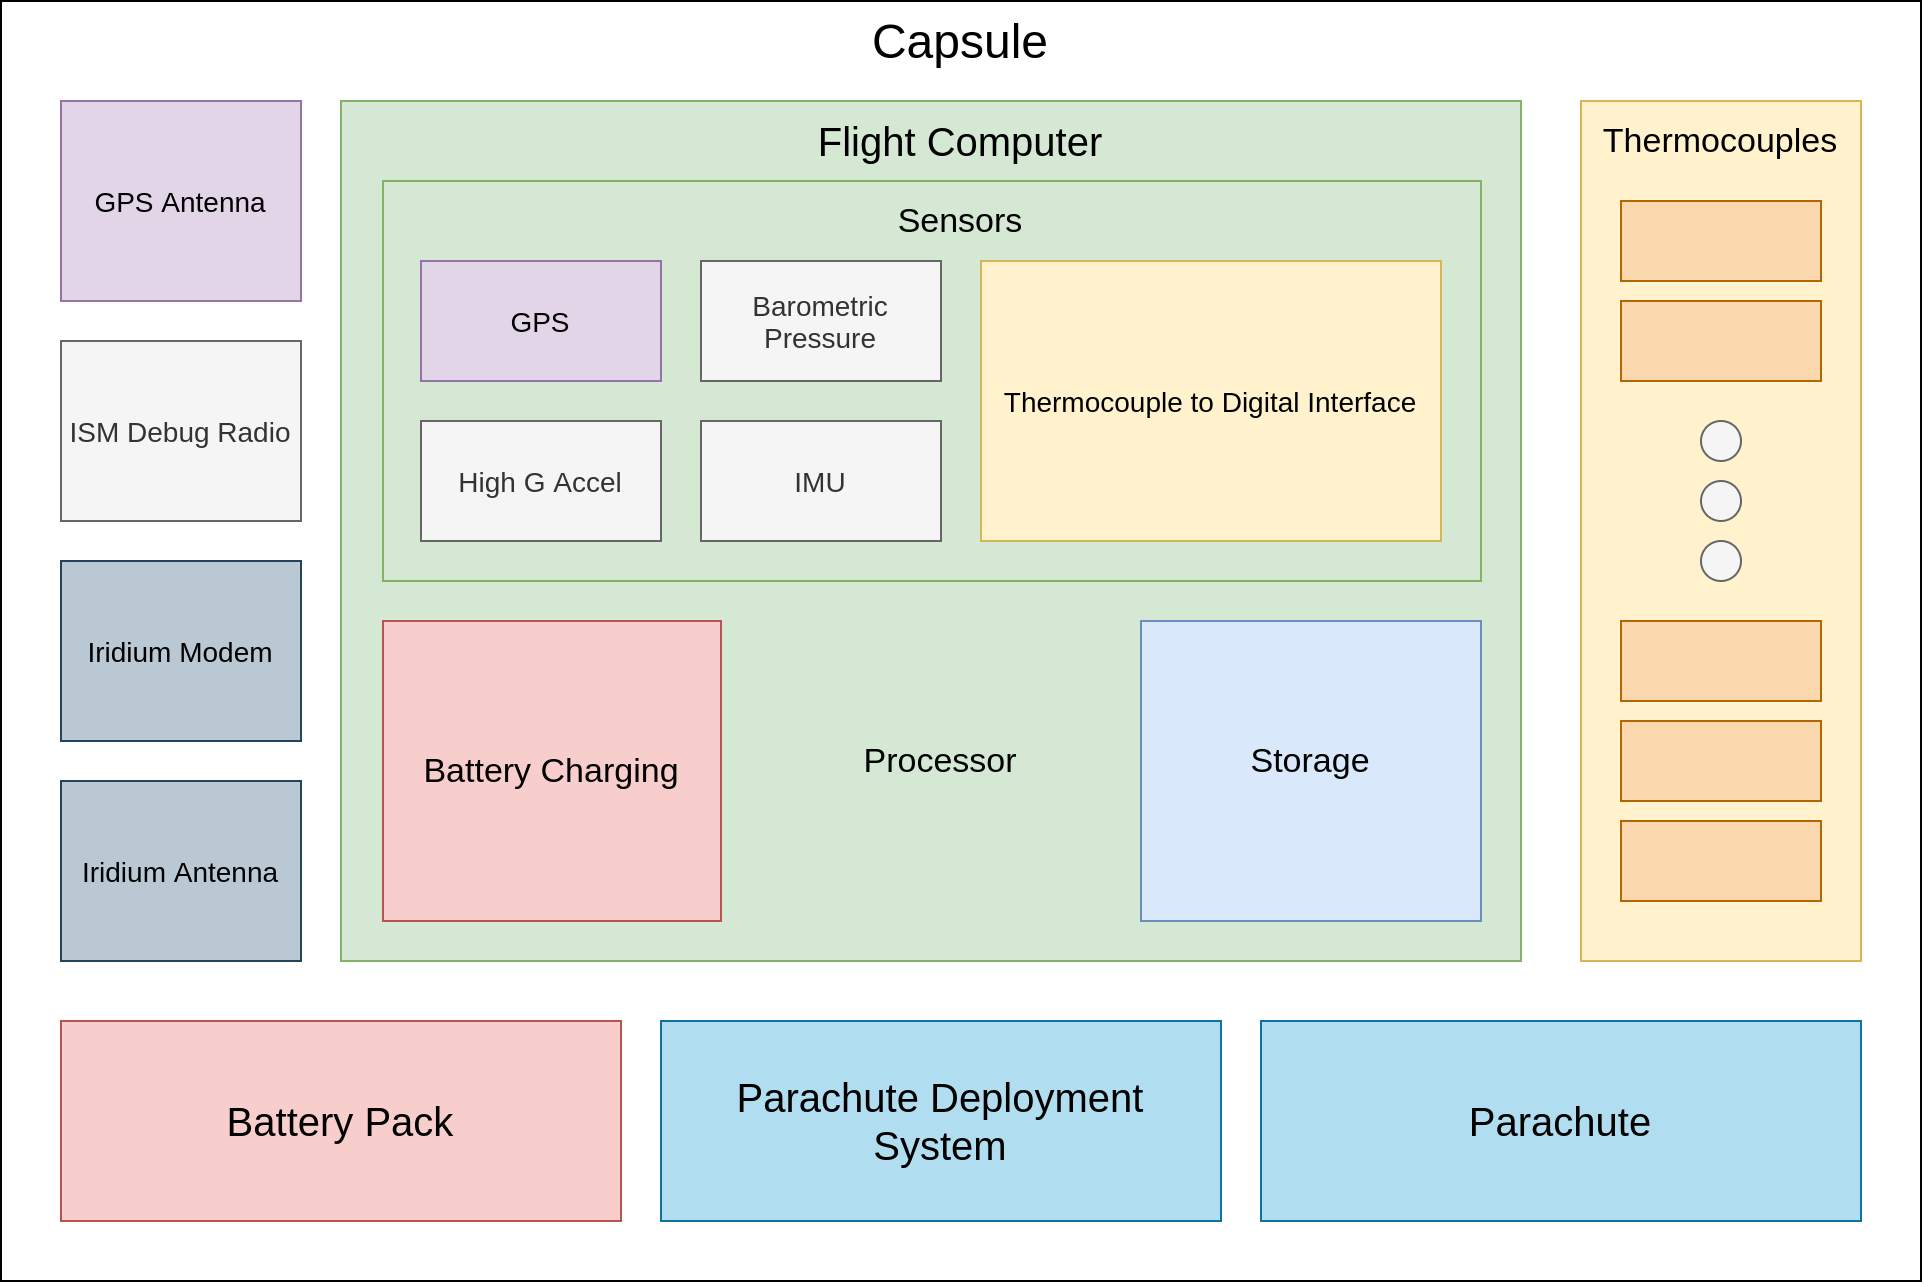
\includegraphics[width=\textwidth]{images/amtps-avionics.png}
	\caption{Capsule component overview, showing the various functional blocks.}
	\label{fig:capsule-overview}
\end{figure}


%%%%%%%%%%%%%%%%%%%%%%%%%%%%%%%%%%%%%%%%%%%%%%%%%%%%%%%%%%%%%%%%%%%%%%%%%%%%%
%%%%%%%%%%%%%%%%%%%%%%%%%%%%%%%%%%%%%%%%%%%%%%%%%%%%%%%%%%%%%%%%%%%%%%%%%%%%%
%%%%%%%%%%%%%%%%%%%%%%%%%%%%%%%%  APPENDIX
%%%%%%%%%%%%%%%%%%%%%%%%%%%%%%%%%%%%%%%%%%%%%%%%%%%%%%%%%%%%%%%%%%%%%%%%%%%%%
%%%%%%%%%%%%%%%%%%%%%%%%%%%%%%%%%%%%%%%%%%%%%%%%%%%%%%%%%%%%%%%%%%%%%%%%%%%%%
\section{Requirements}
\label{sec:requirements}
Based off of the most recent revision (\ddrev) of the flight test requirements document.

\begin{enumerate}
\item Instrumentation and telemetry
  \begin{enumerate}
	  \item Shall support betwen 8 and 20 thermocouples of varying type
	  \item Shall support up to 6 absolute pressure sensors
	  \item Shall support at least 1 intertial measurement unit (IMU)
	  \item Should support 1 heat flux sensor
	  \item Shall contain a GPS for recovery operations, accurate to with 100m
	  \item Capsule shall contain an internal barometric pressure sensor 
	  \item Telemetry data shall be collected at a minumum of 10Hz
	  \item Telemetry data shall be stored to onboard nonvolatile memory that will survive landing
	  \item Location telemetry shall be transmitted through a vehicle-to-ground system (e.g. Iridium satellite, Xbee)
	  \item Recovery location should be broadcasted at least once every 5 minutes post-flight
  \end{enumerate}
\item Activation and flight sequencing
  \begin{enumerate}
	  \item Shall be powered through the duration of the flight
	  \item Shall support continuous operation between -20 deg C and 80 deg C
	  \item Shall support pre-launch activation on the ground; should support low power mode prior to deployment
	  \item Shall detect and/or sense when deployment has occurred via interfacing with the launch vehicle
	  \item Shall transmit in-flight telemetry with position information
	  \item In-flight telemetry should contain capsule velocity 
	  \item Shall trigger parachute deployment at a specified time
  \end{enumerate}
\item Physical properties
\item Avionics hardware shall weigh under or around 0.5kg
\item Shall cost under \$3,000
\end{enumerate}




%%%%%%%%%%%%%%%%%%%%%%%%%%%%%%%%%%%%%%%%%%%%%%%%%%%%%%%%%%%%%%%%%%%%%%%%%%%%%
%%%%%%%%%%%%%%%%%%%%%%%%%%%%%%%%%%%%%%%%%%%%%%%%%%%%%%%%%%%%%%%%%%%%%%%%%%%%%
%%%%%%%%%%%%%%%%%%%%%%%%%%%%%%%%  DESIGN
%%%%%%%%%%%%%%%%%%%%%%%%%%%%%%%%%%%%%%%%%%%%%%%%%%%%%%%%%%%%%%%%%%%%%%%%%%%%%
%%%%%%%%%%%%%%%%%%%%%%%%%%%%%%%%%%%%%%%%%%%%%%%%%%%%%%%%%%%%%%%%%%%%%%%%%%%%%
\section{Subsystem Design}
\label{sec:ss-design}

\subsection{Main command and data handling}

Using off the shelf processors for convenience, and also to avoid bottlenecks in prototyping due to unpredictable chip shortages. Currently, two development boards from Adafruit are being used to prototyping and are listed below in Table \ref{tab:processors}\footnote{TPM: Temperature and Pressure Measurement}\footnote{CDH: Command and Data Handling}. The diagram in Figure \ref{fig:main-overview} provides a general overview of the organization of electronic hardware within the capsule. 

\begin{figure}[h!]
	\centering
	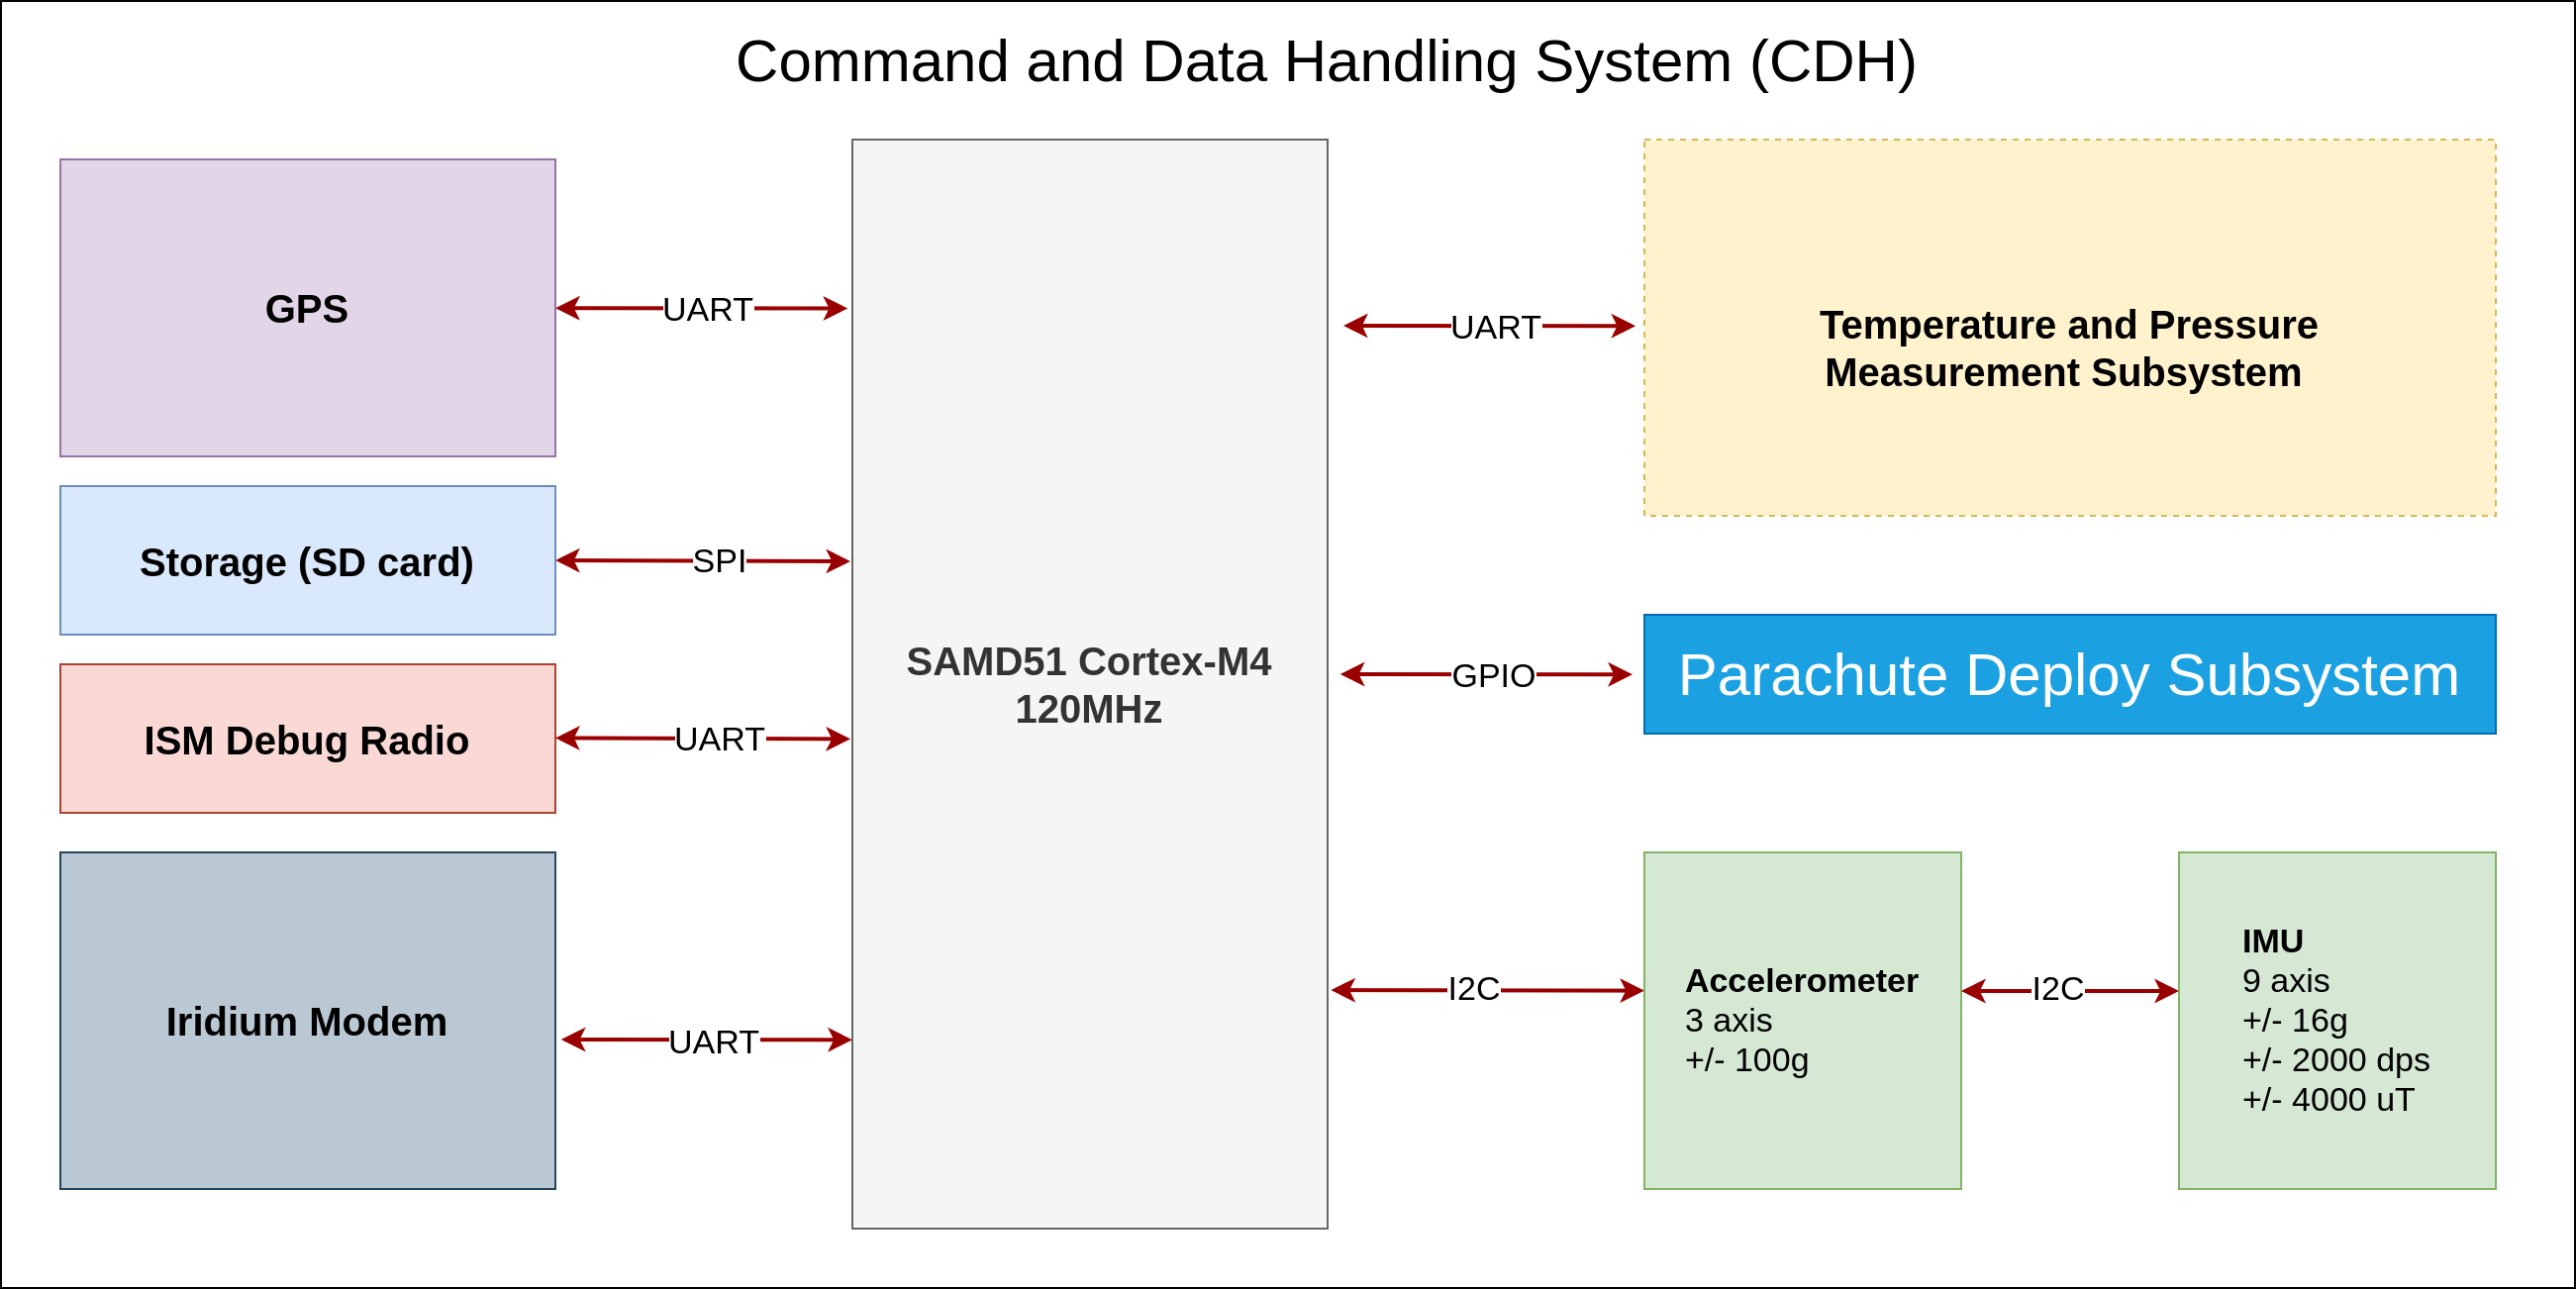
\includegraphics[width=\textwidth]{images/amtps-main-system.png}
	\caption{Main functional components of the capsule and the communication buses between them.}
	\label{fig:main-overview}
\end{figure}


\begin{table}[h!]	
	\caption{List of processors used and their capabilities.}
	\begin{tabular}{l | c c m{5cm}}
		Part & Description & Role & Product Link \\
		\hline
		(2) Feather M0 Basic Proto & Cortex-M0 @ 48 MHz & TPM and IMU processor & \url{https://www.adafruit.com/product/2772}\\
		Feather M4 Express & Cortex-M4 @ 120Mhz & CDH Processor & \url{https://www.adafruit.com/product/3857} 
	\end{tabular}
	\label{tab:processors}
\end{table}

Shown in Fig. \ref{fig:cdh-prototype} is the assembled prototype of the main board.
\begin{figure}[h!]
	\centering
	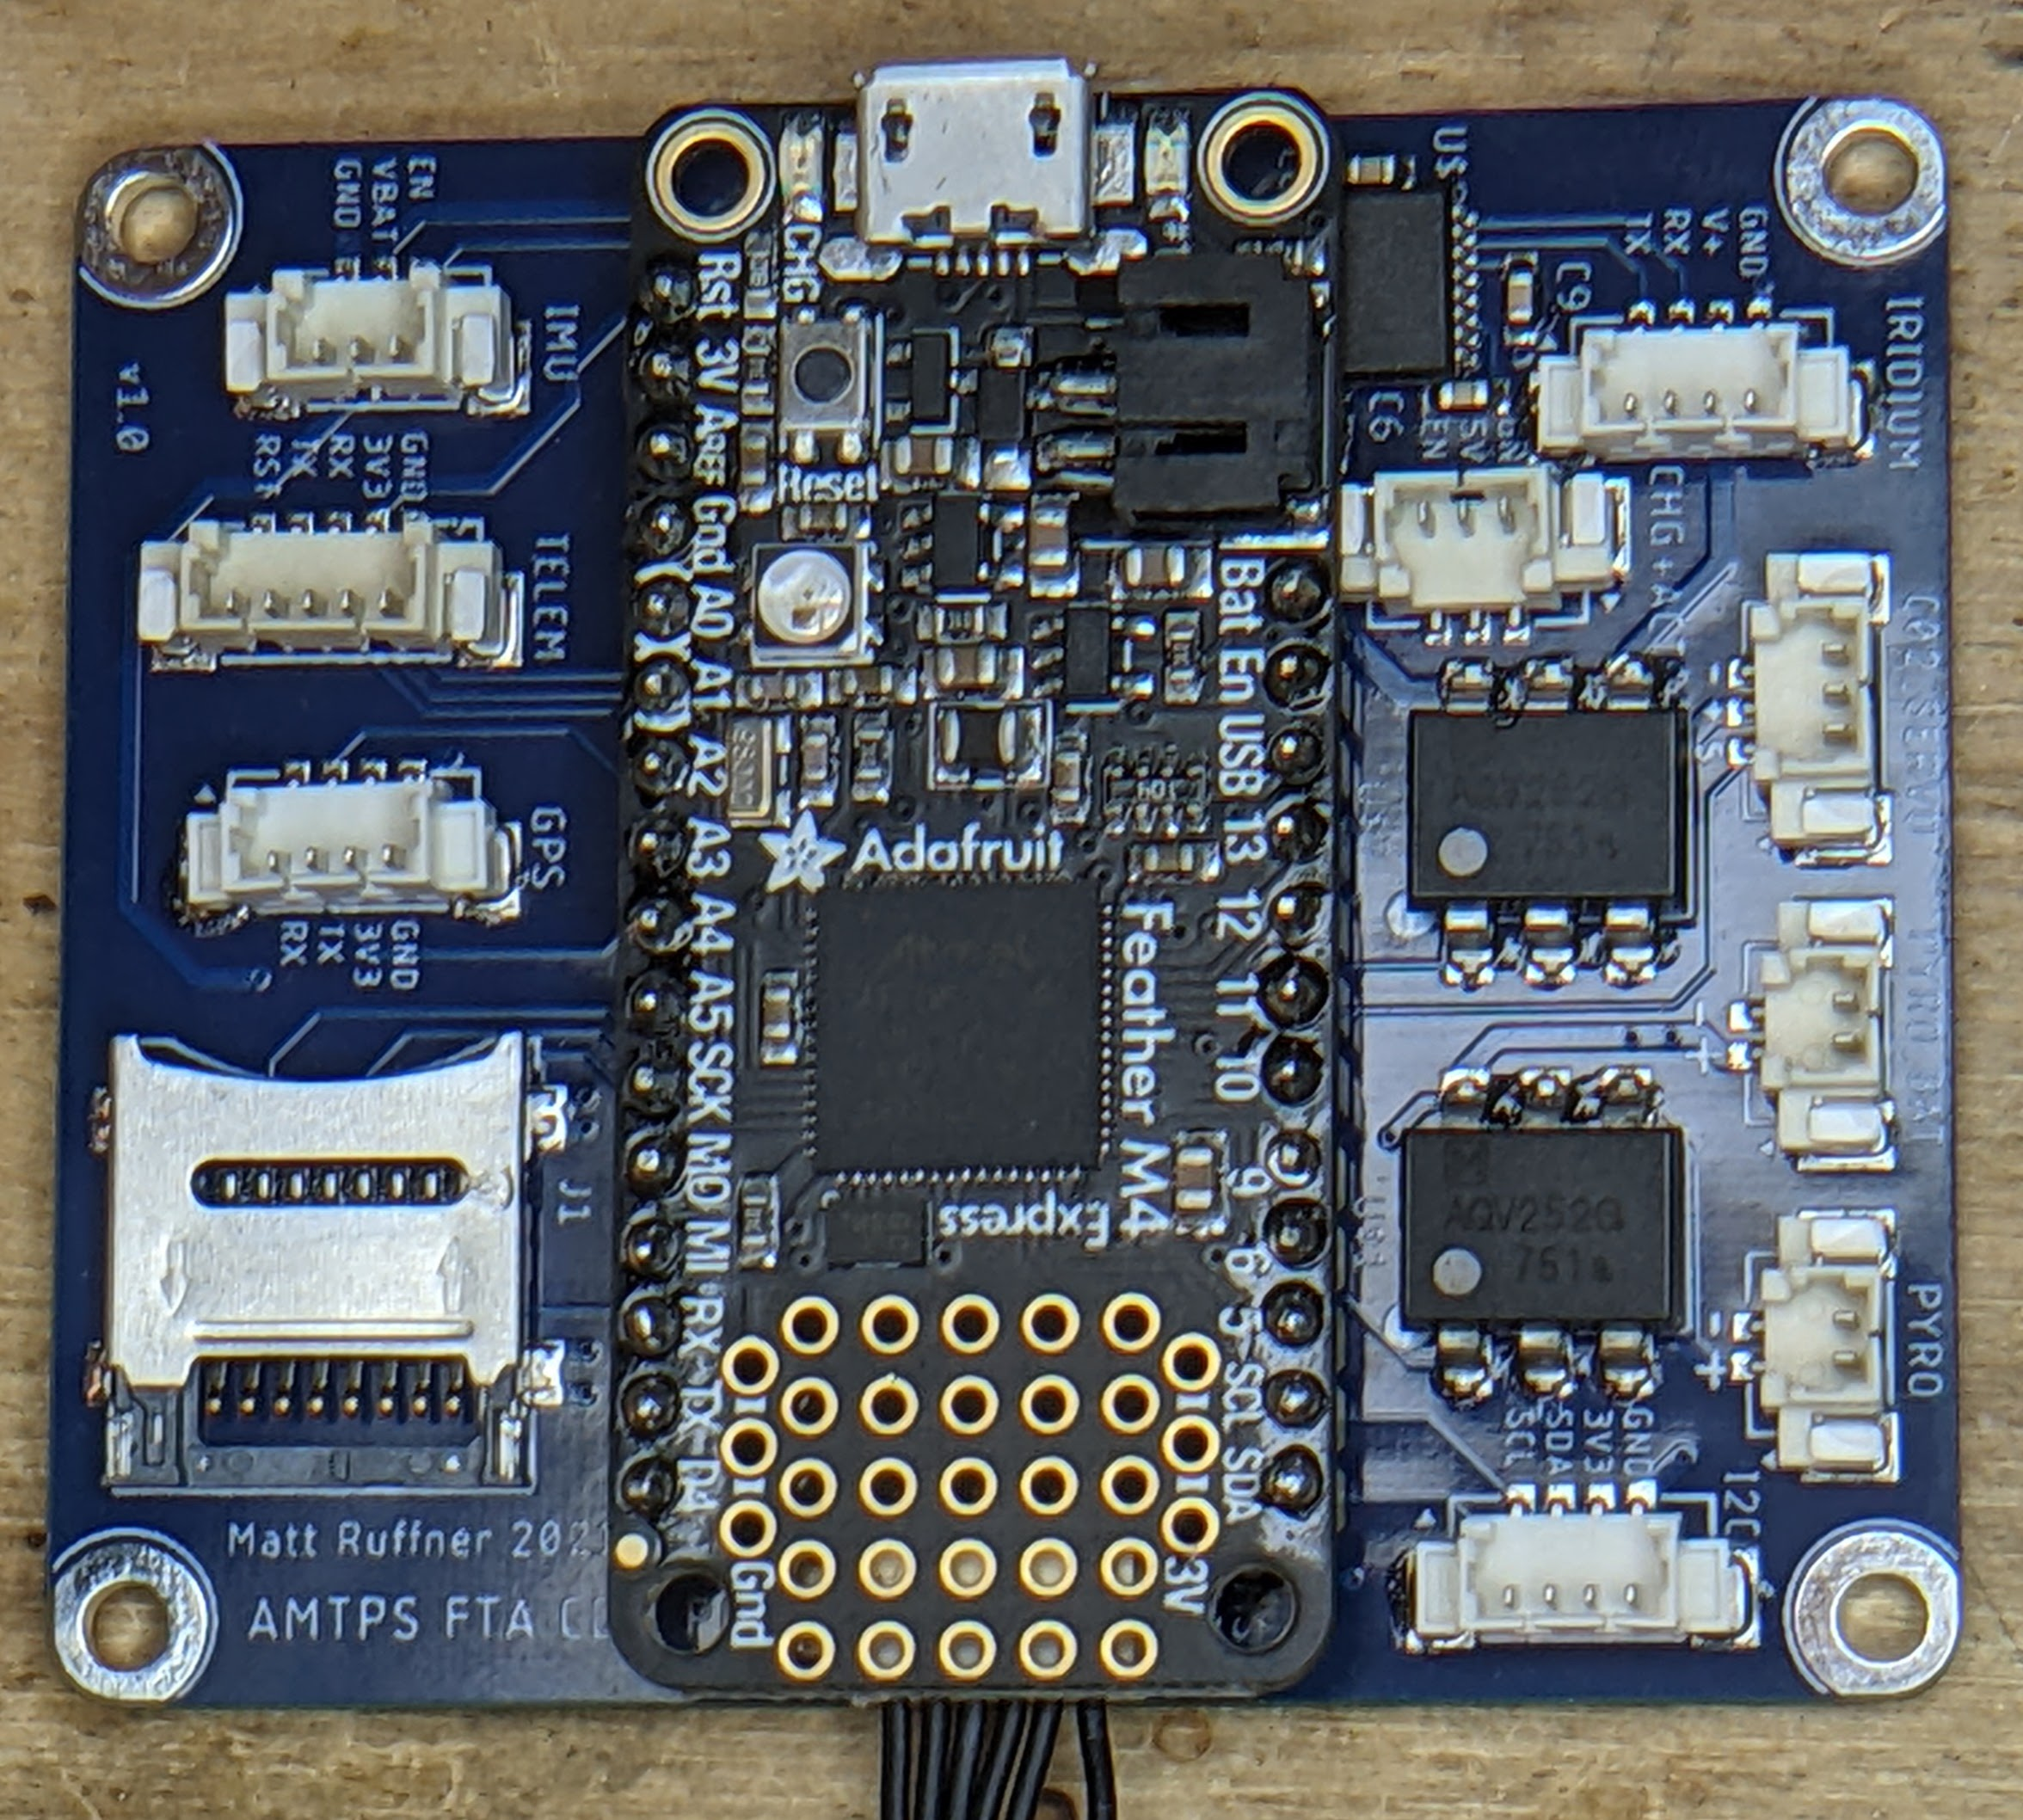
\includegraphics[width=10cm]{images/main-board}
	\caption{Assembled CDH main board.}
	\label{fig:cdh-prototype}
\end{figure}


%%%%%%%%%%%%%%%%%%%%%%%%%%%%%%%%%%%%%%%%%%%%%%%%%%%%%%%%%%%%%%%%%%%%%%%%%%%%%
%%%%%%%%%%%%%%%%%%%%%%%%%%%%%%%%%%%%%%%%%%%%%%%%%%%%%%%%%%%%%%%%%%%%%%%%%%%%%
\subsection{Temperature and Pressure Measurement}
The temperature and pressure measurement (TPM) Subsystem (TPMS) supports collection of several datapoints needed for recreating the heating environment of reentry. The diagram in Figure \ref{fig:tpms-overview} shows an overview of the temperature and pressure monitoring subsystem. Images of the TC to digital breakout and TPMS interface boards are shown in Figs. \ref{fig:tpms-proto} and \ref{fig:tc-board-bottom}.

In order to support the large number of TCs required in the capsule, a breakout board supporting 6 of the MCP9600T-E/MX series TC to digital converter was designed. This TC converter chip was selected due to its support for a wide variety of TC types (K, J, T, N, S, E, B and R)\footnote{\url{https://www.digikey.com/en/products/detail/microchip-technology/MCP96L00T-E-MX/9606988}}, as well as its chainable I$^2$C interface, allowing more sensing elements to connected with less wiring (similar SPI based conversion chips have a chip select line per chip that would restrict the number of pins available for other capsule functionality).


For pressure meausrement, Honeywell sensing solutions temperature compensated absolute digital pressure sensors were selected and are shown in Table \ref{tab:pressure-sensors}. These single port absolute pressure sensors are available with a variety of sensitivities, allowing a different sensor to be exchanged later on in the design process if it is determined that the current predicted pressure environment is no longer accurate.


\begin{table}[h!]
	\caption{List of pressure sensors and their capabilities}
	\begin{tabular}{c | c m{9cm}}
		Part & Measurement Range & Product Link \\
		\hline
		SSCSRNN015PA3A3 & 0-103.42 kPa & \url{https://www.digikey.com/en/products/detail/honeywell-sensing-and-productivity-solutions/SSCSRNN015PA3A3/2416212}\\
		SSCSRNN1-6BA7A3 & 0-160 kPa & \url{https://www.digikey.com/en/products/detail/honeywell-sensing-and-productivity-solutions/SSCSRNN1-6BA7A3/2416214} 
	\end{tabular}
\label{tab:pressure-sensors}
\end{table}

\begin{figure}[H]
	\centering
	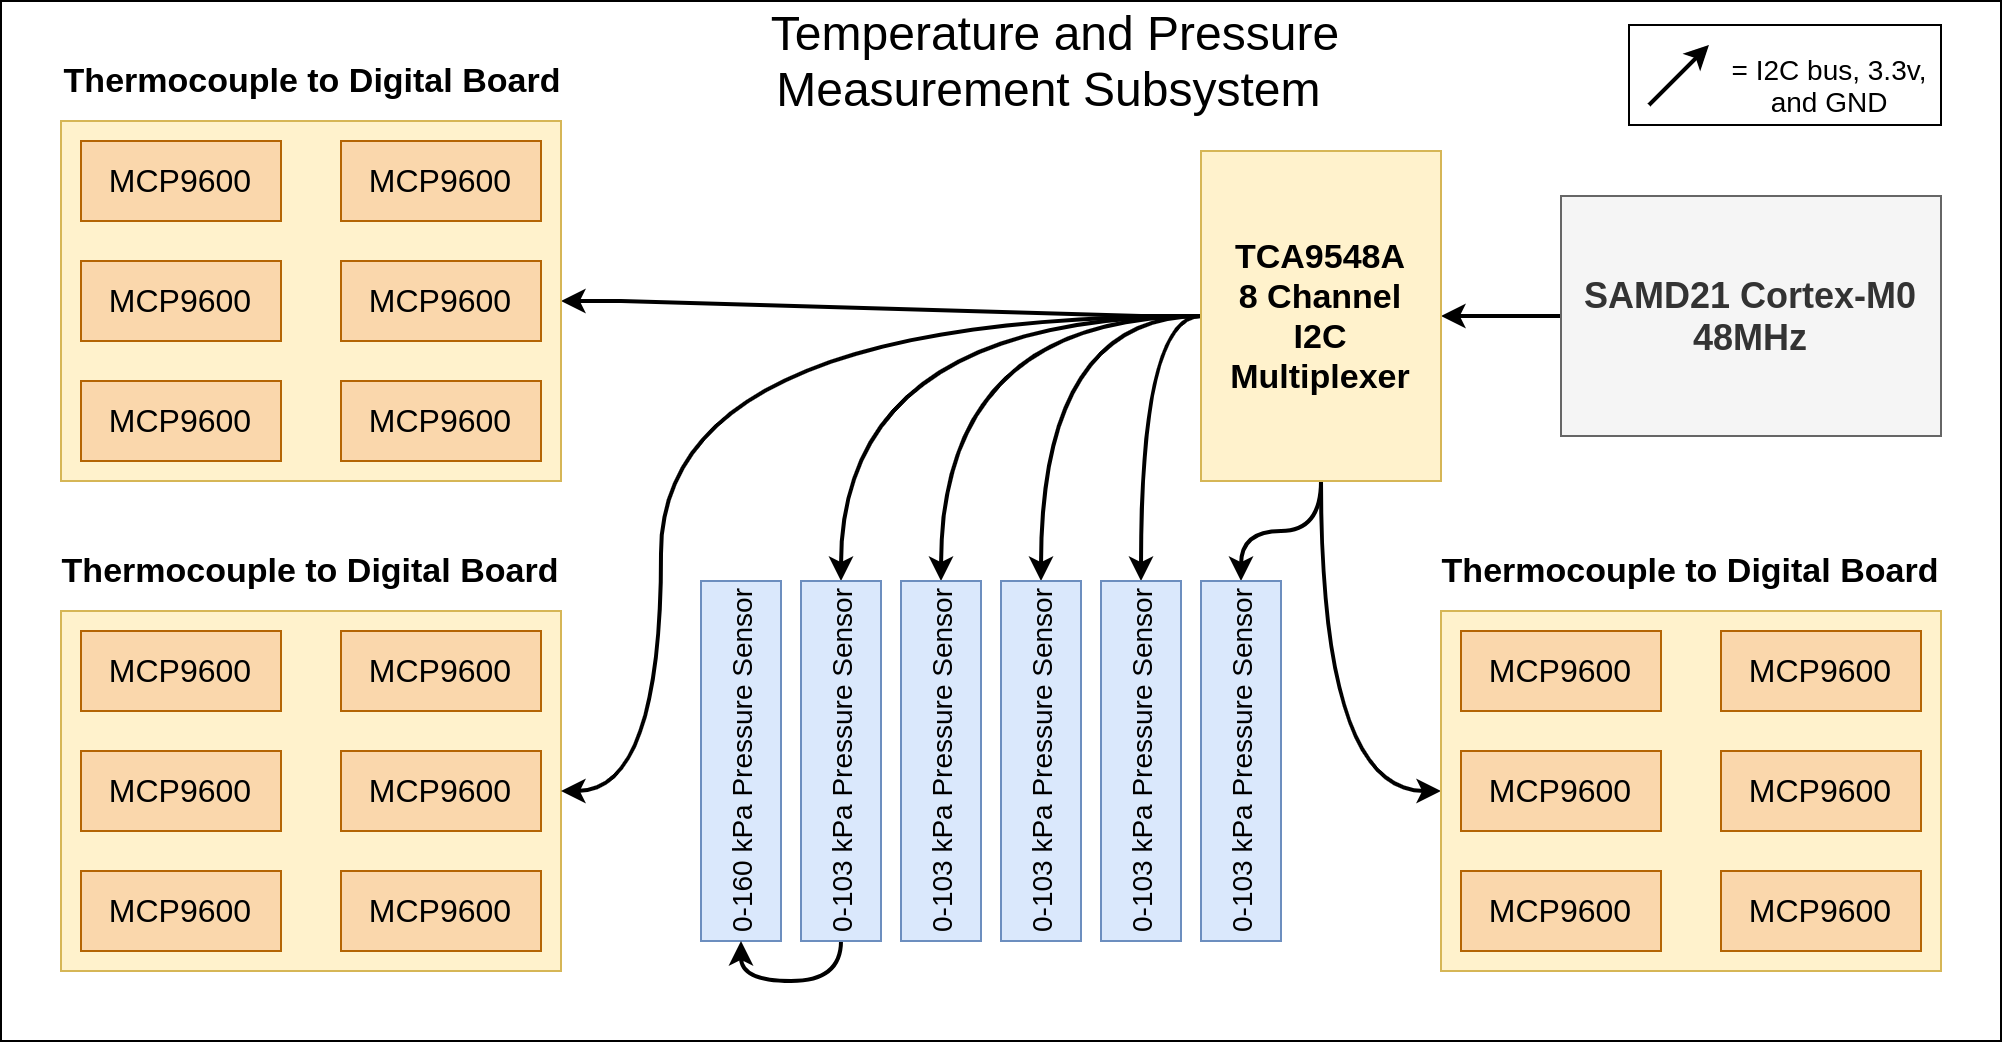
\includegraphics[width=\textwidth]{images/amtps-temp-pressure-subsystem.png}
	\caption{Functional decomposition of the TPMS.}
	\label{fig:tpms-overview}
\end{figure}

Shown in Fig. \ref{fig:tpms-proto} is the assembled prototype of the TPMS breakout board that interfaces to the CDH board and the TC breakouts.
\begin{figure}[H]
	\centering
	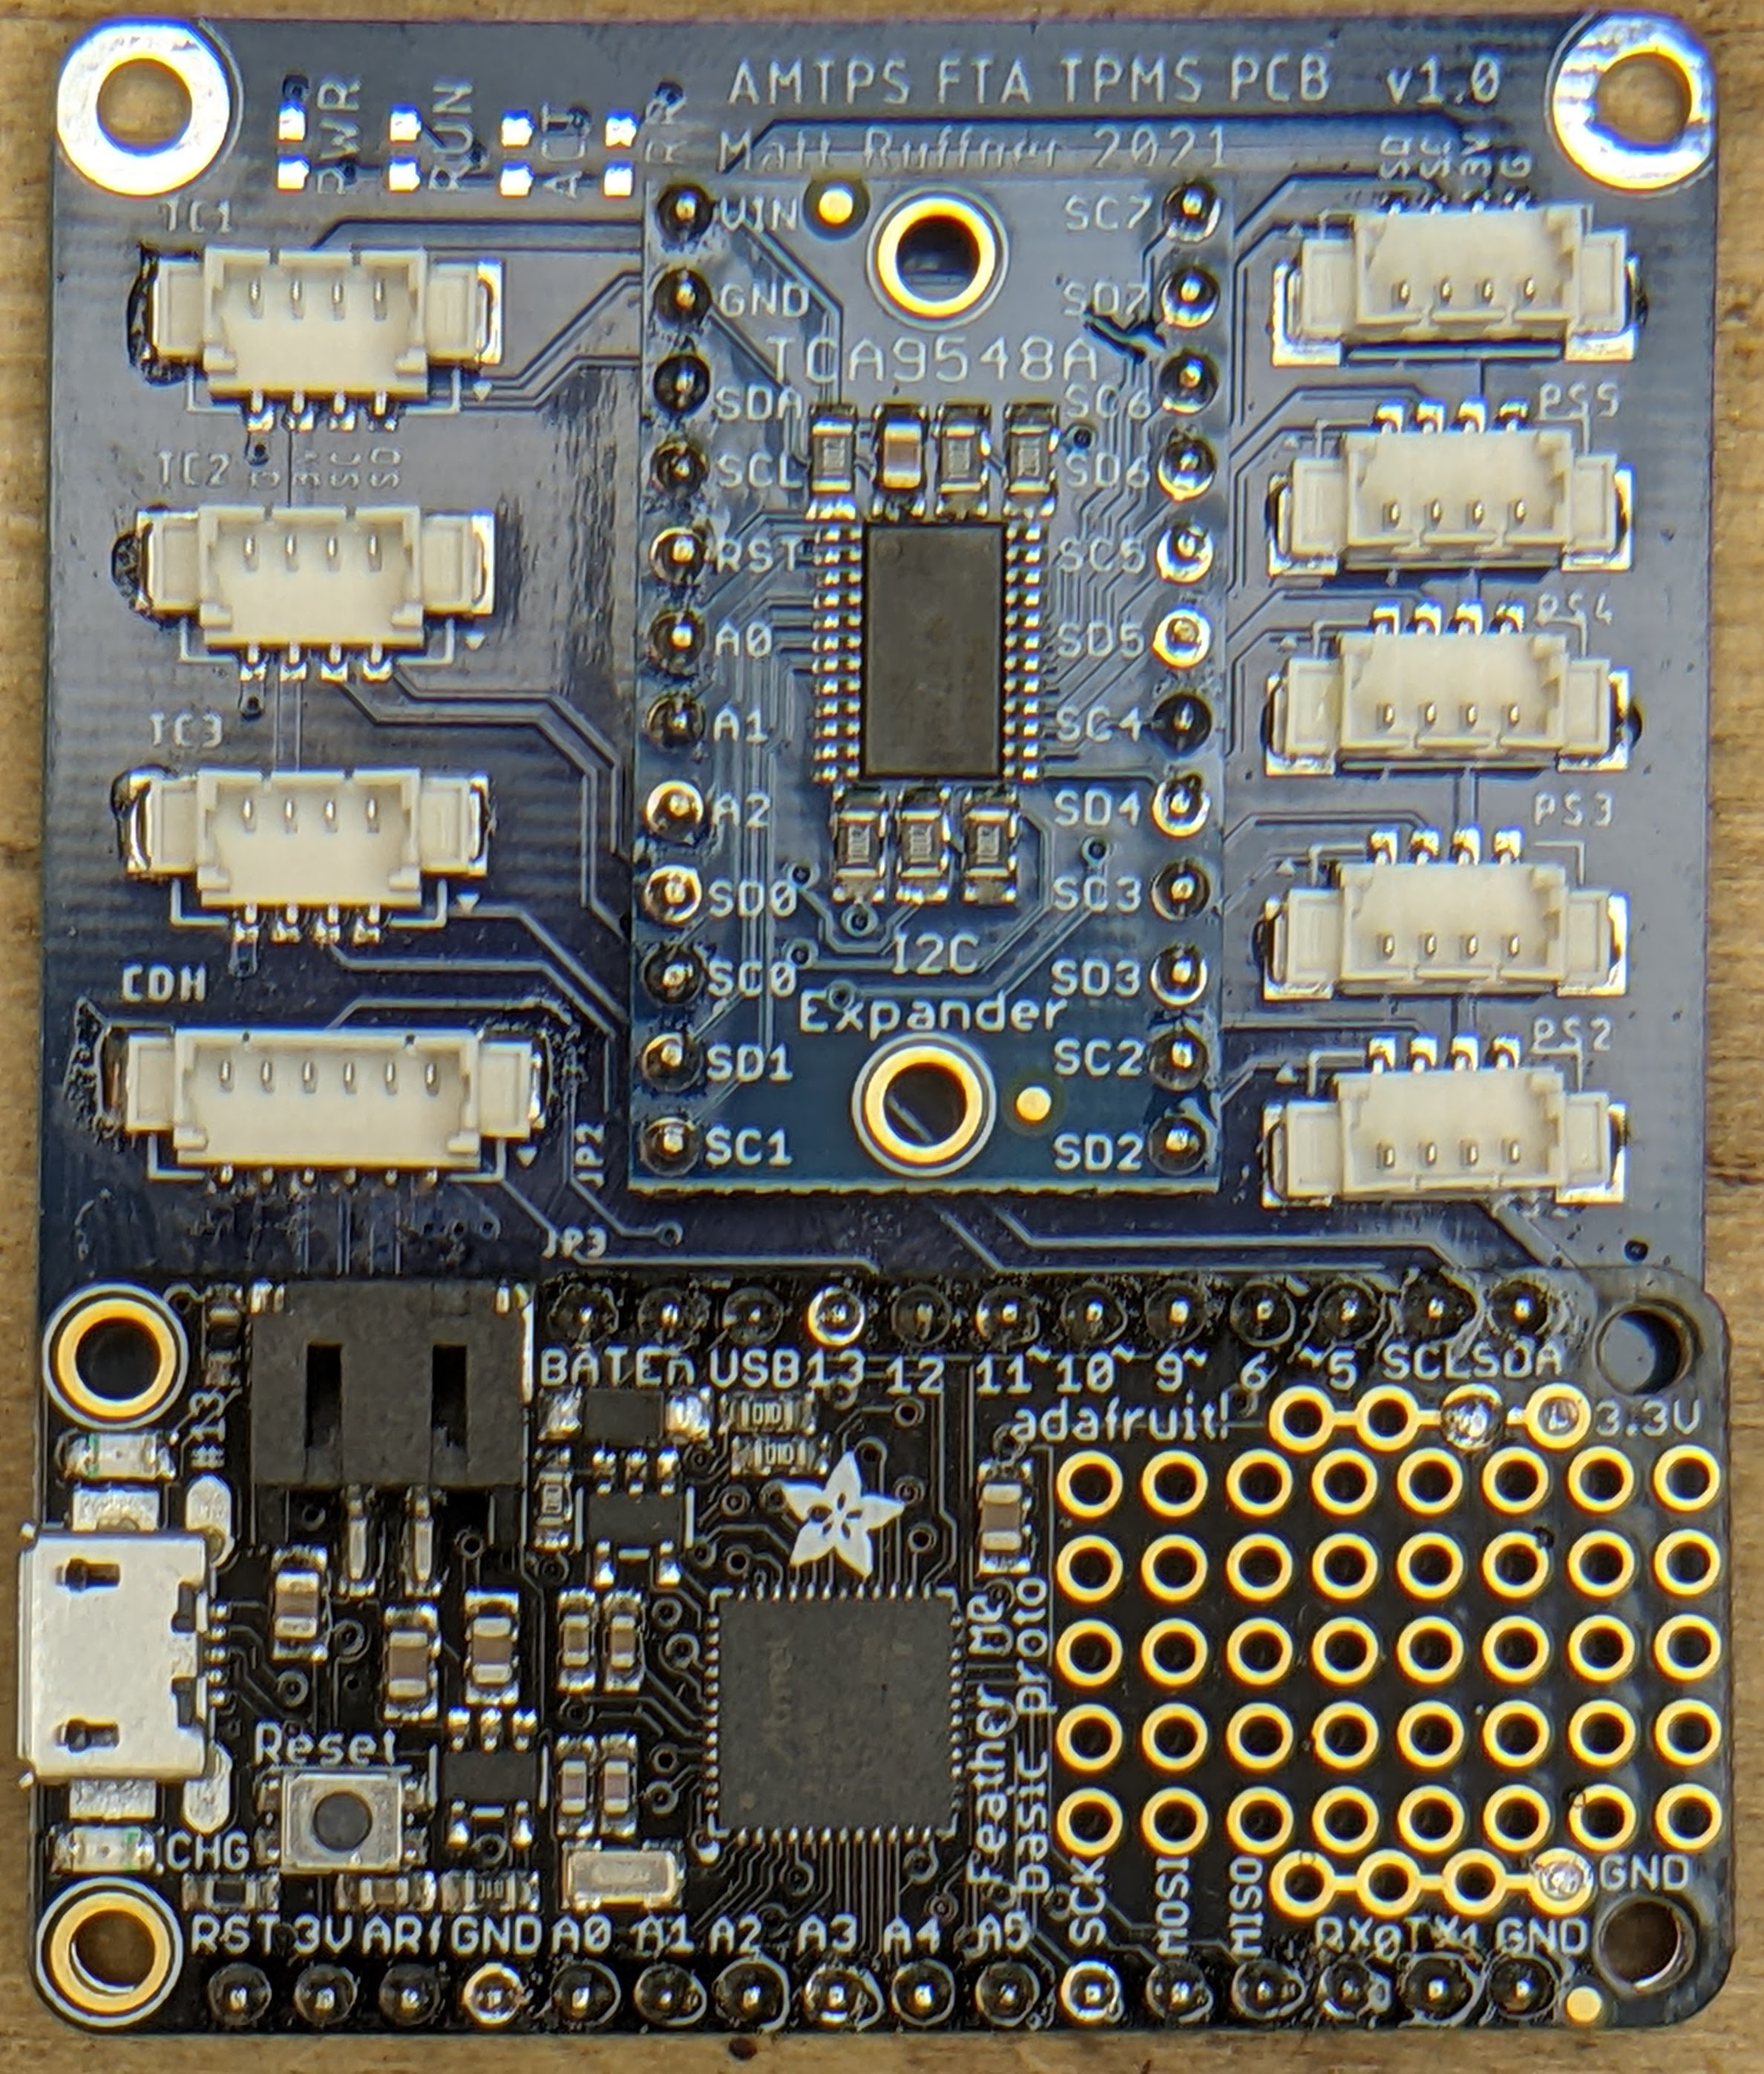
\includegraphics[width=10cm]{images/tpms-breakout}
	\caption{Assembled TPMS breakout board.}
	\label{fig:tpms-proto}
\end{figure}

Shown in Fig. \ref{fig:tc-board-bottom} is the TC to digital breakout board, two of which will be used for a total of 12 TC channels.
\begin{figure}[H]
	\centering
	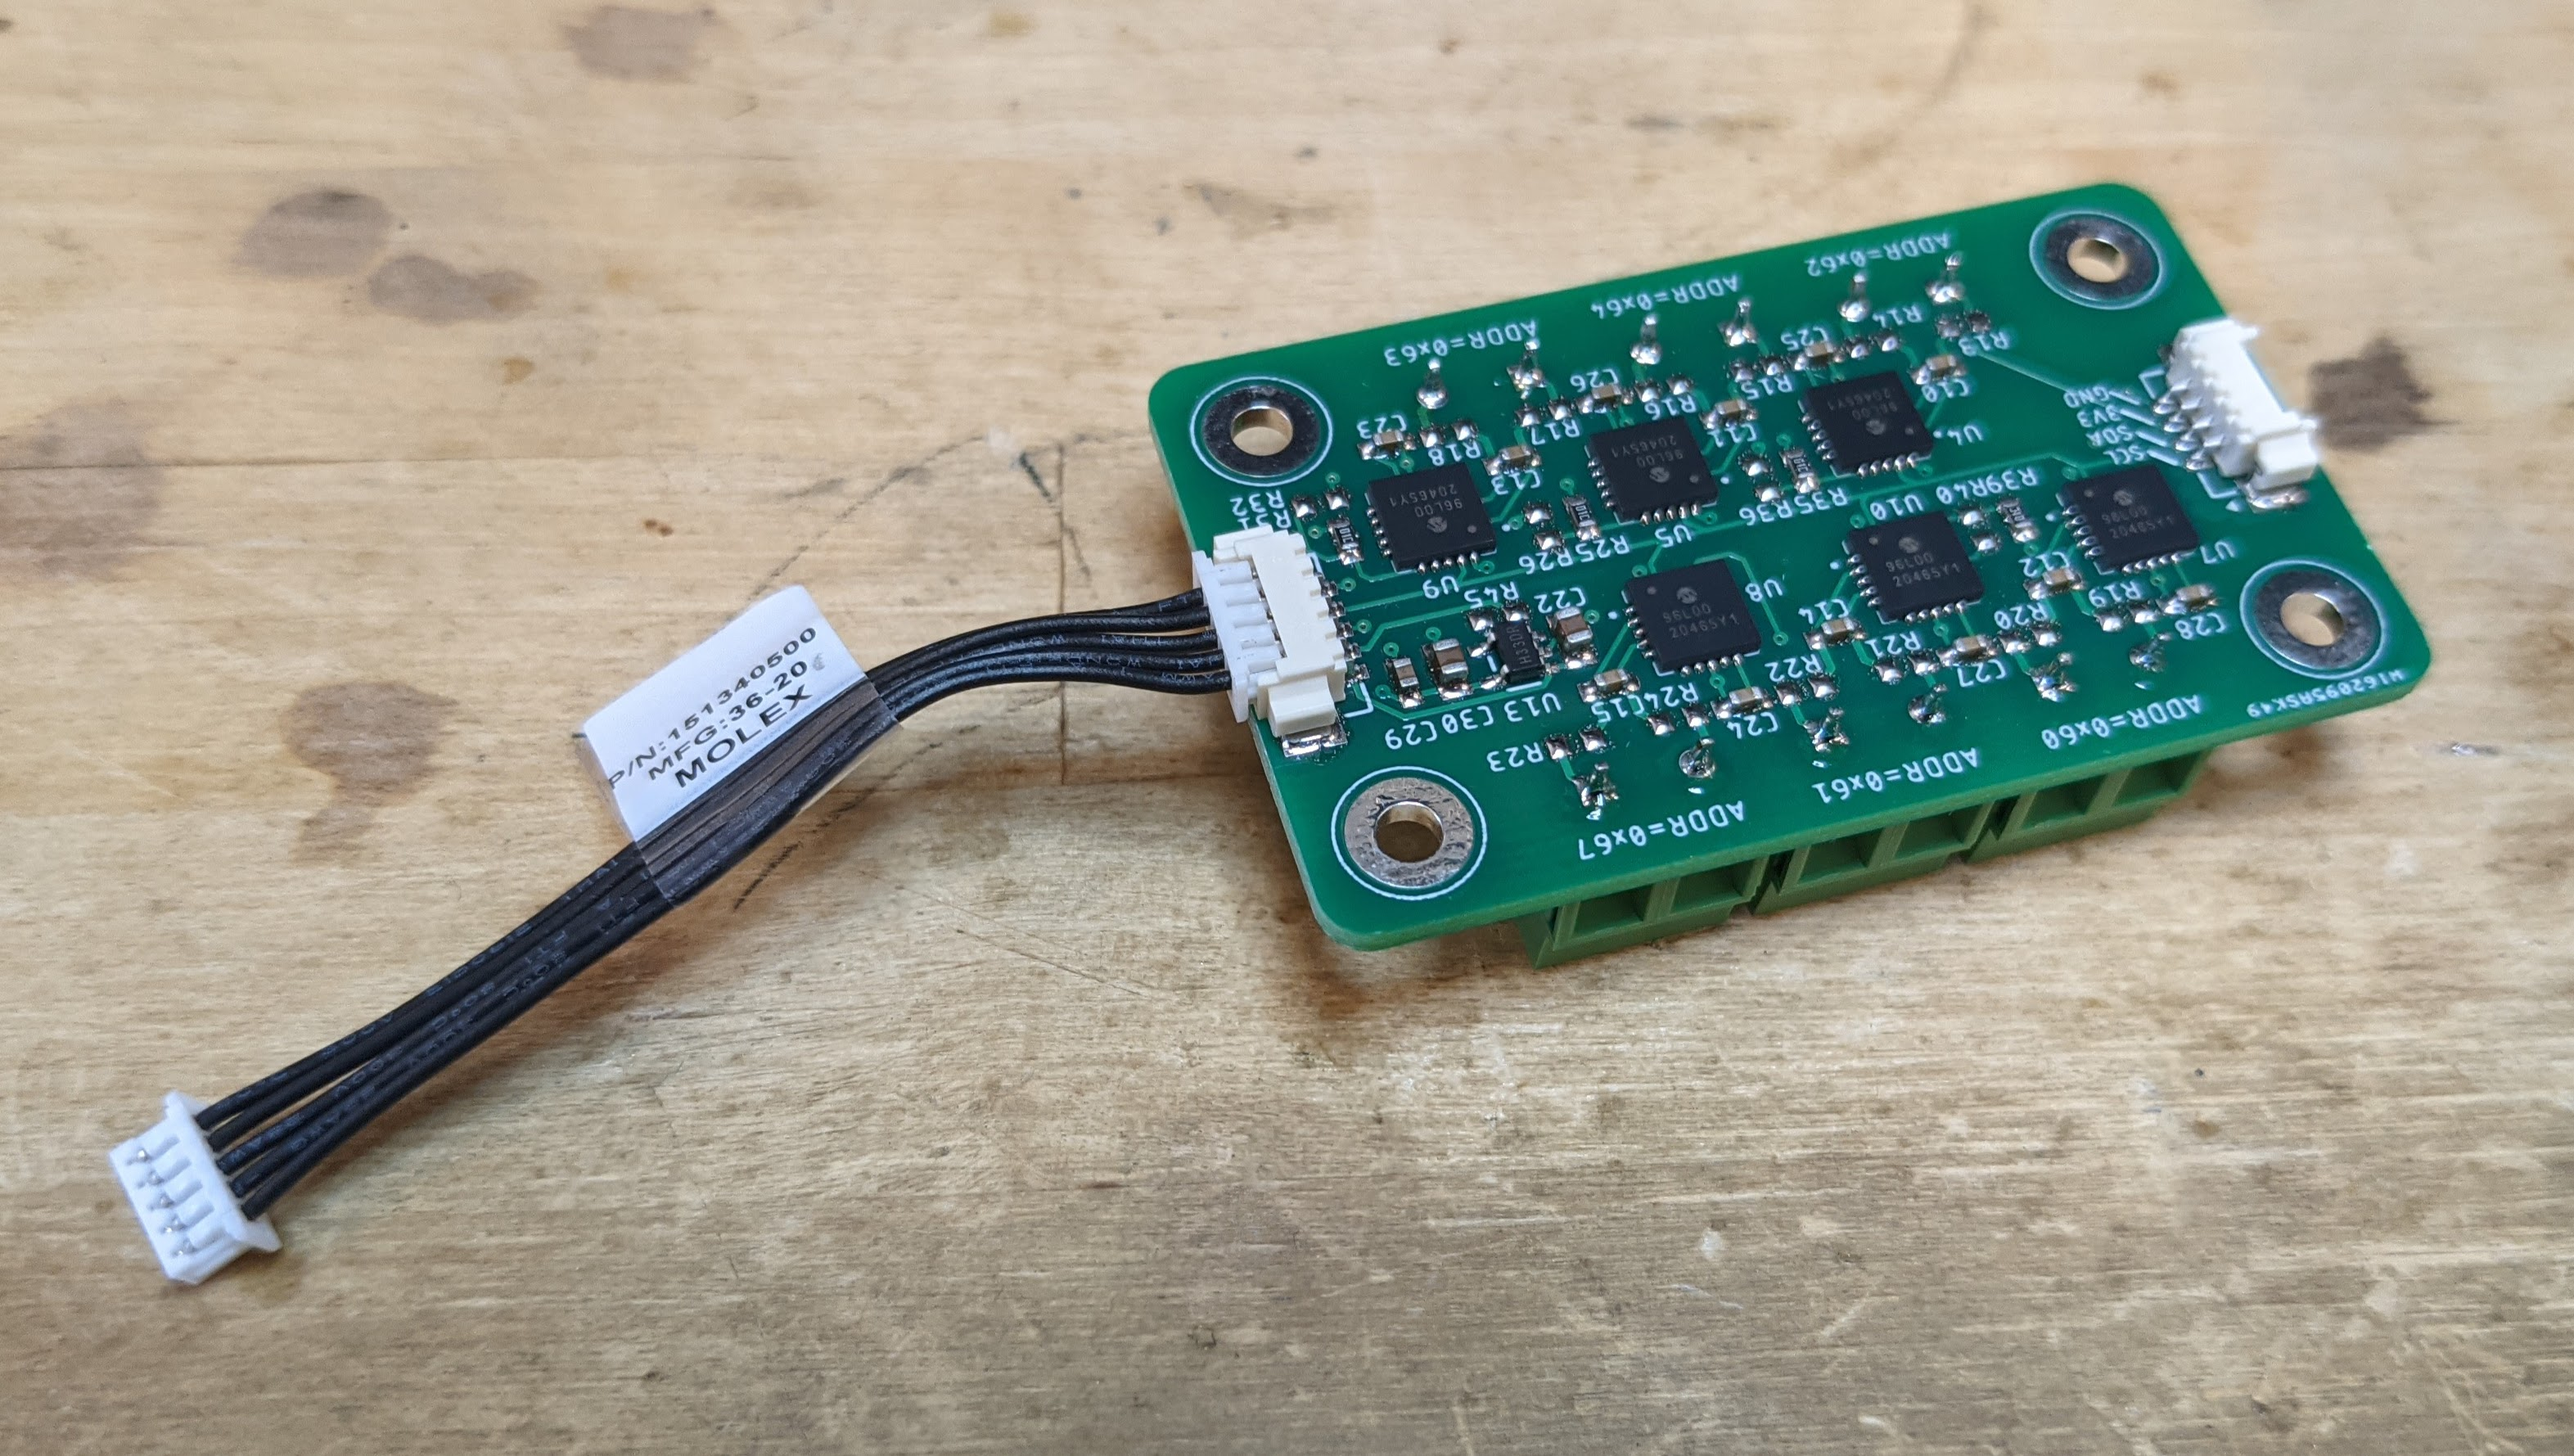
\includegraphics[width=13cm]{images/tc-board-bottom}
	\caption{Bottom of V1 Evaluation board for MCP9600 TC to digital converter}
	\label{fig:tc-board-bottom}
\end{figure}


\subsection{Inertial Measurement}
A breakout board for the H3LIS100DL~\footnote{\url{https://www.digikey.com/en/products/detail/stmicroelectronics/H3LIS100DL/7313278}} +/- 100g accelerometer has been designed to help in the evaluation of this IC as an effective way to measure acceleration loads on the capsule. In addition to a +/- 100g 3-axis accelerometer, a lower dynamic range 9 axis acceleromter+gyroscope chip will also be included (ICM-20949).

\begin{figure}[H]
	\centering
	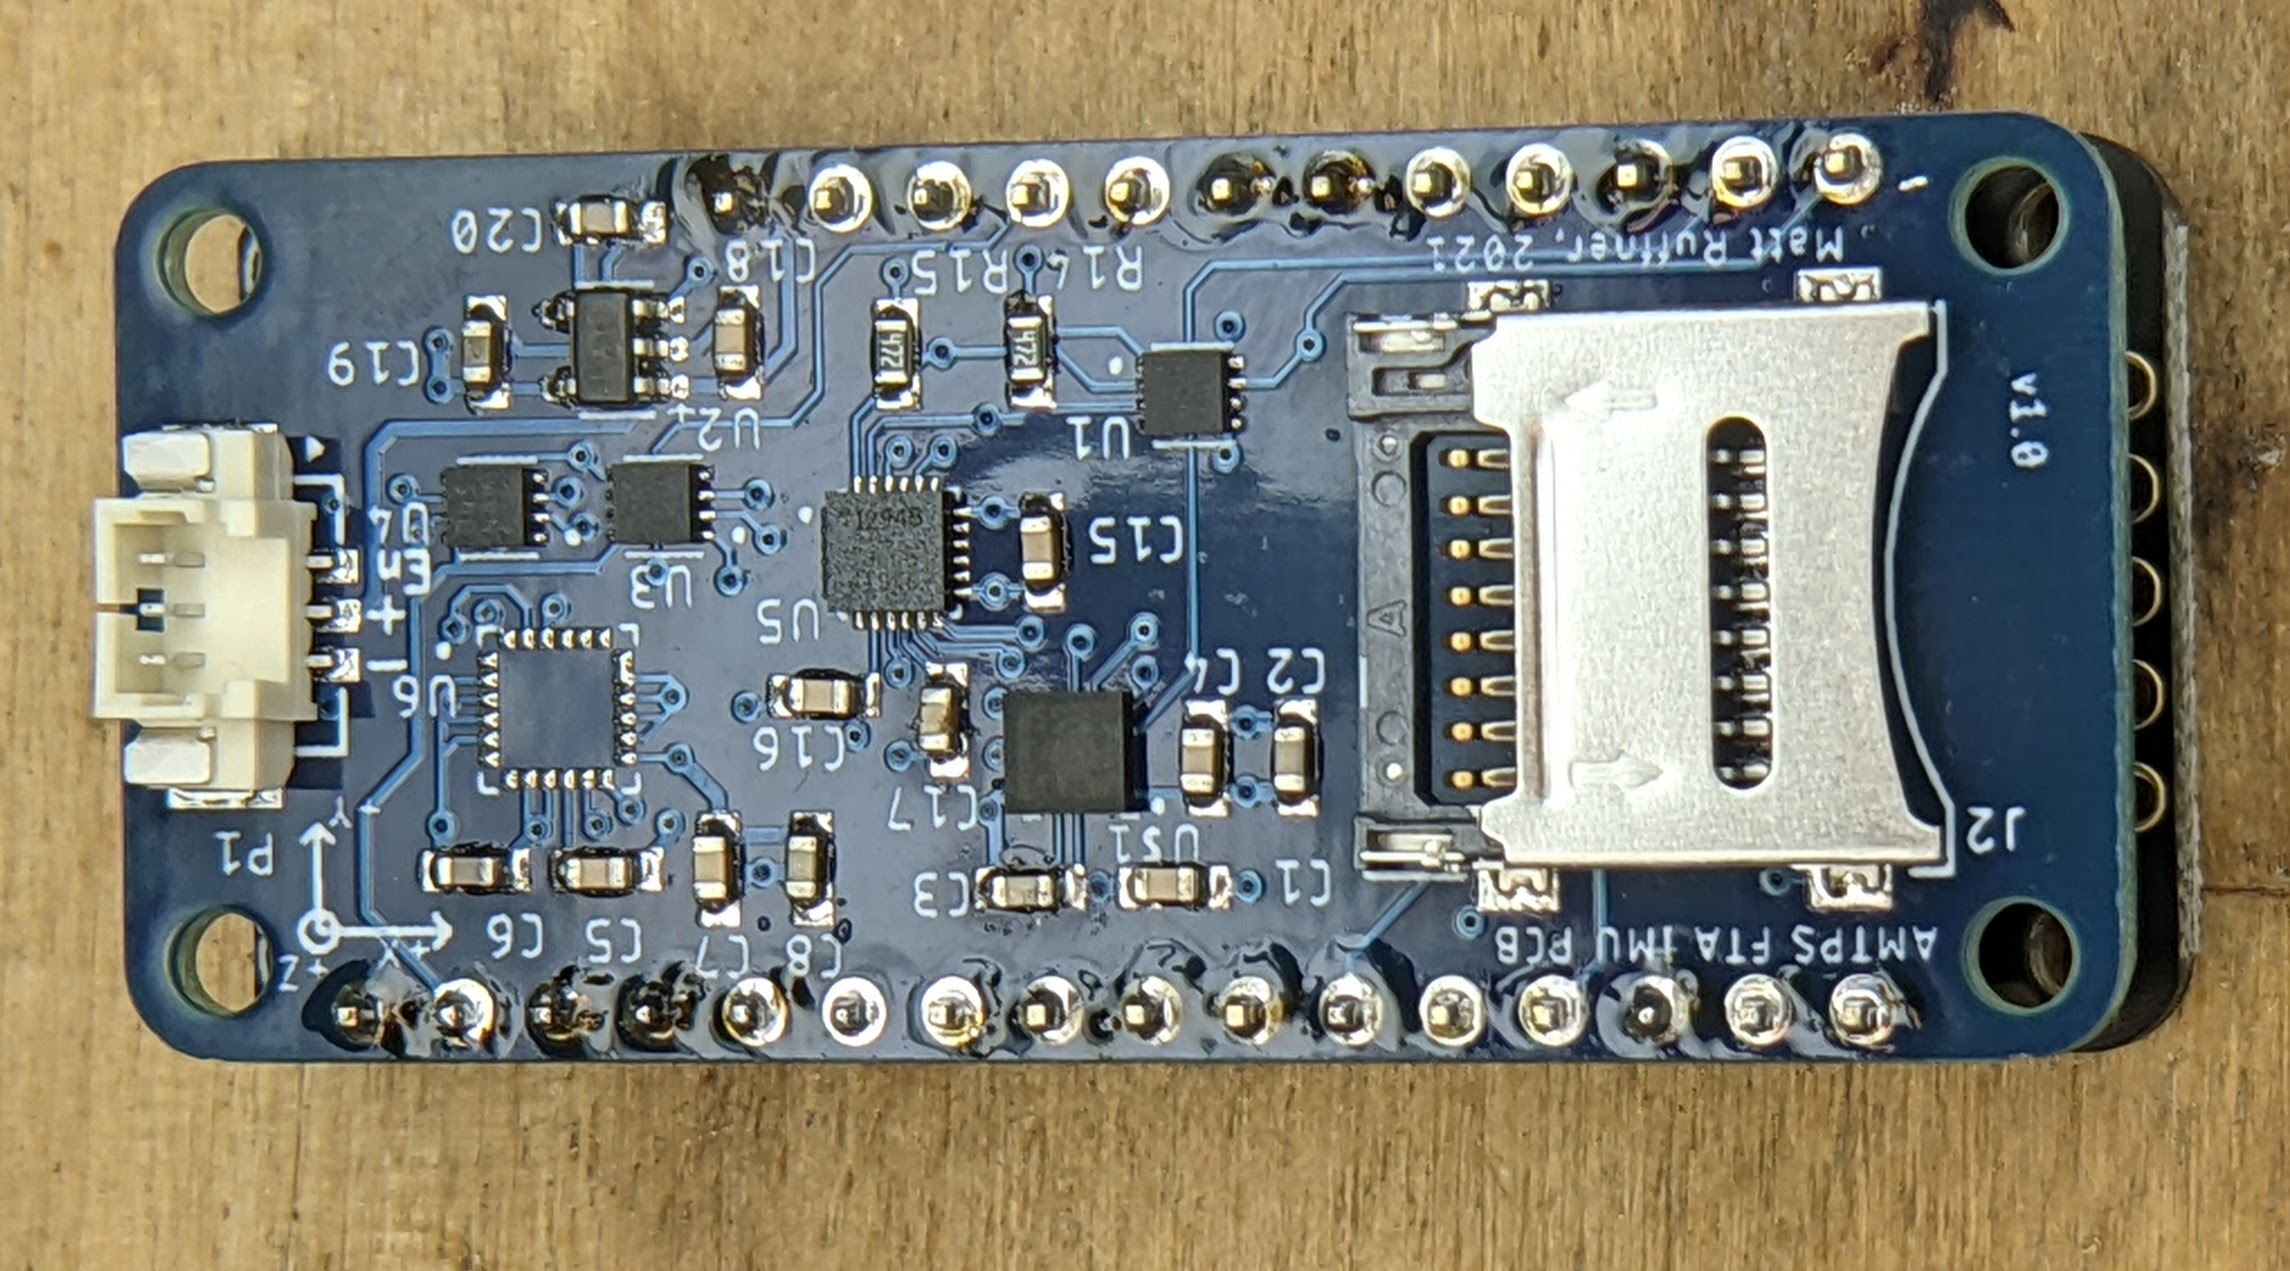
\includegraphics[width=10cm]{images/imu-breakout}
	\caption{Assembled IMU logger with ICM-20948 9-axis IMU and H3LIS100 3-axis 100g accelerometer.}
	\label{fig:imu-breakout}
\end{figure}

%%%%%%%%%%%%%%%%%%%%%%%%%%%%%%%%%%%%%%%%%%%%%%%%%%%%%%%%%%%%%%%%%%%%%%%%%%%%%
%%%%%%%%%%%%%%%%%%%%%%%%%%%%%%%%%%%%%%%%%%%%%%%%%%%%%%%%%%%%%%%%%%%%%%%%%%%%%
\subsection{Telemetry}

Iridium modem to send GPS coordinates for recovery operations. University of Kentucky has purchased an Iridium modem for use in this project and has an account providing message credits. Additional vehicle-to-ground telemetry would be reassuring as the Iridium network can be unreliable for short periods of time. It is unclear whether this would be achievable with a COTS radio link (such as XBee or LORA) that would not require FCC certification. This requires coordination with launch site for tracking with a directional antenna and other hardware setup. The appeal of the Iridium is we get an email with the GPS coordinates of the capsule and we can tell the recovery crew the location of the capsule from anywhere. 


%%%%%%%%%%%%%%%%%%%%%%%%%%%%%%%%%%%%%%%%%%%%%%%%%%%%%%%%%%%%%%%%%%%%%%%%%%%%%
%%%%%%%%%%%%%%%%%%%%%%%%%%%%%%%%%%%%%%%%%%%%%%%%%%%%%%%%%%%%%%%%%%%%%%%%%%%%%
\subsection{Parachute Deployment}
There will be a main and drogue chute. Initial drogue chute deployment will be propelled by a CO$_2$ cartridge puncture system which has a servo actuated trigger. Servo control signal pins are allotted on the main CDH processor and configured in software to trigger when necessary. Release of the drogue chute will be facilitated by pyrotechnic cutters which will be triggered sometime after drogue chute deployment.

The software to trigger the drogue based on barometric pressure is functional. There is a necessary calibration step where, once at white sands, the pressure at ground level would be programmed into the capsule via the wireless debug interface.

Current plans to decide correct deployment time are to use capsule internal barometric pressure, possibly in combination with one of the external pressure sensors.


%%%%%%%%%%%%%%%%%%%%%%%%%%%%%%%%%%%%%%%%%%%%%%%%%%%%%%%%%%%%%%%%%%%%%%%%%%%%%
%%%%%%%%%%%%%%%%%%%%%%%%%%%%%%%%%%%%%%%%%%%%%%%%%%%%%%%%%%%%%%%%%%%%%%%%%%%%%
\subsection{Storage}
On board non-volatile storage is required to log in-flight telemetry data for post processing. Due to the high vibrational loads expected during launch, an SD card might be unreliable (spring loaded contacts could separate from card). The limited availability of solid state flash has made this option infeasible. Instead, files can be retrieved from the IMU and main CDH board via serial connection to the computer. This way, the SD card can be permanently affixed to the board, and access to files can be achieved by connecting a cable to the avionics after recovery.

\subsection{Javad GPS}
Currently we are testing with a GPS that has COCOM limits in place. A Javad GPS module is being acquired which will have these limits removed and be able to provide GPS tracking data at high altitudes and velocities. The interface to the Javad card is the same as that of the testing GPS (power supply and two serial UART interface). For this reason, work to integrate this newer Javad card is expected to be minimal since mounting positions for it have already been designed into the capsule CAD.

%%%%%%%%%%%%%%%%%%%%%%%%%%%%%%%%%%%%%%%%%%%%%%%%%%%%%%%%%%%%%%%%%%%%%%%%%%%%%
%%%%%%%%%%%%%%%%%%%%%%%%%%%%%%%%%%%%%%%%%%%%%%%%%%%%%%%%%%%%%%%%%%%%%%%%%%%%%
\subsection{Power}
To power the capsule avionics, a lithium polymer battery will be used. Since the flight will be very short (~10 minutes), a single 3000mAh LiPo cell is estimated to be sufficient. There is room to adjust this as the current consumption tests progress. A battery protection IC will be used for added safety from shorts and battery over-depletion.


%%%%%%%%%%%%%%%%%%%%%%%%%%%%%%%%%%%%%%%%%%%%%%%%%%%%%%%%%%%%%%%%%%%%%%%%%%%%%
%%%%%%%%%%%%%%%%%%%%%%%%%%%%%%%%%%%%%%%%%%%%%%%%%%%%%%%%%%%%%%%%%%%%%%%%%%%%%
\subsection{Durability}
Syntactic foam may be used. Consisting of glass microballoons with epoxy resin, it can encase electronics to protect from very high acceleration loads during ascent. Currently working with NASA JSC to get glass microballoons to UK for testing. 




%%%%%%%%%%%%%%%%%%%%%%%%%%%%%%%%%%%%%%%%%%%%%%%%%%%%%%%%%%%%%%%%%%%%%%%%%%%%%
%%%%%%%%%%%%%%%%%%%%%%%%%%%%%%%%%%%%%%%%%%%%%%%%%%%%%%%%%%%%%%%%%%%%%%%%%%%%%
\section{Software}
\label{sec:software}

Capsule operation sequence is planned as follows:

\subsection{Functionality}

\begin{enumerate}
	\item Low power state prior to launch (activation pins with nosecone)
	\item Activate main operation loop upon separation from launch vehicle
	\item Begin logging all telemetry to internal storage and periodically transmitting Iridium packets with position and velocity information for recovery operations
	\item At a specified capsule internal barometric pressure, trigger the CO$_2$ release servo to release the drogue and main parachute.
\end{enumerate}

Currently, verified functionalities include logging of accelerometer, pressure, thermocouple, and GPS data to internal storage (GPS has been verified with a testing GPS unit which uses a similar wiring connection and output data format).

The software to test sending of Iridium modem packets is 90\% done and wont be able to be fully tested until the Javad GPS unit is integrated, since the Iridium packets are intended to have GPS coordinates and capsule velocity. IMU logging has also been verified, with both the +/-100g 3 axis sensor and +/-16g and +/-2000 deg/s gyroscope reading back good data from the recovery serial interface.

A separate document on software design is probably in order...

\subsection{Versioning}

Software for the capsule is under version control at \url{http://github.com/krups/amtps-fta-software}. Hardware design files and the source to this document are under version control at \url{http://github.com/krups/amtps-fta-hardware}. These are a private repository; if anyone would like access, please send an email to matthew.ruffner@uky.edu with their Github username and they will be considered for access.

Additionally, there will be checks in place to make sure the correct, flight-ready version of the code gets programmed onto the CDH, TMPS and IMU processor boards.

\subsection{Testing}
As the prototype build progresses and the software matures, functionality testing will be preformed to ensure all sensors are being logged as needed and that critical software triggers, such as using the barometer for parachute deployment, are functional.

Other tests planned include software data acquisition tests to verify IMU, high g accelerometer and TC measurements are consistently acquired and logged.

Thermocouple polarity and numbering will be verified by channel by heating to a fixed temperature with a known TC type and checking against logged measurement.

Pressure sensor configuration will be tested by varying the pressure on each pressure sensor and verifying the logged pressure reading corresponds to the changed sensor.

See Appendix \ref{appendix-testing} for a test matrix.


%%%%%%%%%%%%%%%%%%%%%%%%%%%%%%%%%%%%%%%%%%%%%%%%%%%%%%%%%%%%%%%%%%%%%%%%%%%%%
%%%%%%%%%%%%%%%%%%%%%%%%%%%%%%%%%%%%%%%%%%%%%%%%%%%%%%%%%%%%%%%%%%%%%%%%%%%%%
\section{Testing Plans}
\label{sec:testplans}

Test hardware has been assembled and is currently being used for software development. CAD models of capsule avionics have been integrated into the capsule mechanical CAD (with the exception of wiring) to verify physical fit. A mounting plate for all of the PCBs is under design and construction.

\subsection{Recovery}
Using a truck going at speed, a parachute test is planned, which will verify that the CO$_2$ cartridge release is functional and that the pyro charges are capable of releasing the drogue chute when needed. The results from this initial test will be used to calibrate the parachute ejecting routing timing to ensure drogue deployment at proper altitude and that the drogue is cut away after the correct amount of time.

The wireless interface to the capsule will be used in combination with a small groundstation to control the capsule and trigger the cartridge release (simulating a barometric pressure threshold crossing).


\subsection{Battery Life}
Battery life tests will make sure current draw with no circuits active is zero, and also verify the functionality of the activation switches in starting the system up. Additionally, current consumption when operating a standard mission (GPS on, Iridium transmitting, all sensors recording) will be measured in order to get an idea of how long the capsule will stay powered on after separation. 



%%%%%%%%%%%%%%%%%%%%%%%%%%%%%%%%%%%%%%%%%%%%%%%%%%%%%%%%%%%%%%%%%%%%%%%%%%%%%
%%%%%%%%%%%%%%%%%%%%%%%%%%%%%%%%%%%%%%%%%%%%%%%%%%%%%%%%%%%%%%%%%%%%%%%%%%%%%
\section{Project Logistics}
\label{sec:logistics}

\subsection{Cost}
According the the most recent revision of the project outline, NASA has alotted \$3,000 towards the avionics design. Currently the University of Kentucky has not used any of these funds in the prototyping of capsule hardware.


\subsection{Schedule}
Figure \ref{fig:schedule} shows an approximate schedule for assembly and evaluation of test hardware moving into 2022, past the PDR in February. Please see Appendix \ref{app-schedule} for the Gantt chart.

The following list provides a system level breakdown of the items in the Gannt chart




%%%%%%%%%%%%%%%%%%%%%%%%%%%%%%%%%%%%%%%%%%%%%%%%%%%%%%%%%%%%%%%%%%%%%%%%%%%%%
%%%%%%%%%%%%%%%%%%%%%%%%%%%%%%%%%%%%%%%%%%%%%%%%%%%%%%%%%%%%%%%%%%%%%%%%%%%%%
%%%%%%%%%%%%%%%%%%%%%%%%%%%%%%%%  APPENDIX
%%%%%%%%%%%%%%%%%%%%%%%%%%%%%%%%%%%%%%%%%%%%%%%%%%%%%%%%%%%%%%%%%%%%%%%%%%%%%
%%%%%%%%%%%%%%%%%%%%%%%%%%%%%%%%%%%%%%%%%%%%%%%%%%%%%%%%%%%%%%%%%%%%%%%%%%%%%
\appendix


\section{Schematics}
\label{appa}


\subsection{Pre-made processor breakout boards}
For the TPM board, CDH board, and IMU logger board, existing processor breakouts will be used due to shortages of bare chips.
\begin{figure}[H]
	\centering
	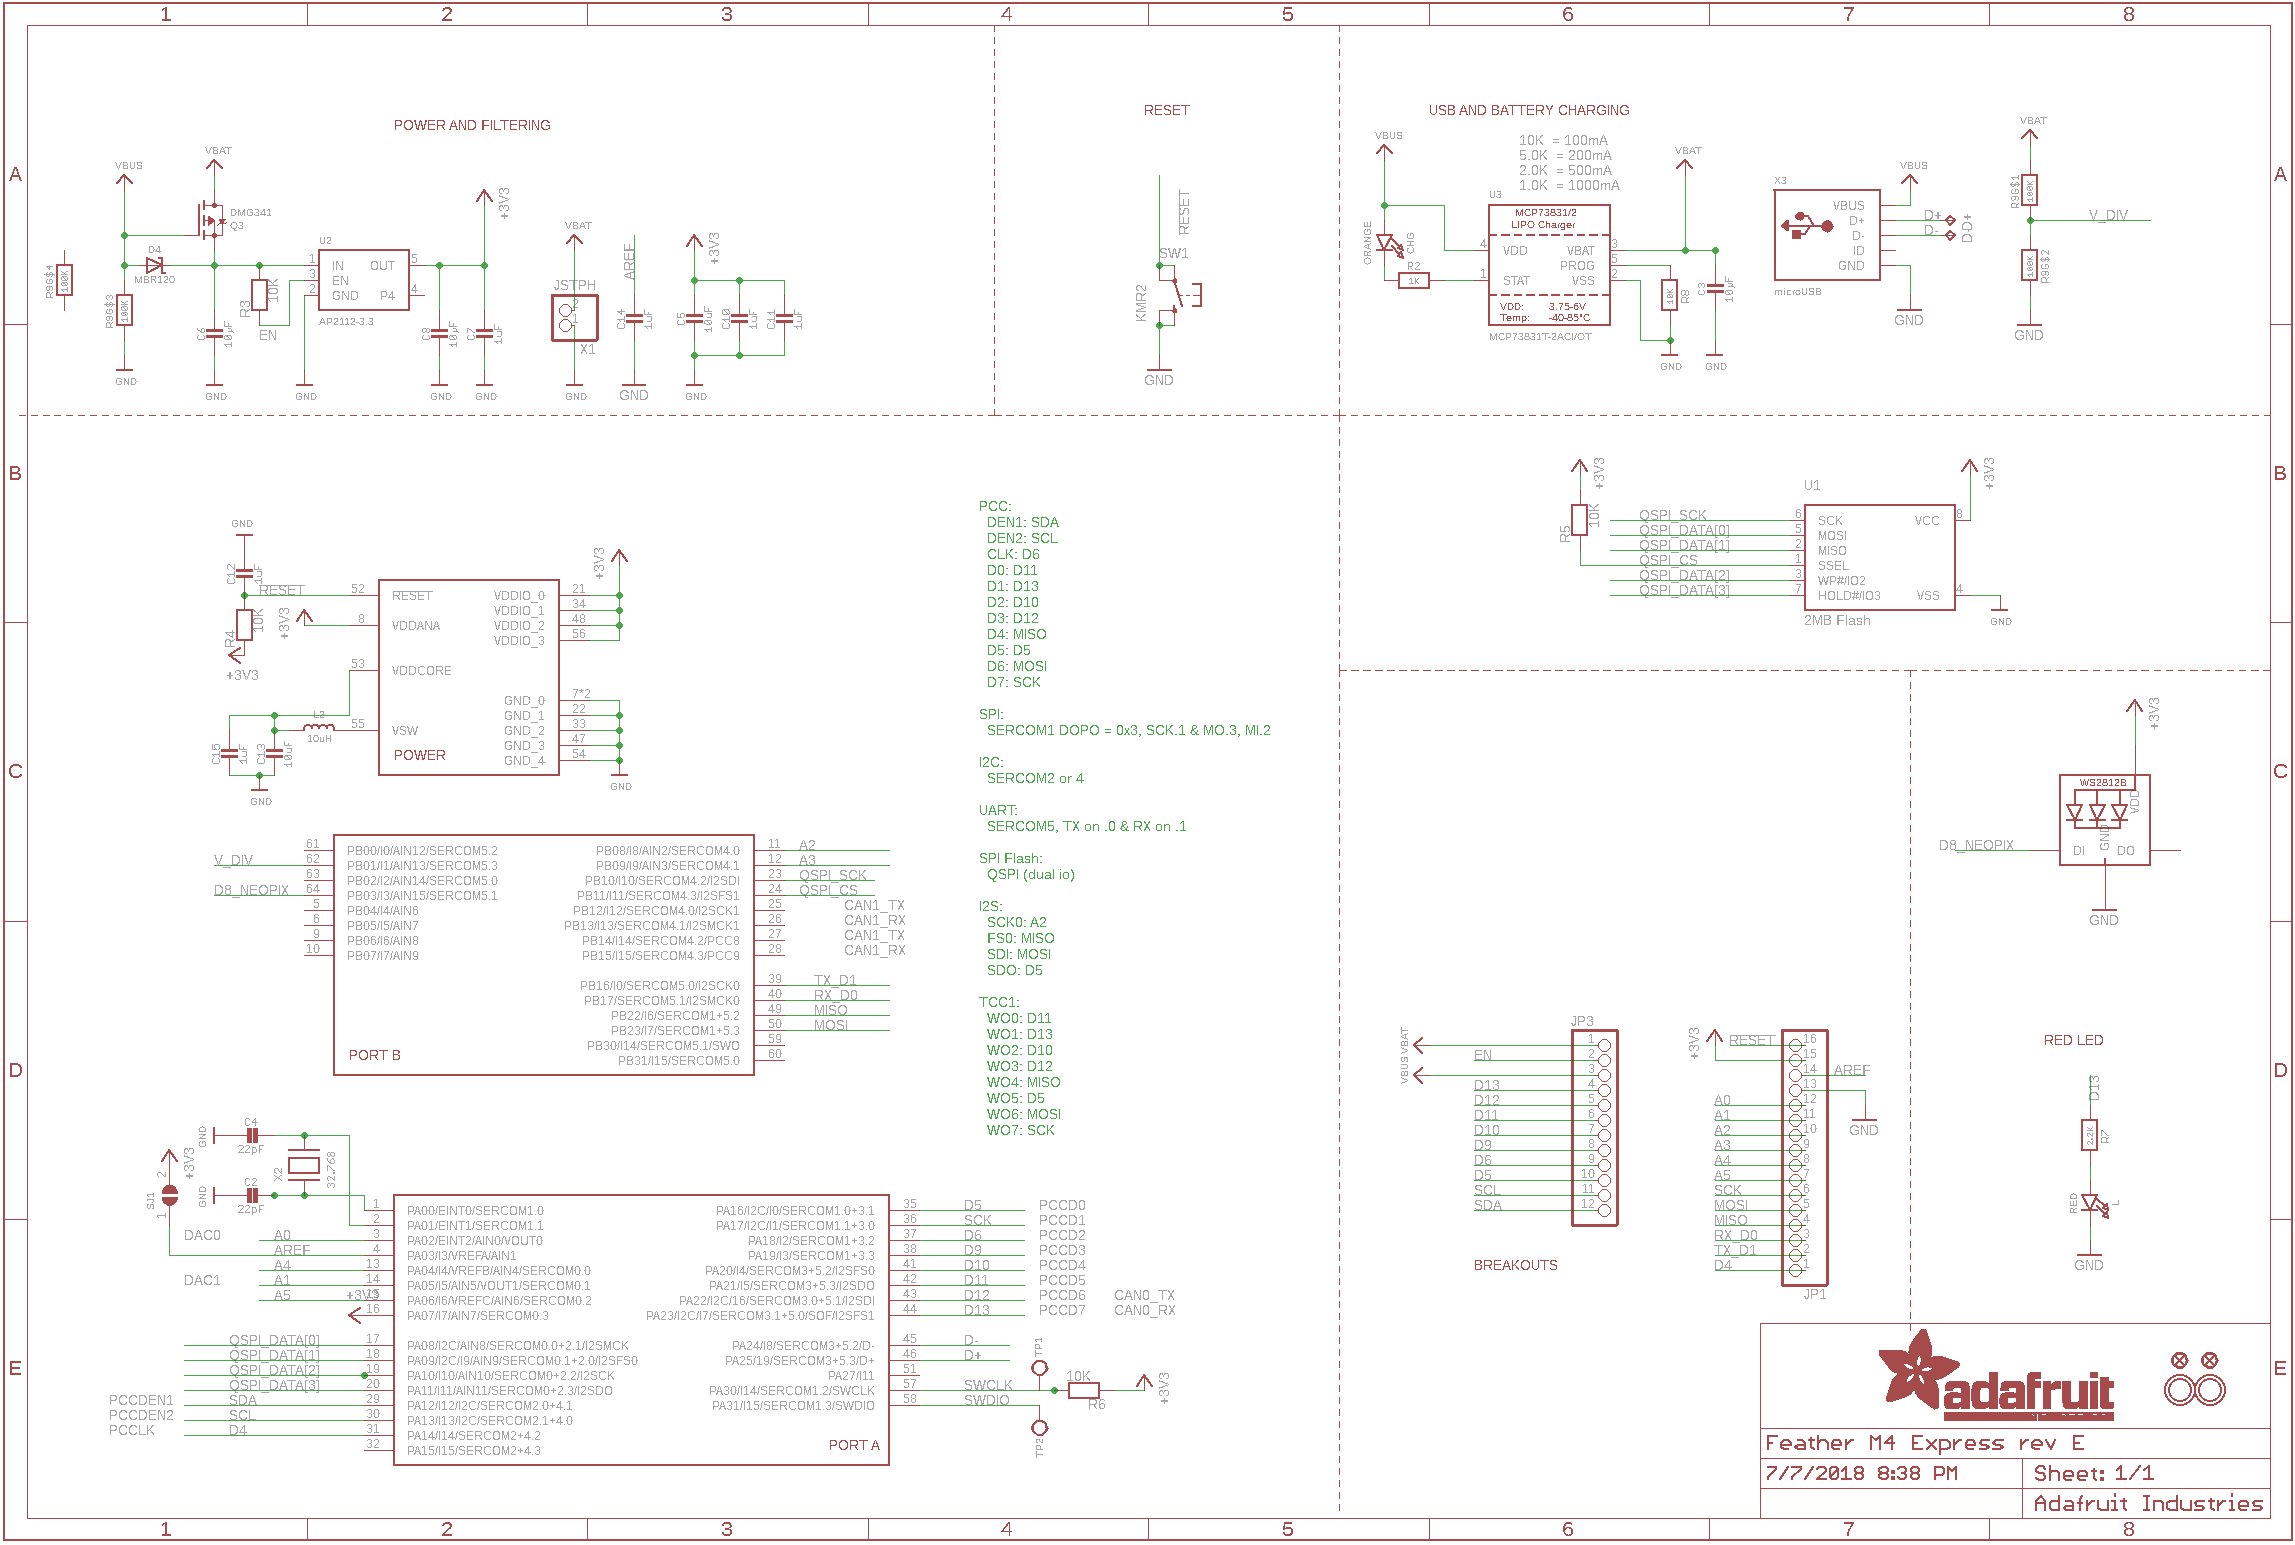
\includegraphics[width=\textwidth]{images/adafruit_featherm4_schematic}
	\caption{Feather M4 Express schematic, used in the main CDH board.}
	\label{fig:schematic-featherm4}
\end{figure}
\begin{figure}[H]
	\centering
	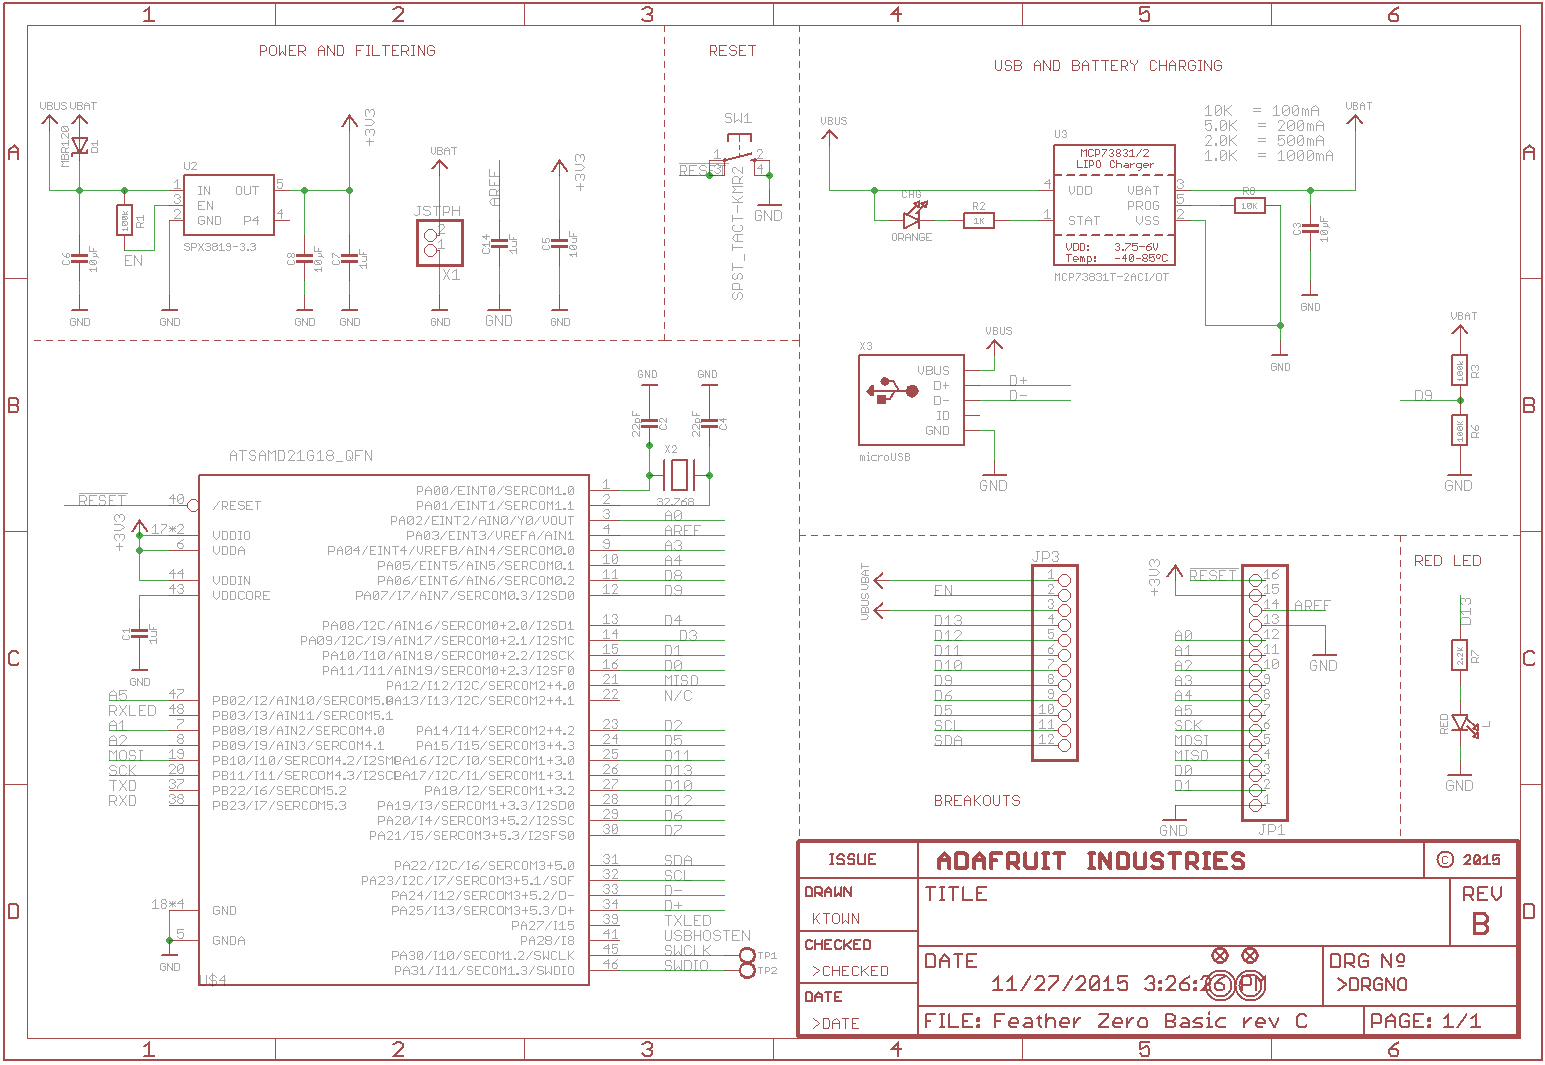
\includegraphics[width=\textwidth]{images/adafruit_featherm0_schematic}
	\caption{Feather M0 schematic, used in the IMU logger and TPM boards.}
	\label{fig:schematic-featherm0}
\end{figure}



\newpage
\subsection{TC to Digital Schematics}
Figures \ref{fig:schematic-tc-breakout-p1} and \ref{fig:schematic-tc-breakout-p2} show the schematics of the 6 channel TC to digital converter breakout board.
\begin{figure}[H]
	\centering
	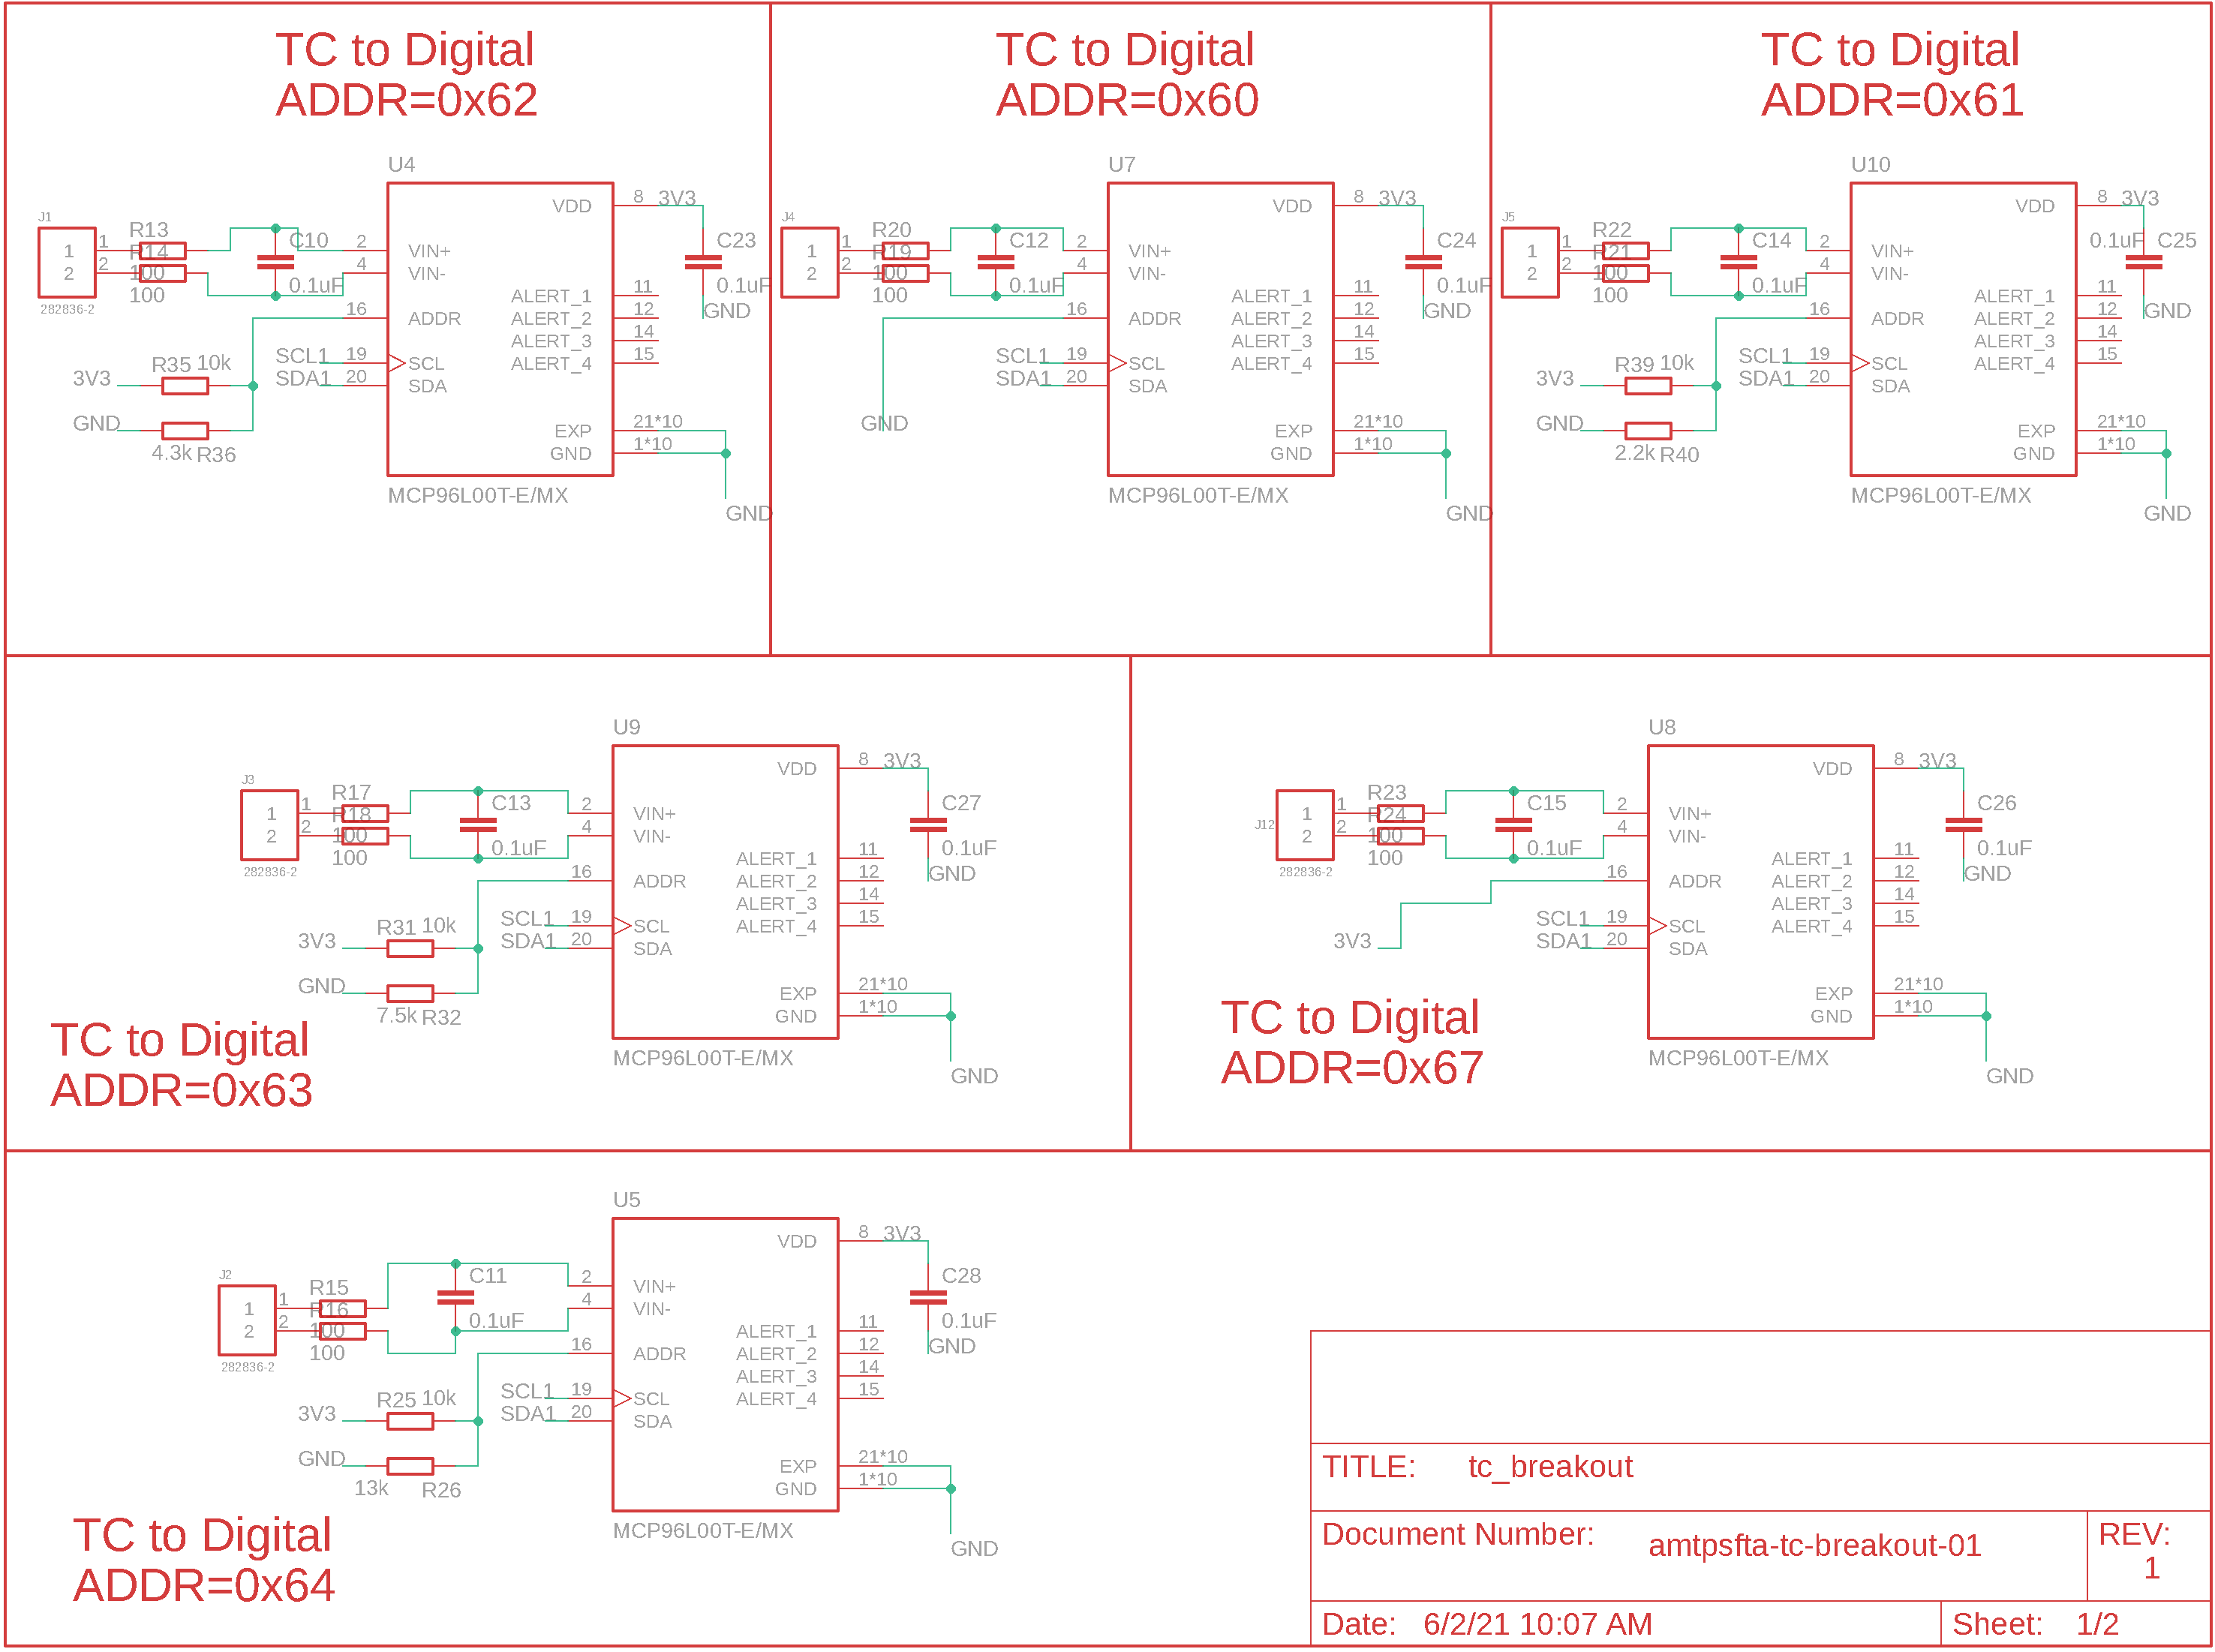
\includegraphics[width=\textwidth]{images/tc-breakout-p1}
	\caption{TC to digital schematics, page 1/2}
	\label{fig:schematic-tc-breakout-p1}
\end{figure}

\begin{figure}[H]
	\centering
	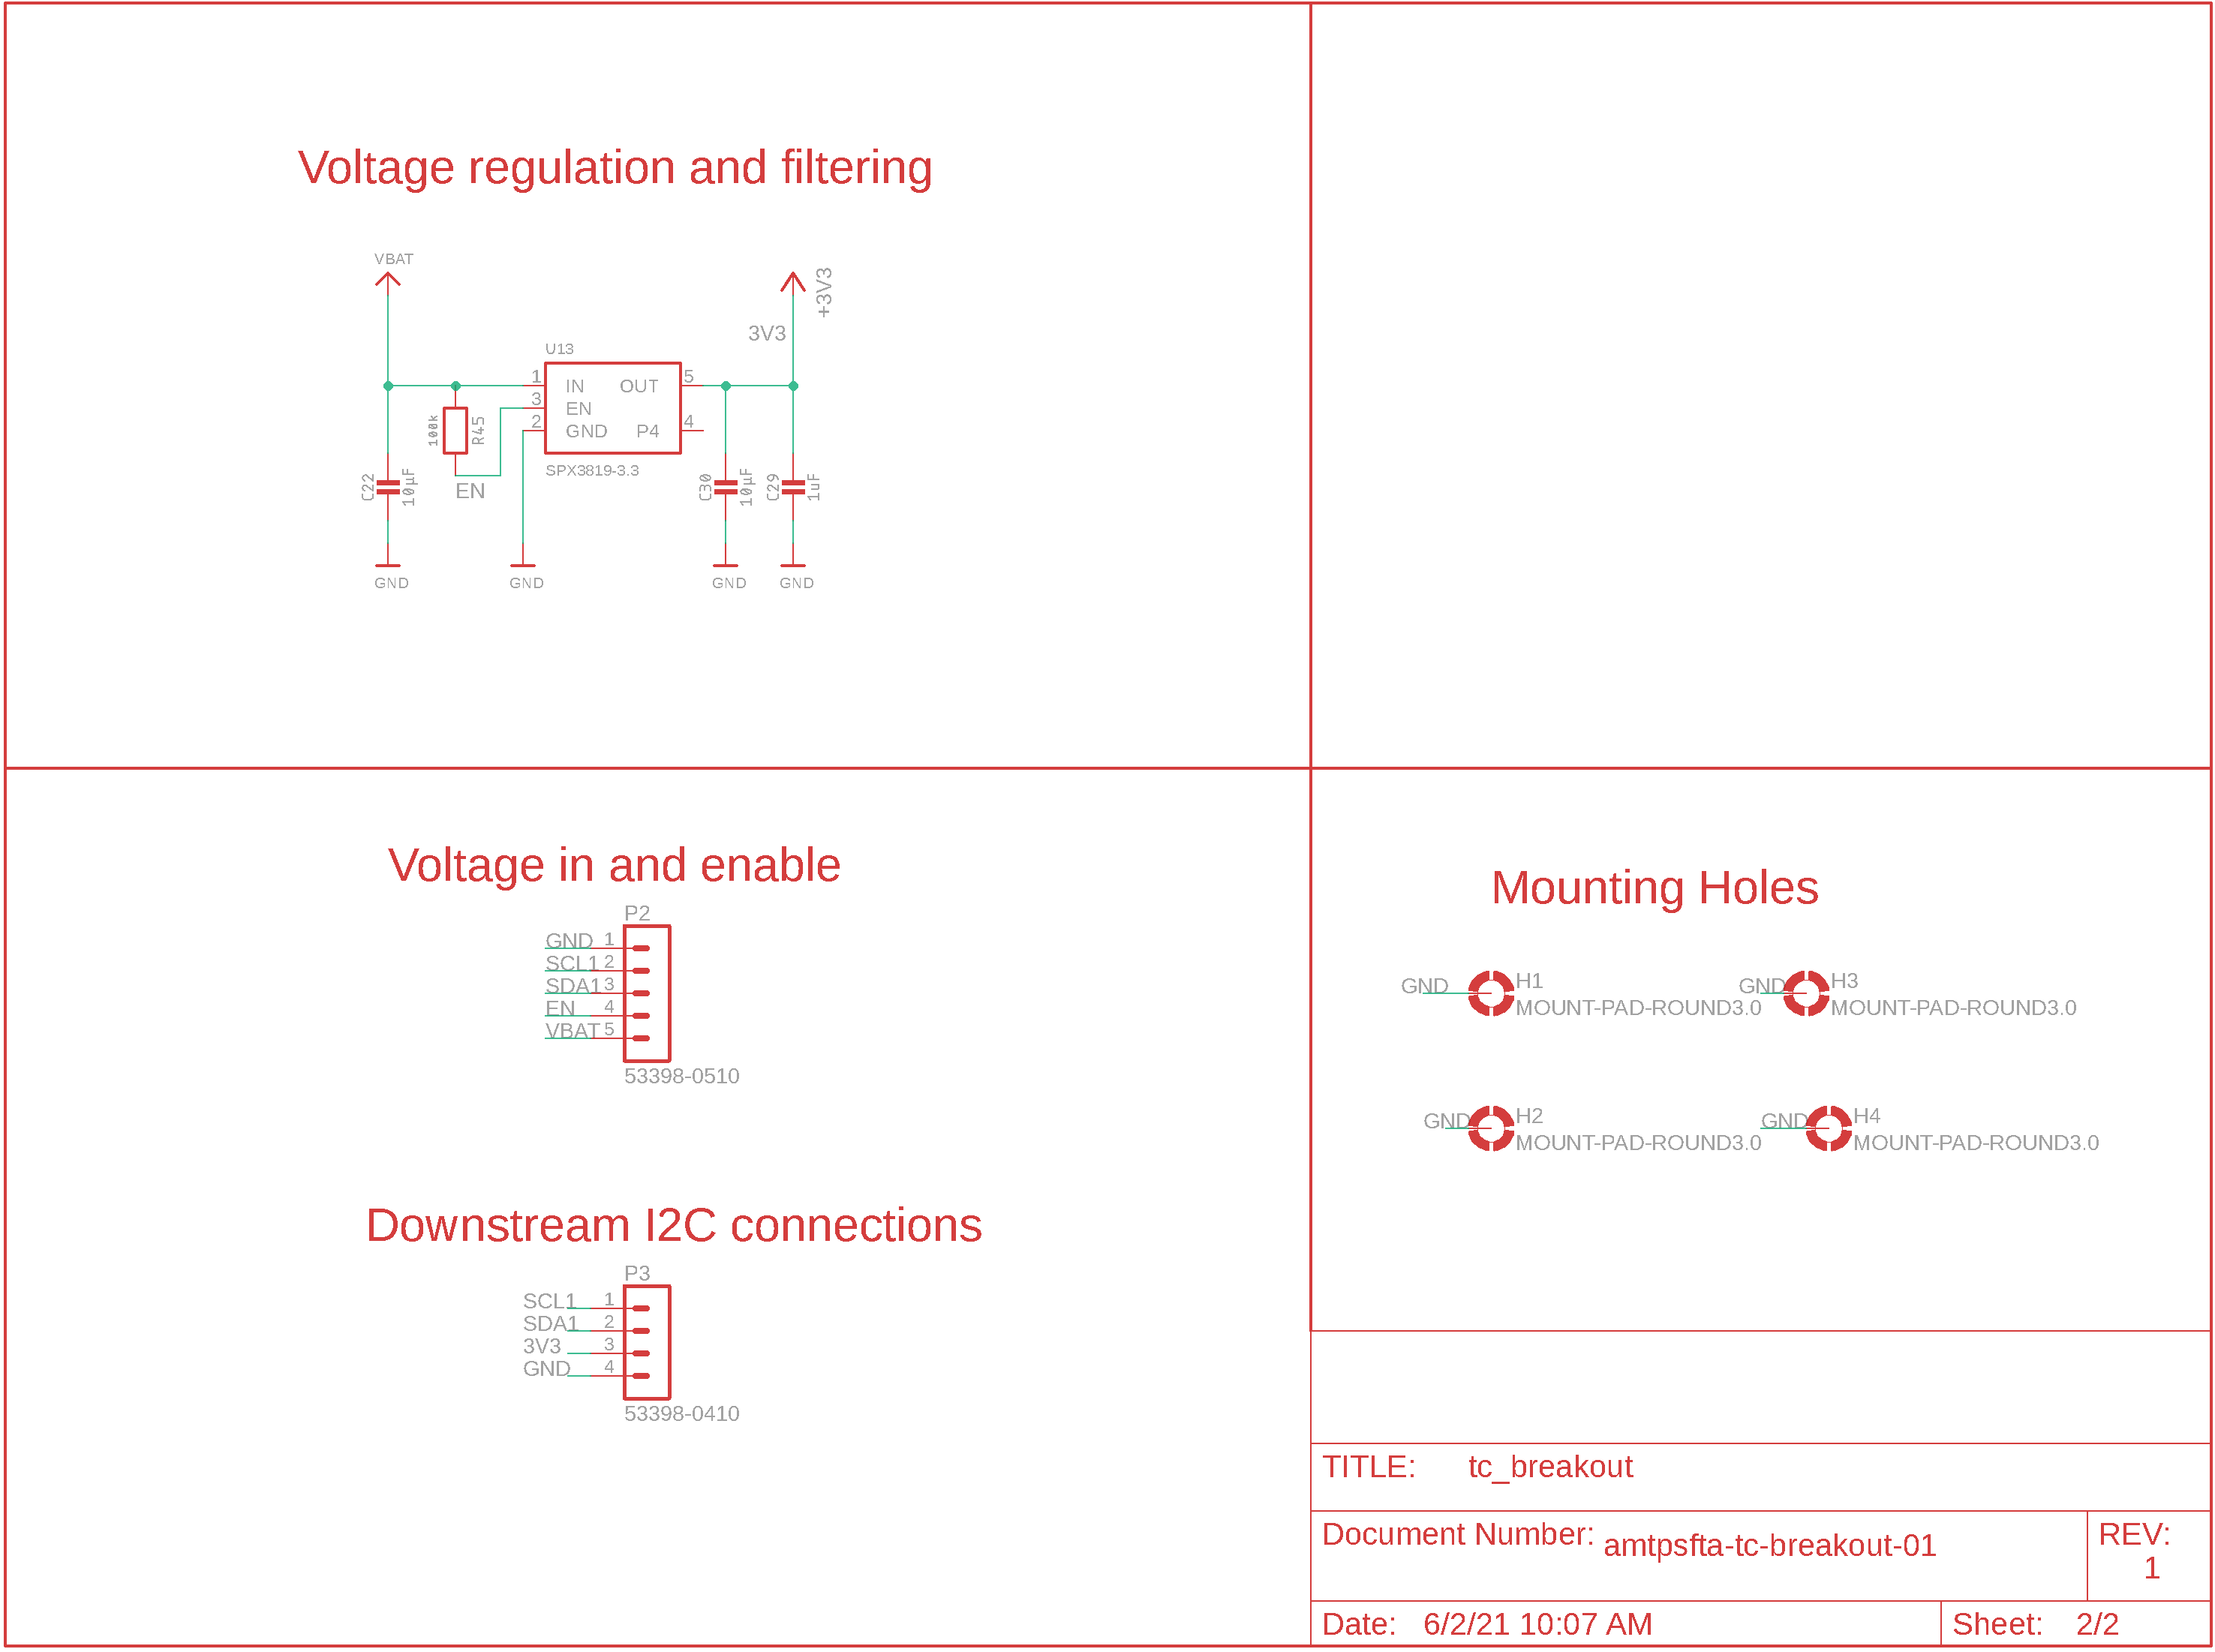
\includegraphics[width=\textwidth]{images/tc-breakout-p2}
	\caption{TC to digital schematics, page 2/2}
	\label{fig:schematic-tc-breakout-p2}
\end{figure}



\newpage
\subsection{Main CDH Schematics}
Figures \ref{fig:schematic-cdh-p1} and \ref{fig:schematic-cdh-p2} show the schematics of the main CDH PCB.
\begin{figure}[H]
	\centering
	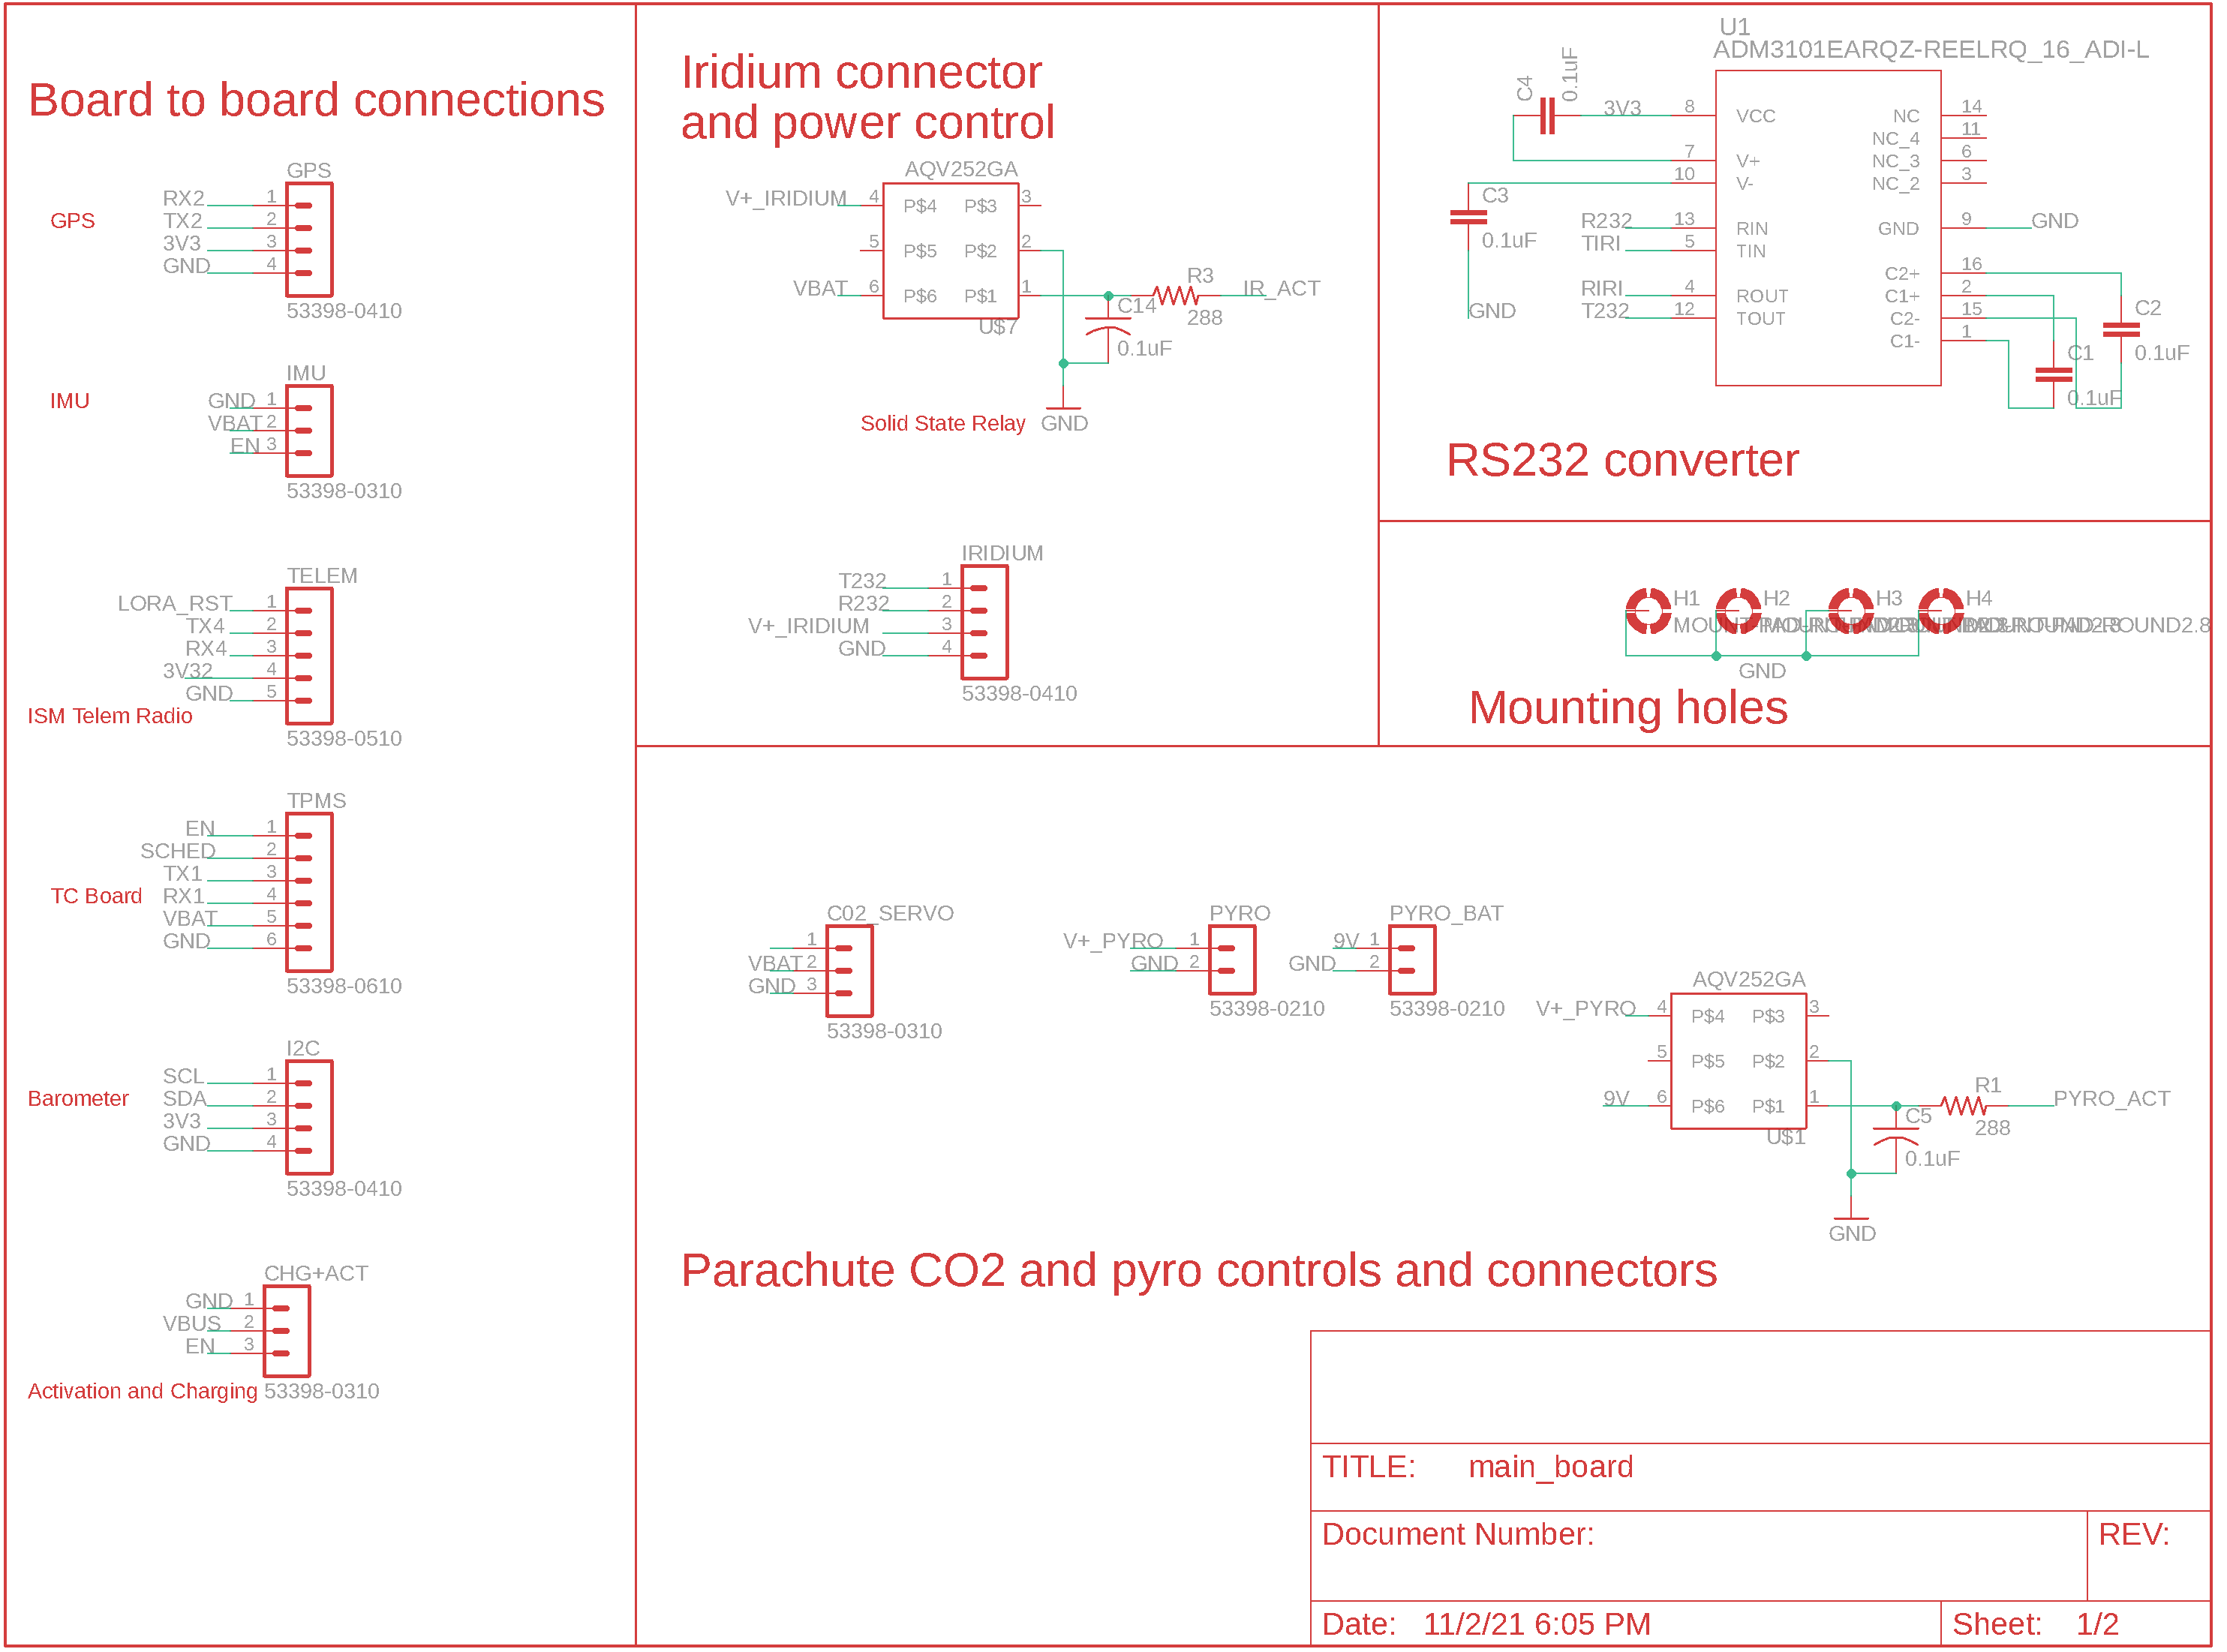
\includegraphics[width=\textwidth]{images/main_board_schem_1}
	\caption{Main CDH schematics, page 1/2}
	\label{fig:schematic-cdh-p1}
\end{figure}
\begin{figure}[H]
	\centering
	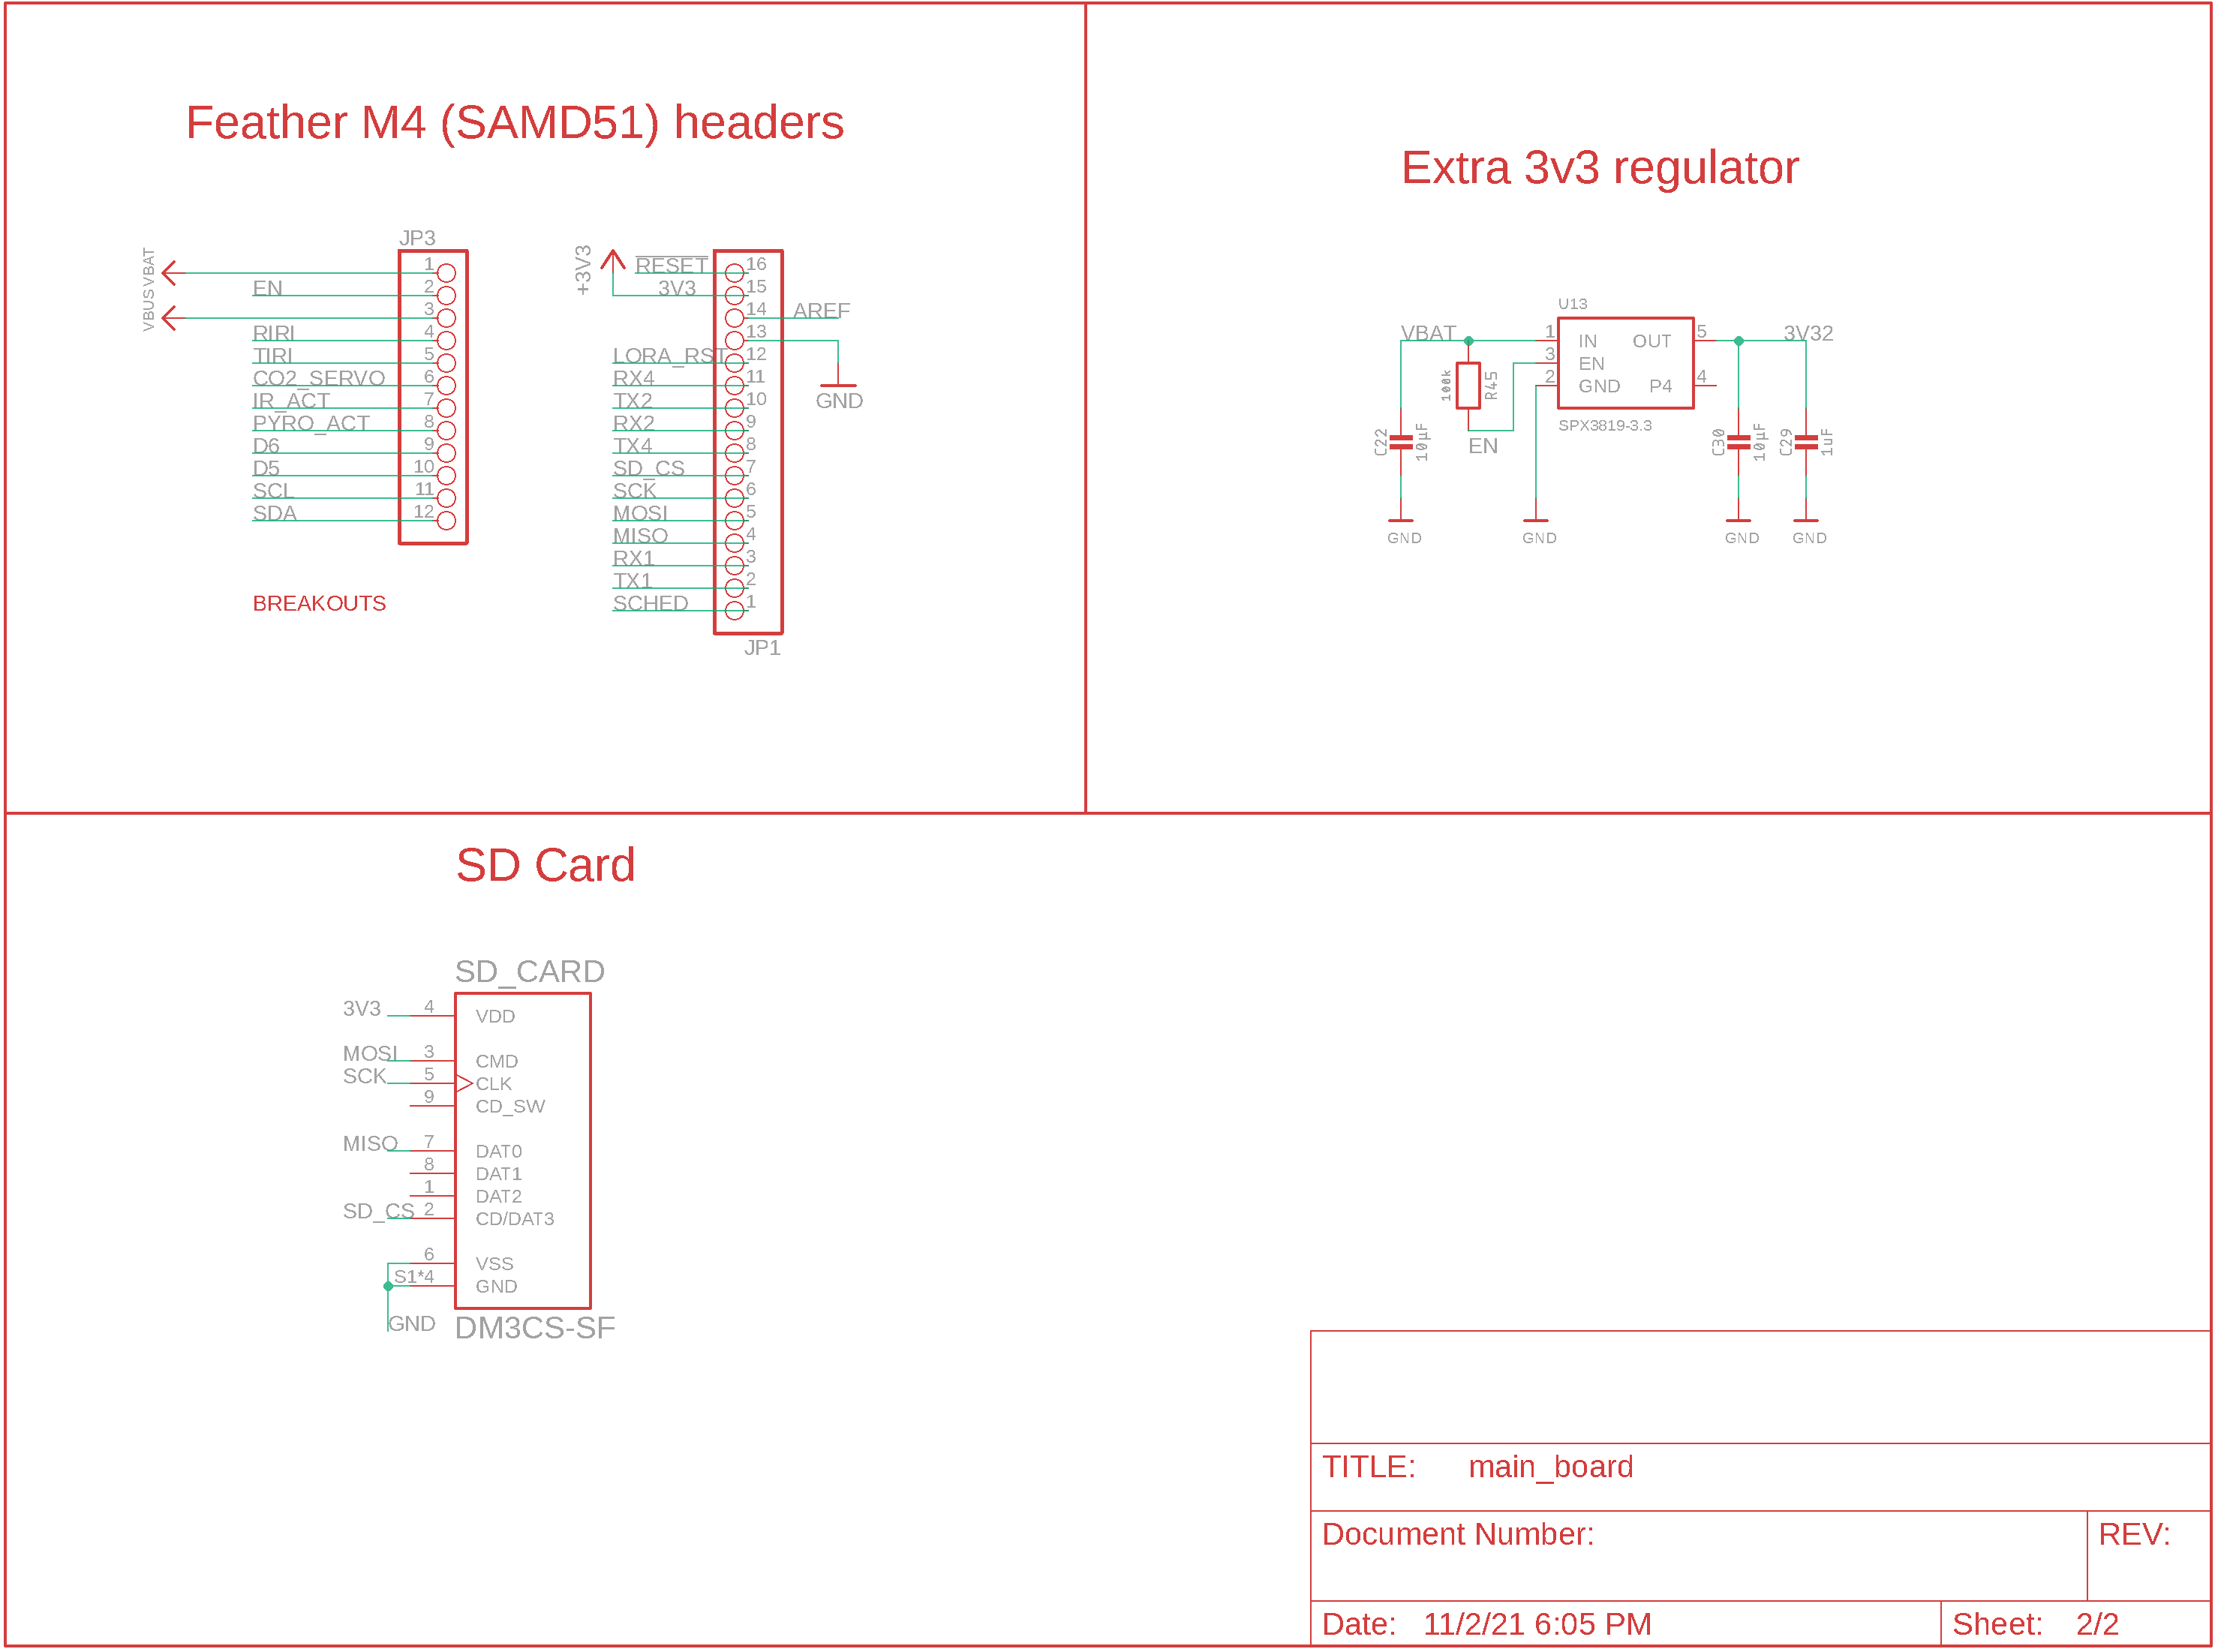
\includegraphics[width=\textwidth]{images/main_board_schem_2}
	\caption{Main CDH schematics, page 2/2}
	\label{fig:schematic-cdh-p2}
\end{figure}


\newpage
\subsection{TPM Schematics}
Figures \ref{fig:schematic-tpm-p1} and \ref{fig:schematic-tpm-p2} show the schematics of the TPM subsystem PCB.
\begin{figure}[H]
	\centering
	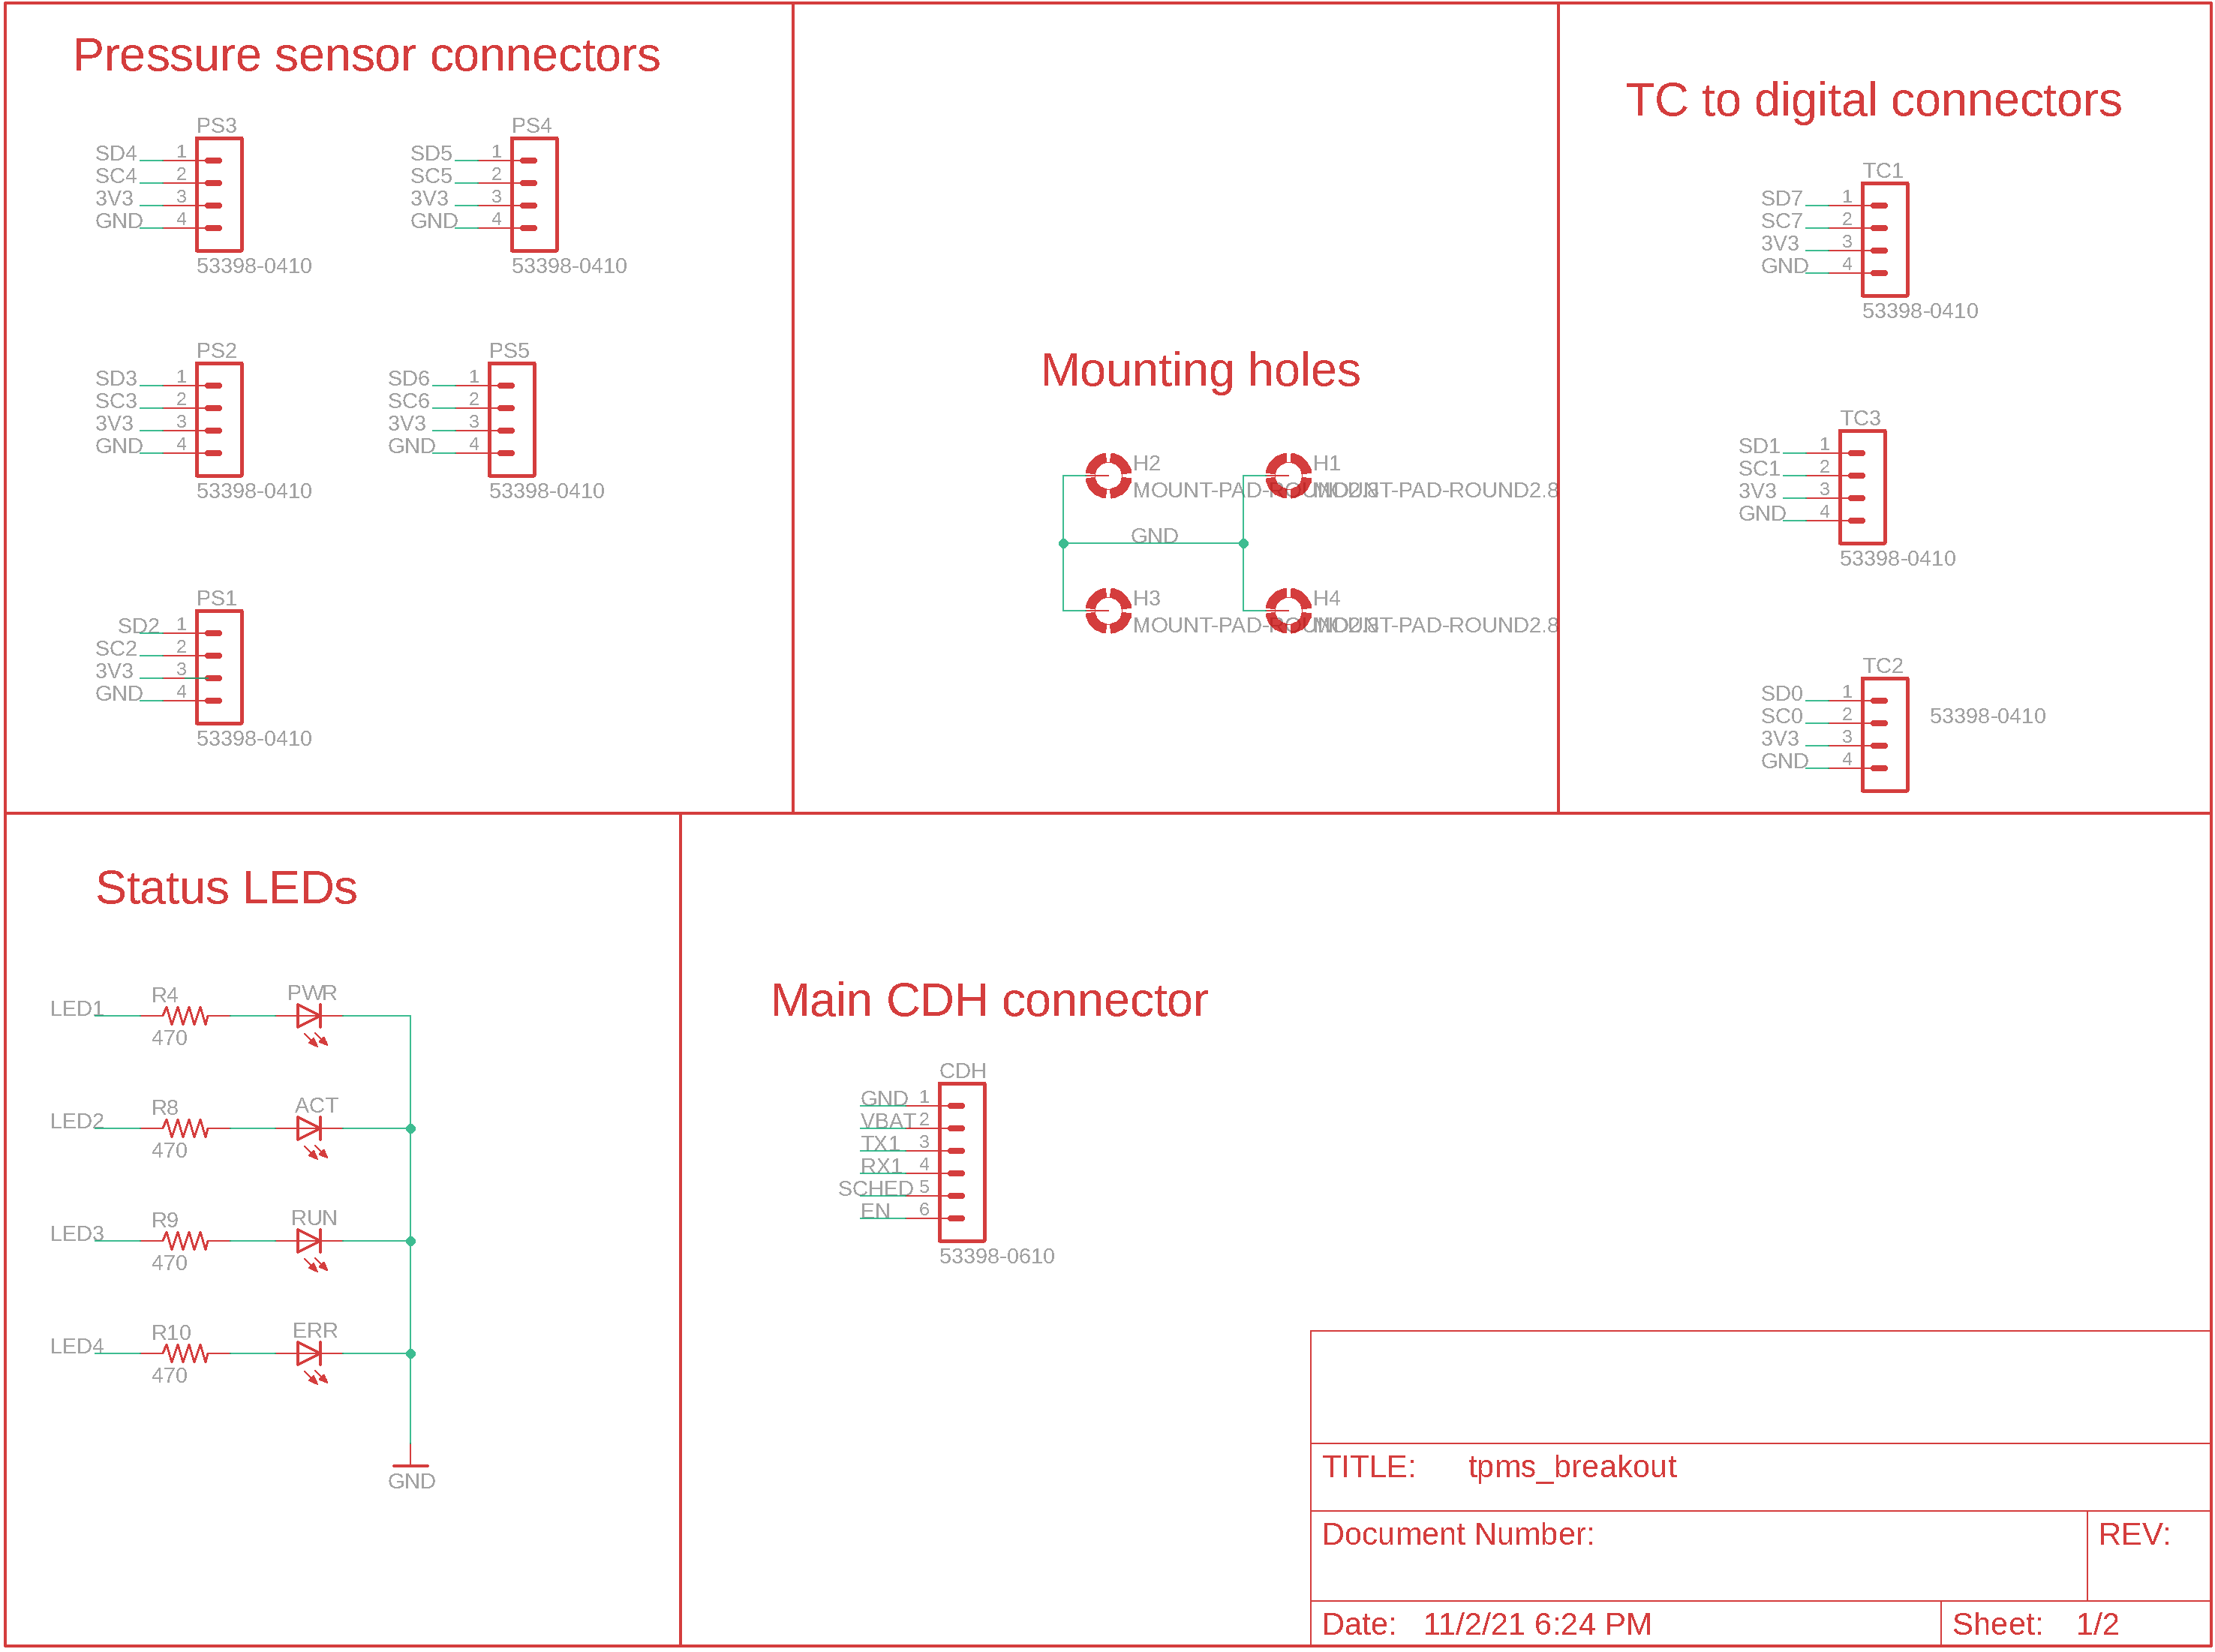
\includegraphics[width=\textwidth]{images/tpms_breakout_schem_1}
	\caption{TPM schematics, page 1/2}
	\label{fig:schematic-tpm-p1}
\end{figure}
\begin{figure}[H]
	\centering
	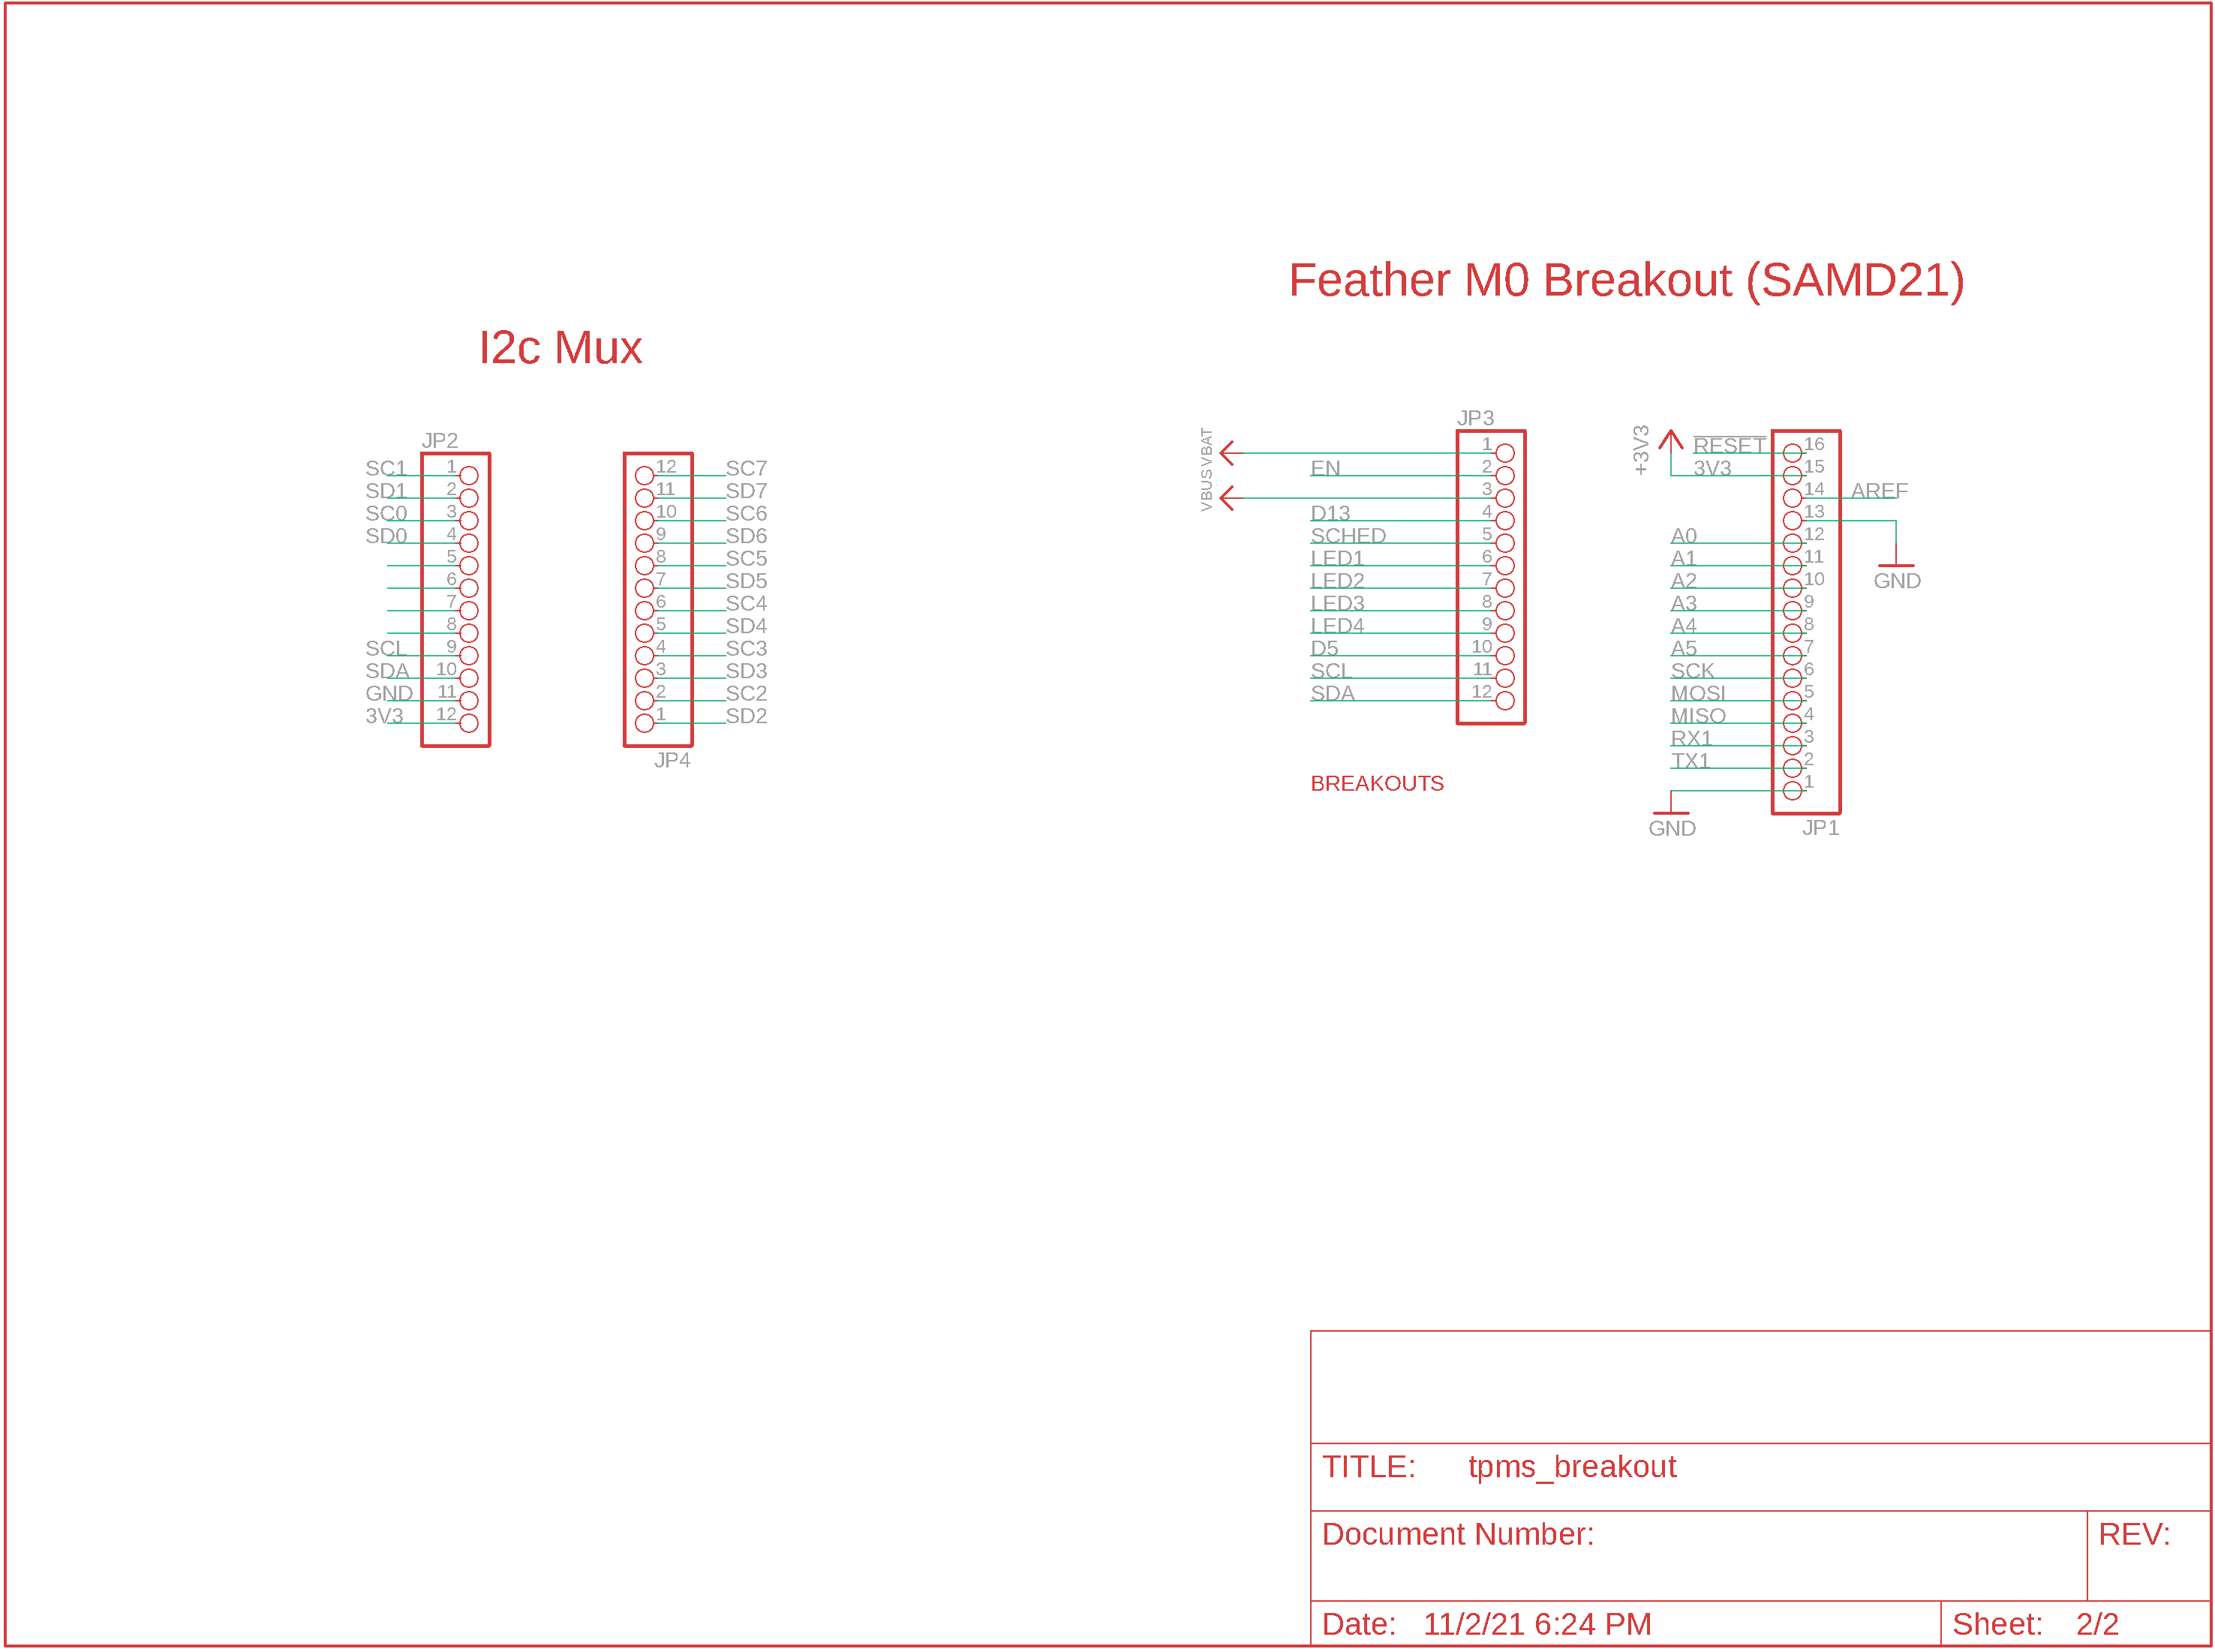
\includegraphics[width=\textwidth]{images/tpms_breakout_schem_2}
	\caption{TPM schematics, page 2/2}
	\label{fig:schematic-tpm-p2}
\end{figure}


\newpage
\subsection{IMU Logger Schematics}
Figures \ref{fig:schematic-imu-p1}, \ref{fig:schematic-imu-p2}, and \ref{fig:schematic-imu-p3} show the schematics of the IMU logger PCB.
\begin{figure}[H]
	\centering
	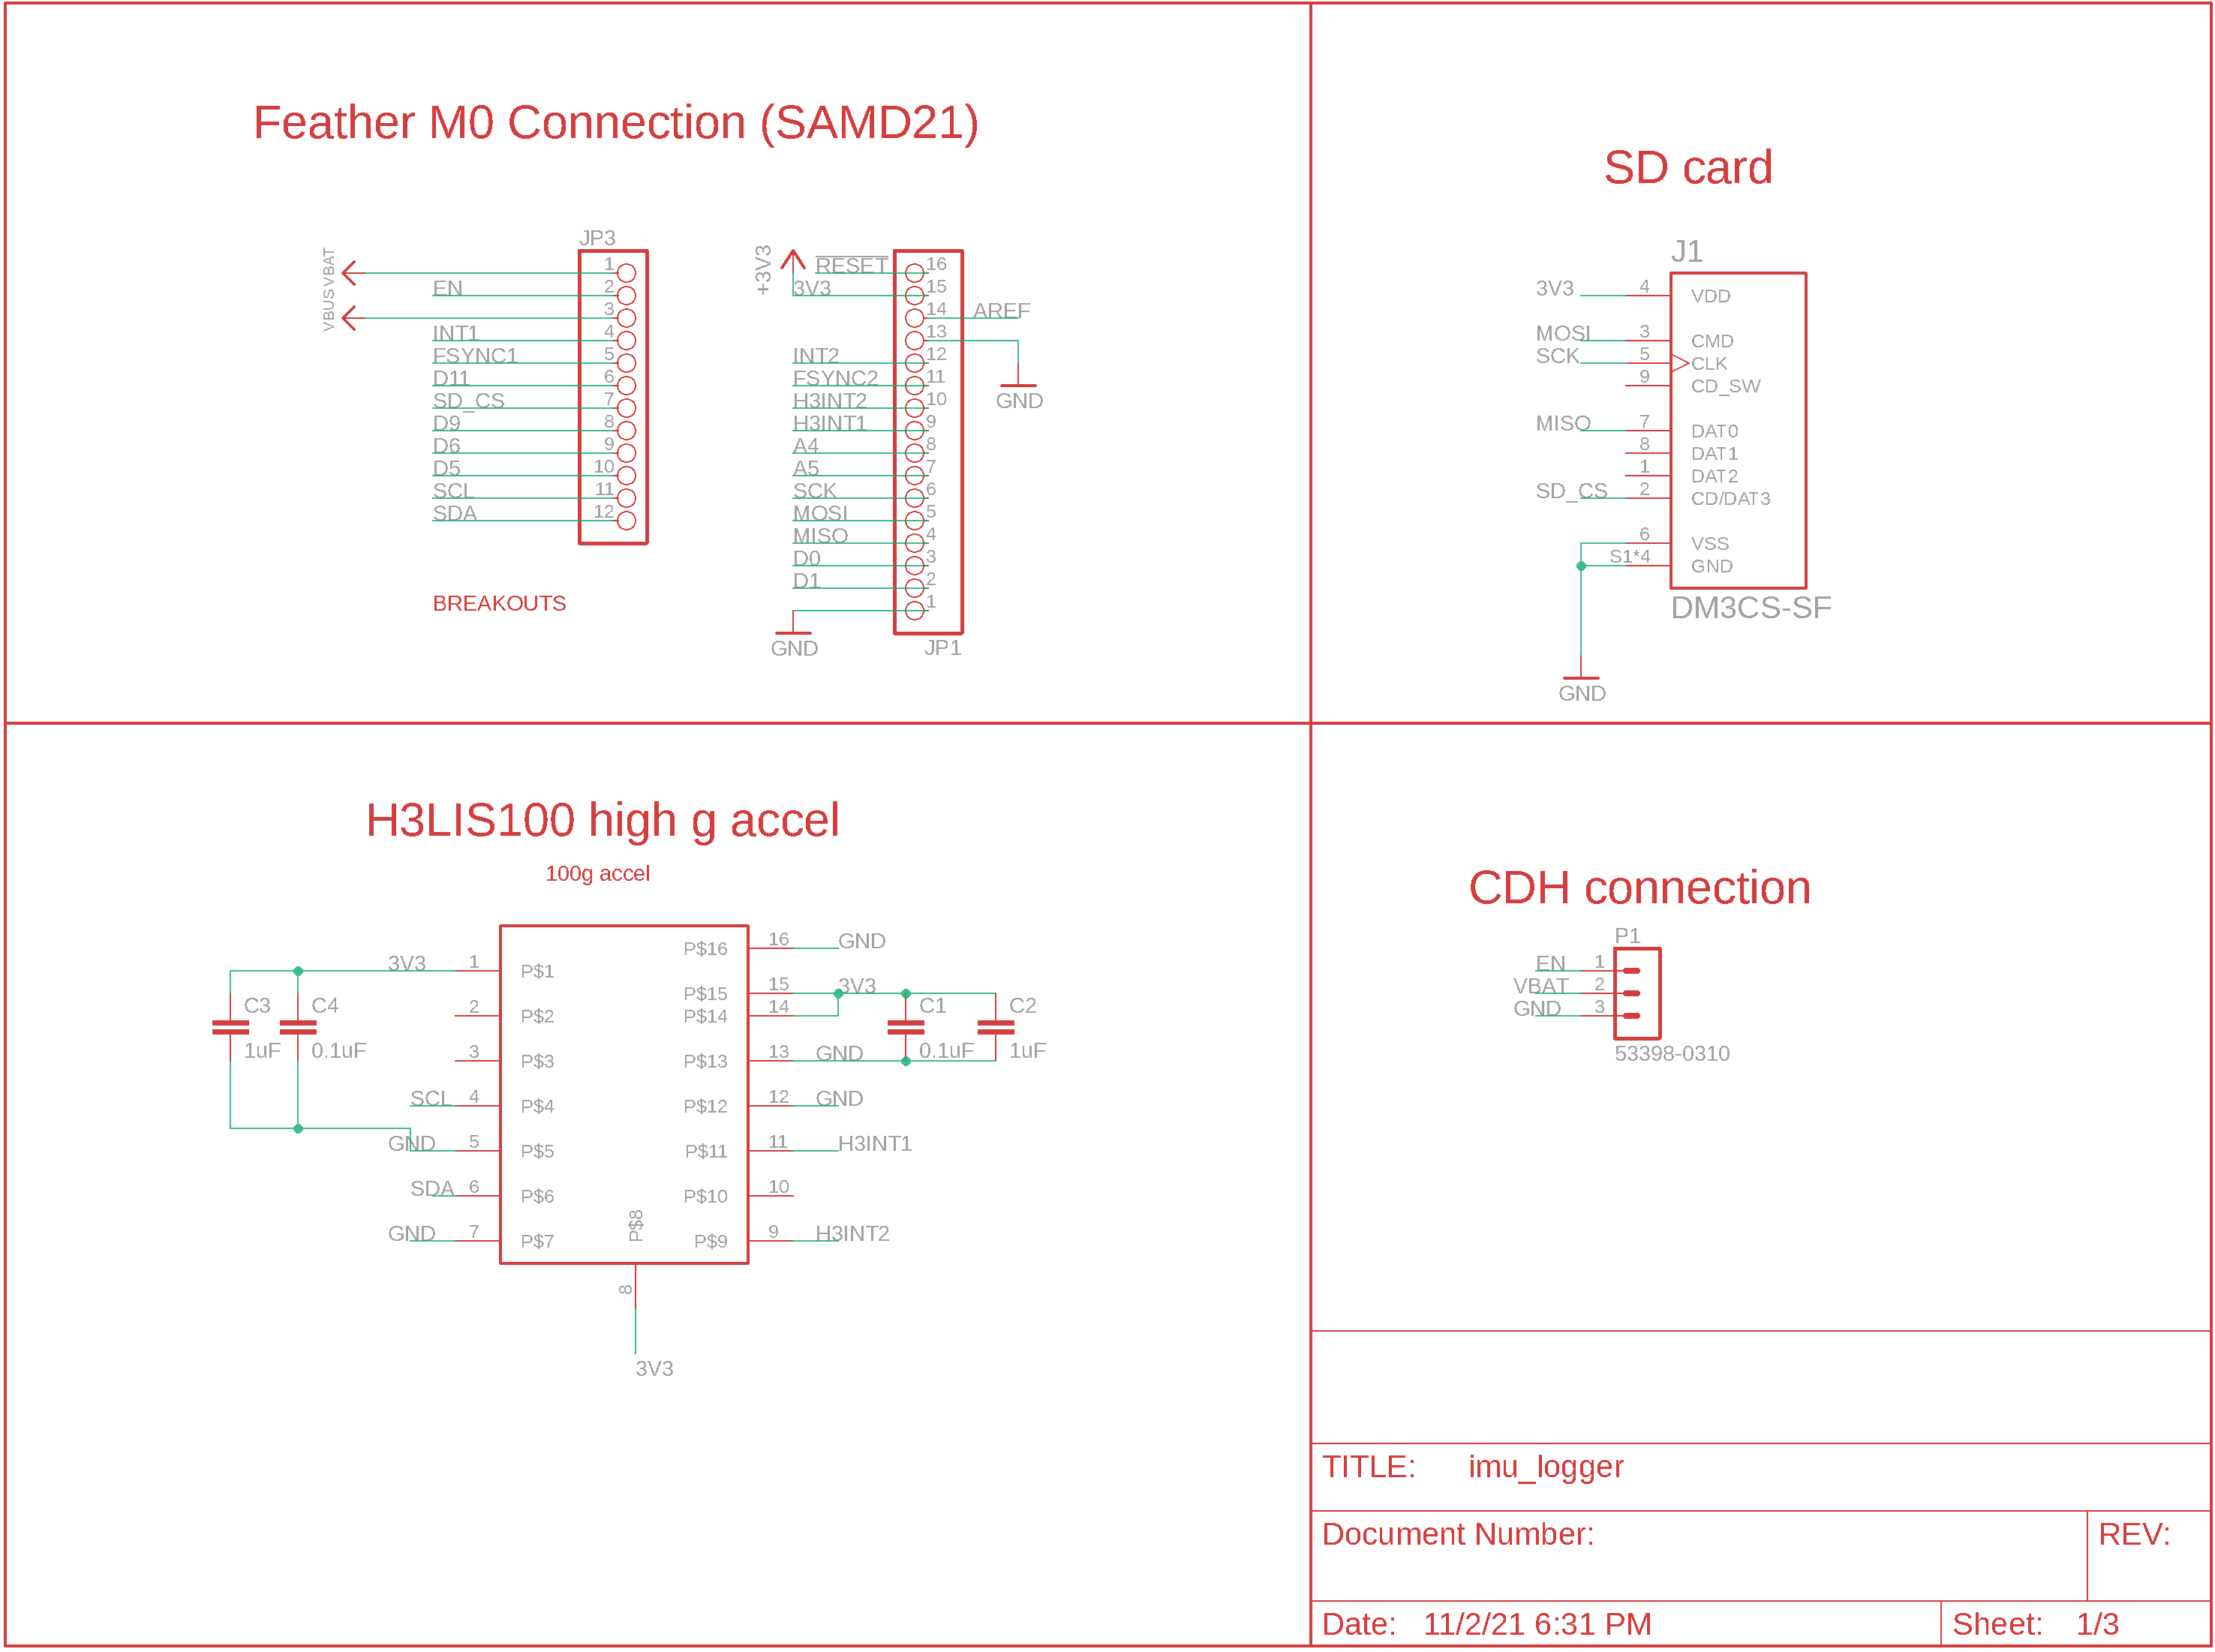
\includegraphics[width=\textwidth]{images/imu_logger_schem_1}
	\caption{IMU logger schematics, page 1/3}
	\label{fig:schematic-imu-p1}
\end{figure}
\begin{figure}[H]
	\centering
	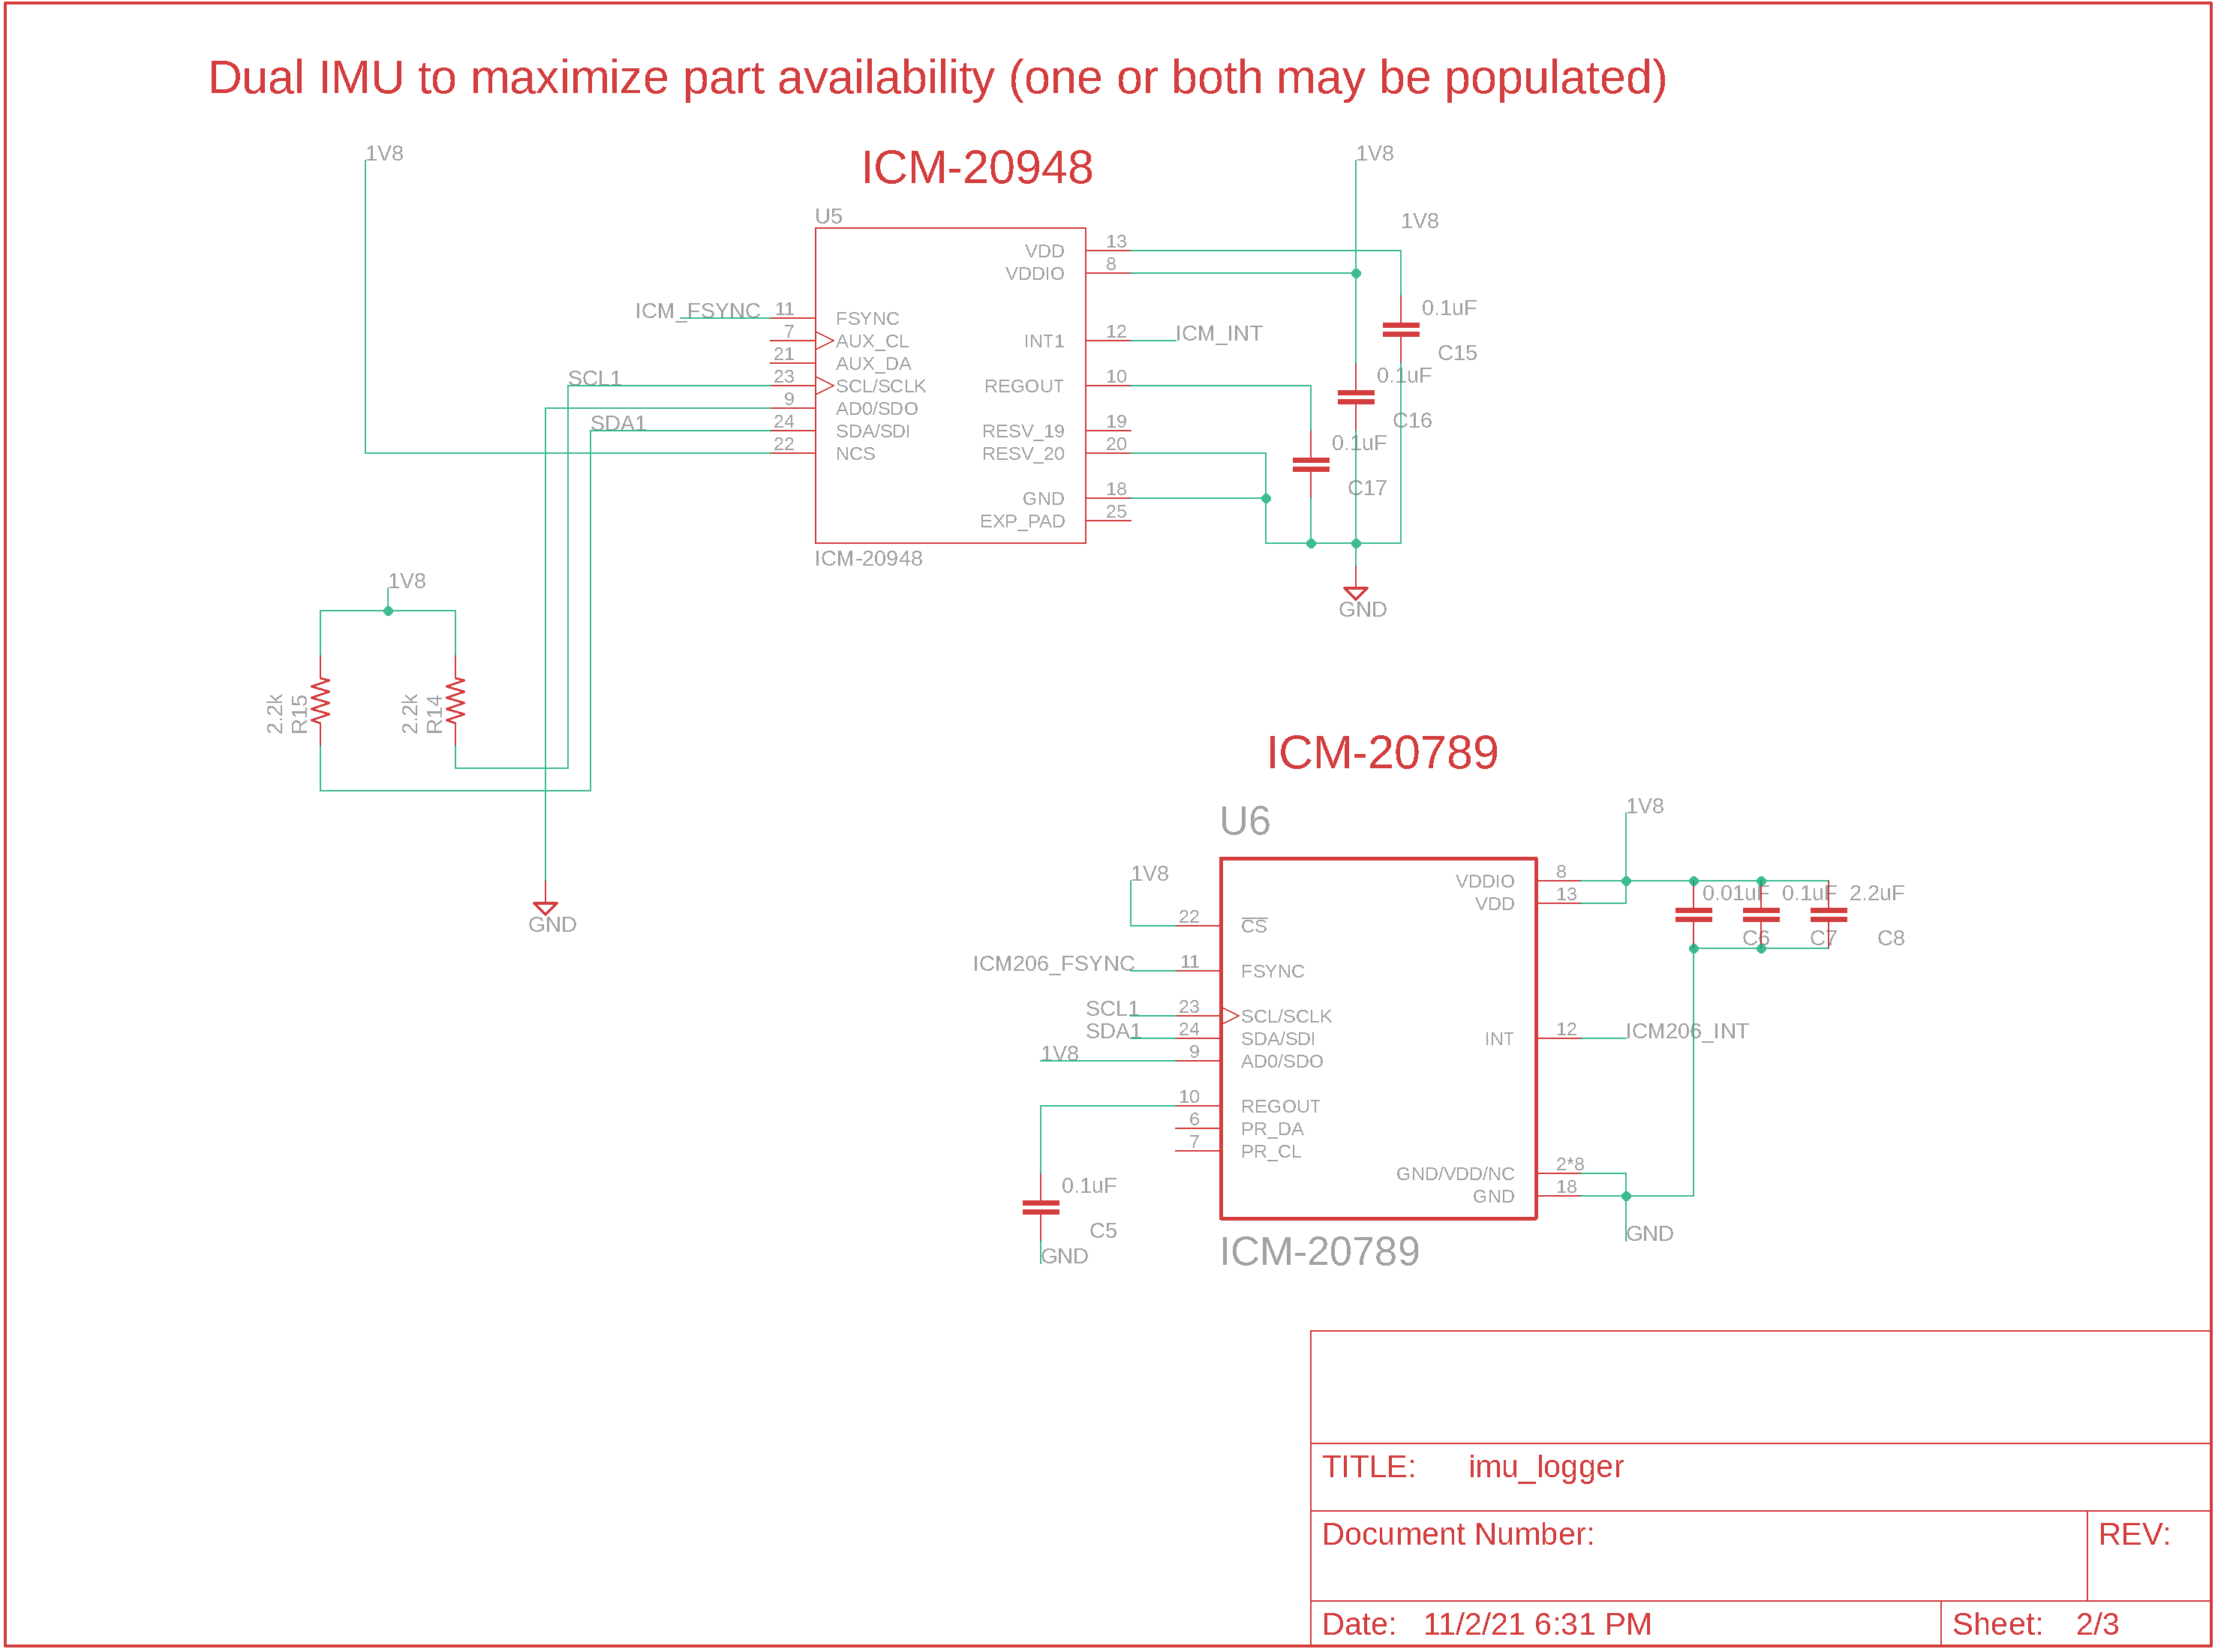
\includegraphics[width=\textwidth]{images/imu_logger_schem_2}
	\caption{IMU logger schematics, page 2/3}
	\label{fig:schematic-imu-p2}
\end{figure}
\begin{figure}[H]
	\centering
	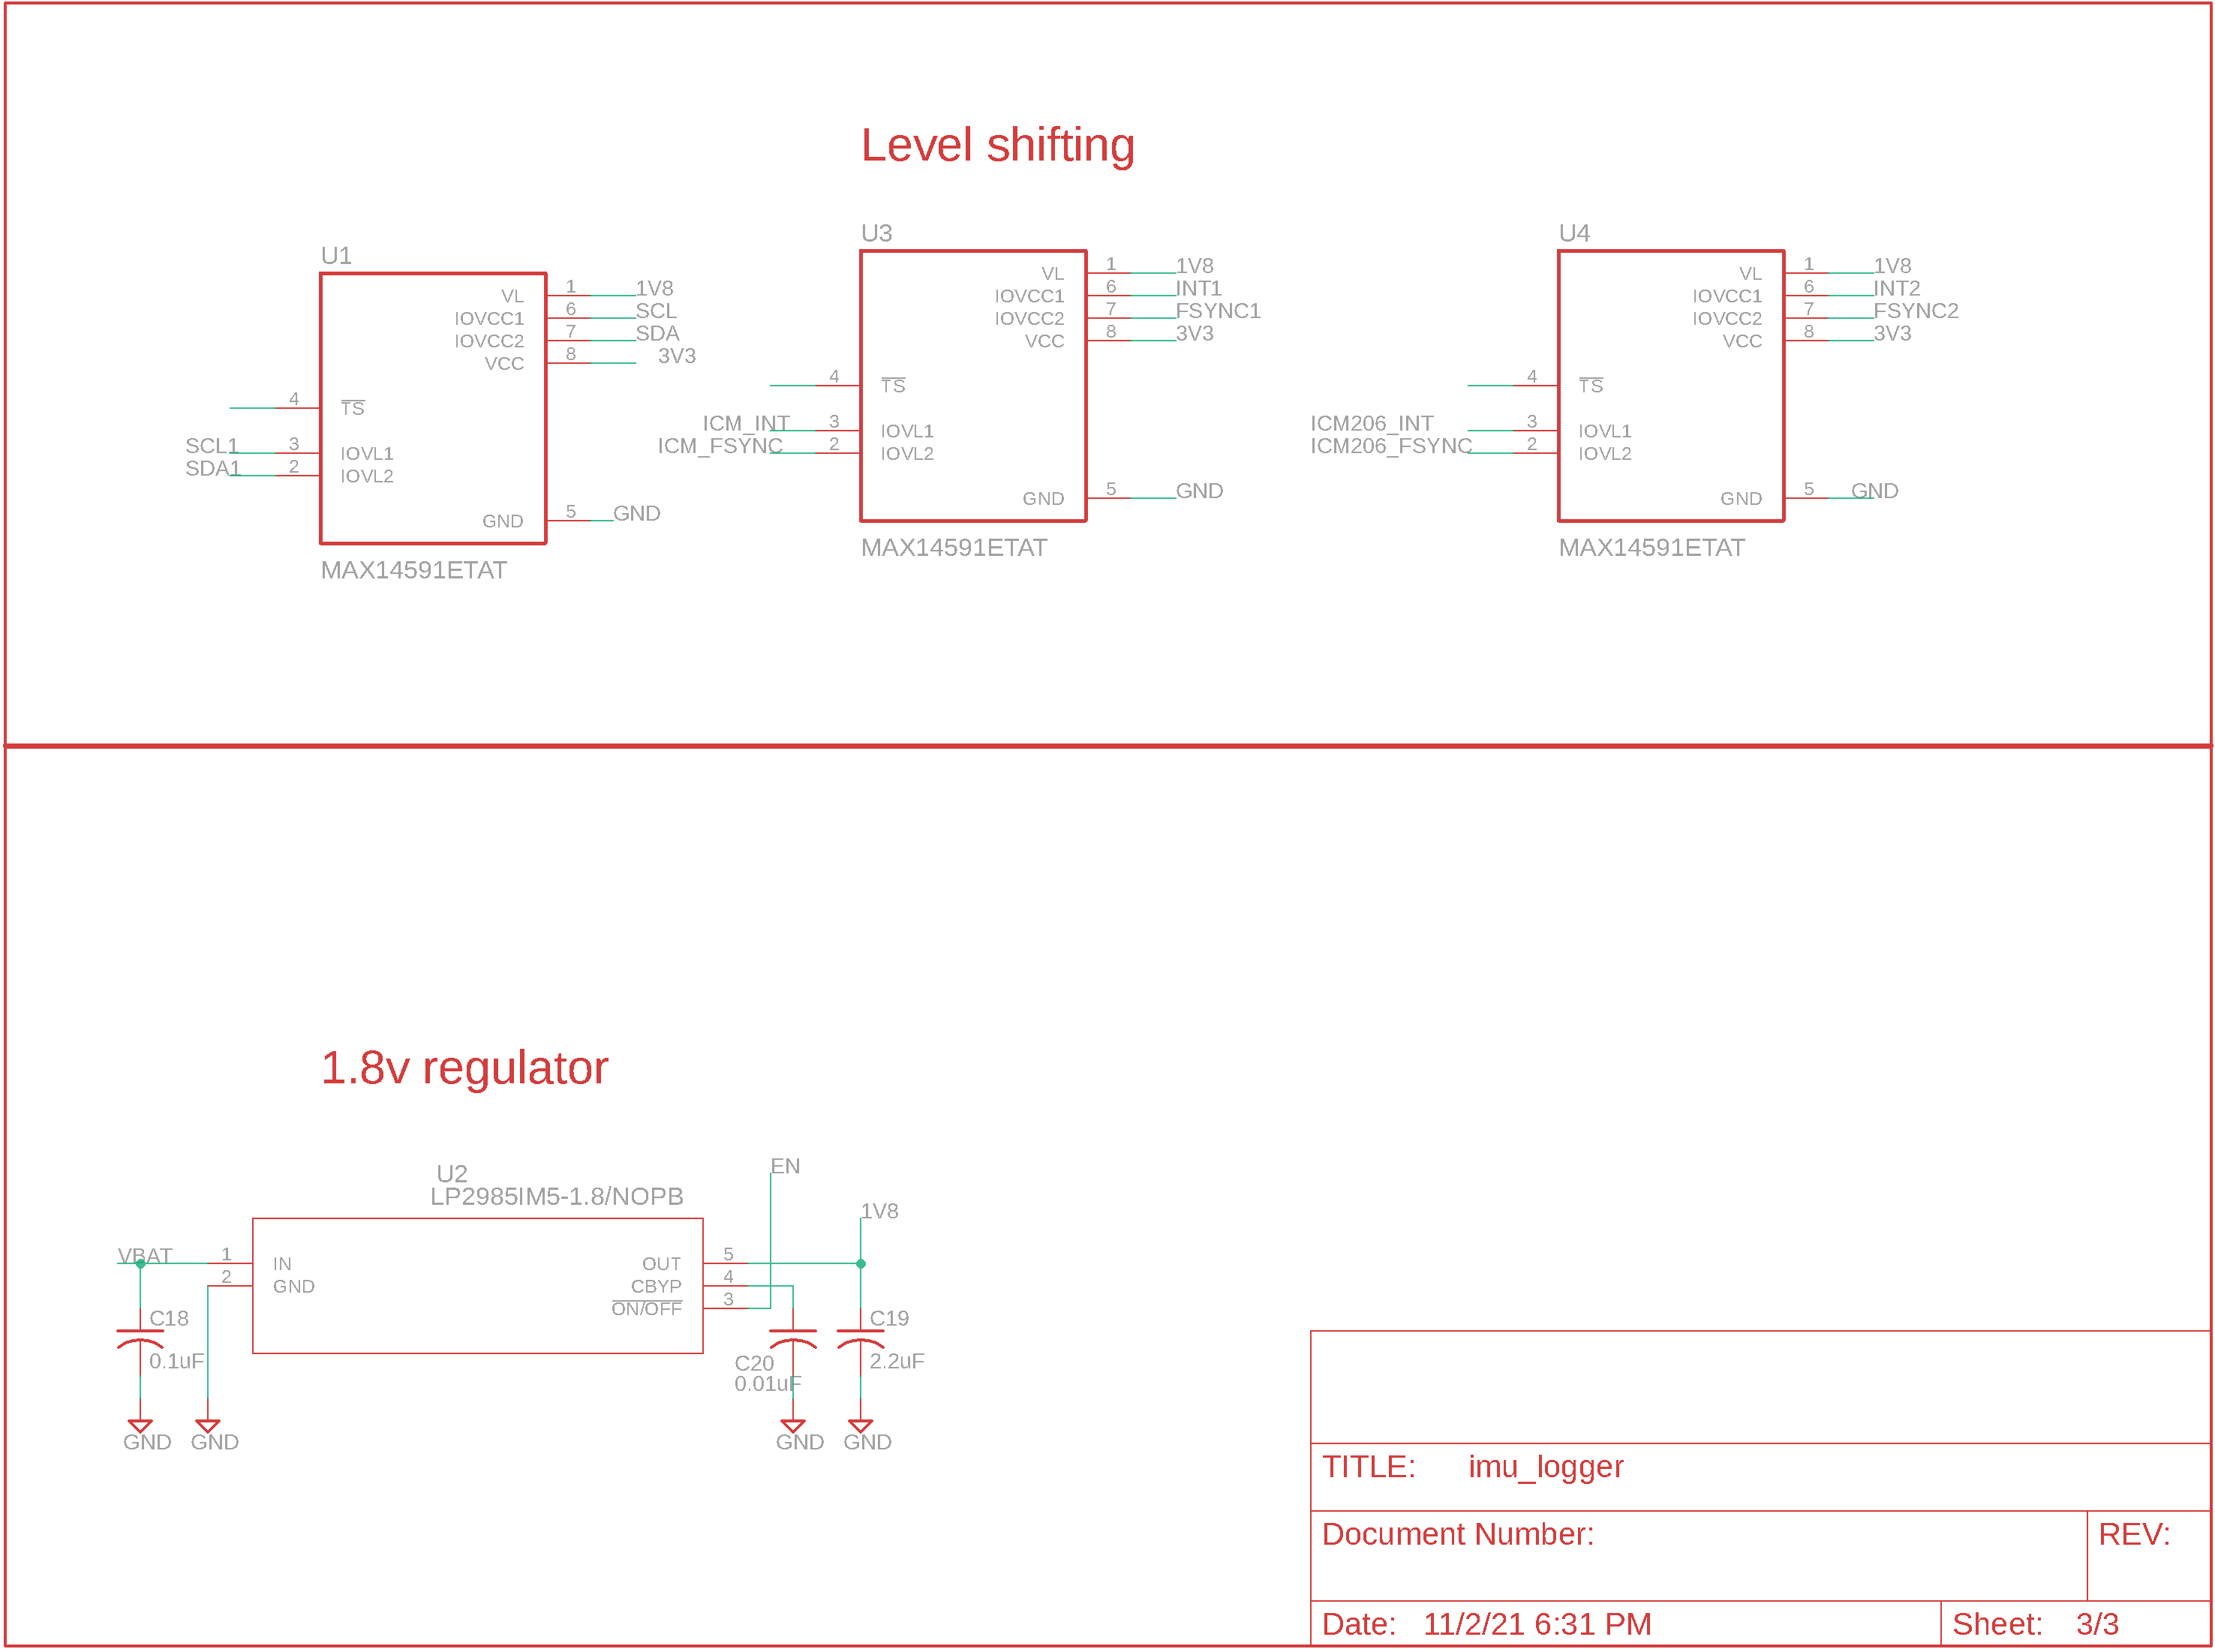
\includegraphics[width=\textwidth]{images/imu_logger_schem_3}
	\caption{Page 3/3}
	\label{fig:schematic-imu-p3}
\end{figure}



\newgeometry{margin=2cm} % modify this if you need even more space
\begin{landscape}
\section{Test Matrix}
\label{appendix-testing}
\begin{table}[!bp]
	\centering
		%\begin{minipage}{0.95\textheight}
			\def\arraystretch{1.75}
			\small\centering
			\setlength{\tabcolsep}{1.0mm}
			\scriptsize
			\centering
			\caption{Test matrix for avionics integration verifications}
			\label{my-label}  
			
			\begin{table}[H]
				\scriptsize
				\begin{tabular}{p{3cm} | p{13cm}  L p{5cm}}
					\textbf{Test Name} &\textbf{ Description, verification or procedure}& \textbf{ ECD / Progress} & \textbf{Problems/Notes} \\
					\hline
					IMU accuracy test &  Verify recorded axes orientation for all acceleration and inertial sensors matches documentation and that data received over the recovery data interfaces looks reasonable. &  Done &  \\
					
					Javad GPS testing & Verify that the CDH processor is communicating with the GPS card and that logging of RTK data is happening & TBD & Javad will require a 5v boost circuit from the 4.2v system battery, these are already acquired and ready to use \\
					
					Iridium packet test & Verify that Irdium packets are transmitted starting when GPS signal is acquired and that they contain valid GPS fixes and velocities read from the sensor. & 3/8/22 & Depends on Javad GPS arrival time \\
					
					TPMS accuracy testing & activate the avionics in multiple trials and heat the thermocouples to varying and known temperatures (i.e. with a soldering iron set to different temperatures, verify with external TC). Verify by comparing to log file and make sure TC's are reporting valid and consistent temperatures. Make sure temperatures across trials are consistent. & 3/8/22 & \\
					
					CDH: wireless configuration & ensure that the ISM band radio in the capsule can be used for last minute verification of functionality and configuration & 3/21/22 & Testing will be concurrent with all software development and evaluation \\
					
					Power consumption test & Measure current draw of system for various operational states including all sensors on and logging (including GPS) with Iridium transmitting as well as a full power save mode (possibly to be used after detection of impact) & 3/21/22 & Need a current measuring probe for tektronix oscilloscope \\
					
					Last minute charging & Provision a wired connector through one of the three holes in the backshell so that the device may be charged or just operated on auxiliary power (not using batteries) for final configuration and checks. & 3/14/22 & Depends on power consumption test \\
					
					Run out of power test & Ensure that logfiles stay intact if the device were to drain itself of power after touchdown. Verify that the connector does indeed charge the batteries. & 3/8/22 & A shutdown could be implemented so that if mission time is greater than 20 minutes or the GPS velocity is less than some threshold, the system goes into a low power state. \\
					
					Physical fit test & Ensure all components will fit in alotted space in capsule & Done & \\
					
					Integration test & Using a plastic mock-up of the forebody, verify that the mounting plates/standoffs/bolts etc. allow for the avionics to be properly mounted.  & 2/21/22 \\
					
					CO$_2$ Ejection test & Ensure reliability of release servo interface to CDH processor by repeatedly triggering the servo and observing it works. & 3/1/22 &  Need to ensure running tasks such as SD logging and sensor acquisition do not interfere with the timing of the servo library and allow for repeatable and consistent servo control. A dedicated servo board may be necessary if this is a problem. \\
					
					Pyro cutter test & Using two pyro cutters, like will be used in the mission, pull tension on parachute cords indicative of the tension expected once the drogue is deployed, and fire them using test software. & 3/7/22 & Pyro cutter lead time and cost. Need to make sure this goes right the first time. \\
					
					Paracute truck test & At speed of 30-40 mph, release the parachute from the dummy capsule after integration test and Co$_2$ ejection test to verify that the drogue comes out as planned. Assuming the drogue comes out as planned, allow for manual triggering of the pyro cutters to verify that the drogue is cut loose. & 3/14/2022 & Dependent on pyro cutter test and CO$_2$ test \\
					
					
					
					
					
				\end{tabular}
			\end{table}
	%\end{minipage}
\end{table}
\end{landscape}
\restoregeometry


\newgeometry{margin=2cm} % modify this if you need even more space
\begin{landscape}
\section{Project Schedule Gantt 2022}
The schedule shown in Fig. \ref{fig:schedule22} shows the 2022 schedule for the capsule avionics. A general breakdown of work in the Gantt is as follows:

\begin{itemize}
	\item Test hardware: the CDH, TPMS and IMU boards have been assembled and preliminarily tested with bare-bones software to ensure solder connections and schematic designs are functional.
	\item Software development is ongoing.
	\item Test hardware evaluation is also ongoing. This is a big task that involves verifying the wireless debug interface to the capsule, the accuracy of the TC measurements through testing, and the ability of the CDH to reliably trigger the CO$_2$ servo and pyro cutters, as well as Javad GPS integration and Iridium modem testing. Parts of this have been independently verified, for example, sending Iridium packets with GPS information is functional, but that's with a testing GPS and not the same as testing when the Javad GPS is attached for various technical reasons.
	\item This is in progress. John has designs for mounting plates for the hardware. The mounting hardware is being acquired at the time of writing and test integration is in progress on the plastic forebody mockup.
	\item Refinement. This was a backup task in case the test hardware wasn't functional. This allows provisioning for a external servo trigger and power booster for the Javad GPS.
\end{itemize}

\label{app-schedule-22}
\begin{figure}[H]
	\centering
	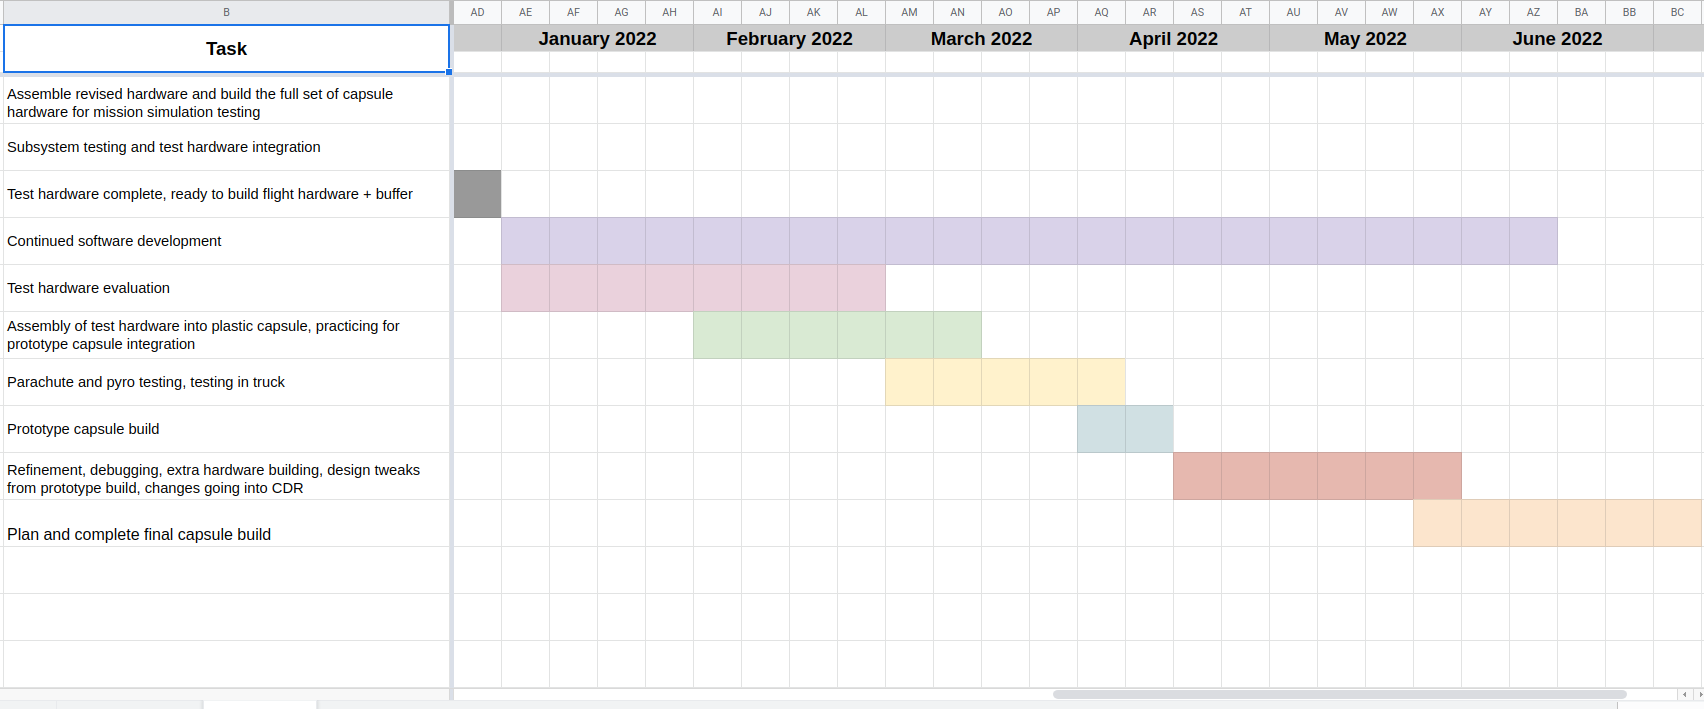
\includegraphics[width=1.25\textwidth]{images/schedule-22.png}
	\caption{Approximate schedule for completion of prototype and final build.}
	\label{fig:schedule22}
\end{figure}

\end{landscape}
\restoregeometry




\newgeometry{margin=2cm} % modify this if you need even more space
\begin{landscape}
\section{Project Schedule Gantt 2021}
\label{app-schedule-21}
This schedule in Fig. \ref{fig:schedule} shows that the project schedule for 2021. The avionics design and assembly process went well and was on schedule moving into 2022.
\begin{figure}[H]
	\centering
	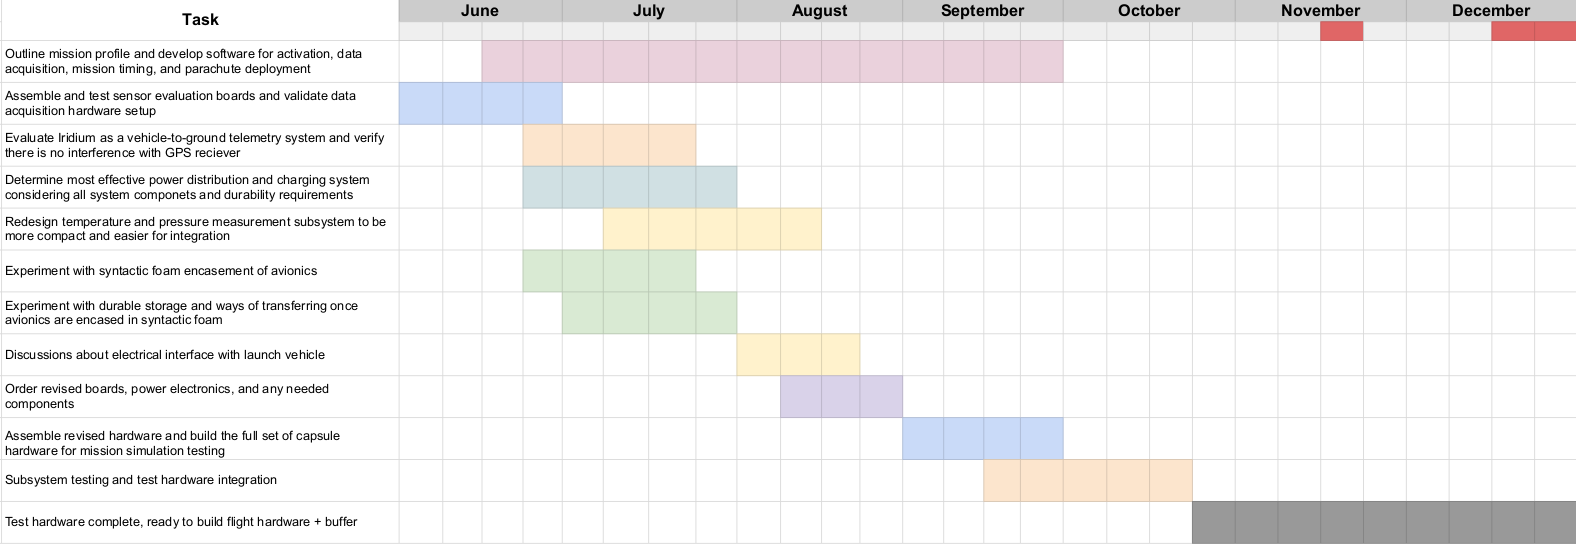
\includegraphics[width=1.25\textwidth]{images/schedule.png}
	\caption{Approximate schedule for completion of prototype and final build.}
	\label{fig:schedule}
\end{figure}
\end{landscape}
\restoregeometry

%\bibliographystyle{plain}
%\bibliography{references}
\end{document}
